\chapter{Frozen Showers}\label{chap:FS}
\minitoc

Fast simulation techniques are an essential part of the Monte Carlo production in the \atlas experiment. The typical time needed for simulating a top pair production event is around one minute. Most of this time is spent on the simulation of particle interaction in the calorimeters. This motivates the development of fast simulation techniques, allowing to describe calorimeter response.

In this chapter, a Frozen Showers method for the forward calorimeter simulation is described. The first section gives a small introduction to the method. In the second section properties of the electron shower in the FCAL are presented. In Sec.~\ref{sec:FSProdUse} the usage of this method is explained. Sec.~\ref{sec:MLBinning} introduces a new procedure of finding initial parameters method. Finally, in the last section, the validation of Frozen Showers accuracy is presented.

\section{Introduction}
Frozen Showers is currently the main fast calorimeter simulation algorithm used in the \atlas experiment\cite{FS}.  It is based on pre-simulated showers, used in the simulation. This method allows reducing the time spent on a simulation of low energy sub showers of the main shower. It gives compared to the full simulation a 25\% speedup. It requires pre-generated libraries of showers for each detector and particle used. 

For each pre-generated shower, its lateral and transverse size and a list of  all energy depositions inside the sensitive material (hits) with information about their energy, position and time are stored. If the energy of a secondary electron in the simulation falls below the cut-off energy, it is replaced by a shower from a library, as presented in Fig.~\ref{fig:MC_FS_method}. The parameters used in the Frozen Showers method are summarized in Tab.~\ref{tab:MC_FS_params}.

\begin{figure}[!tbp]
\center{
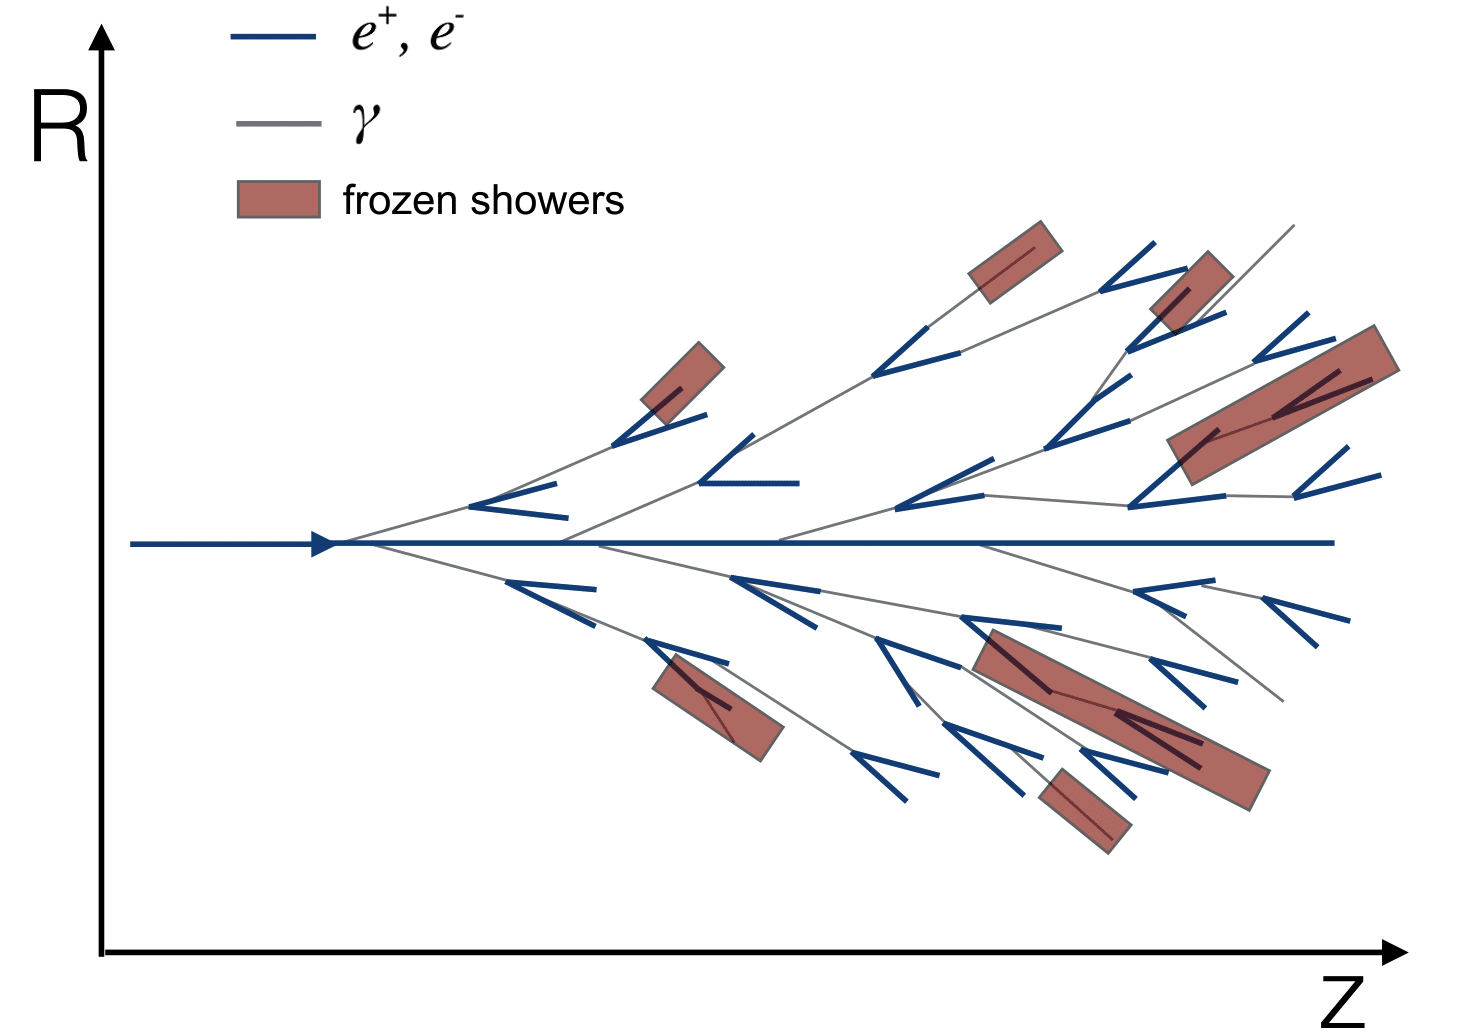
\includegraphics[width=0.9\textwidth]{MC/FSMethod2.png}
\caption{Shower substitution of the low-energy electron, during the high energy electron simulation. Some of the showers from particles, substituted by Frozen Showers method marked by brown squares.}
\label{fig:MC_FS_method}
}
\end{figure}

\begin{table}[!tbp]
\caption{Main parameters used for the frozen shower libraries. The FCAL1 and FCAL2 are the first two froward calorimeters (see Sec.~\ref{sec:forwardCalo}) and $E_{\gamma}$, $E_{e}$, $T_n$ are the maximum energies of photons, electrons and neutrons used in the method. 
}
\label{tab:MC_FS_params}
\centering
\begin{tabular}{l|r}
\hline
\hline
\multicolumn{2}{c}{The general Frozen Showers parameters} \\
\hline
Detectors used            & FCAL1, FCAL2\\
Type of the particle      & photons, electrons, neutrons \\
Energy cut-off            &  $E_{\gamma}<10$~MeV,  $E_{e}<1000$~MeV,  $E_n<100$~MeV \\
\hline
\end{tabular}
\end{table}

\section{Properties of electron showers in FCAL}\label{sec:FSproblem}




%\begin{figure}[!b]
%\center{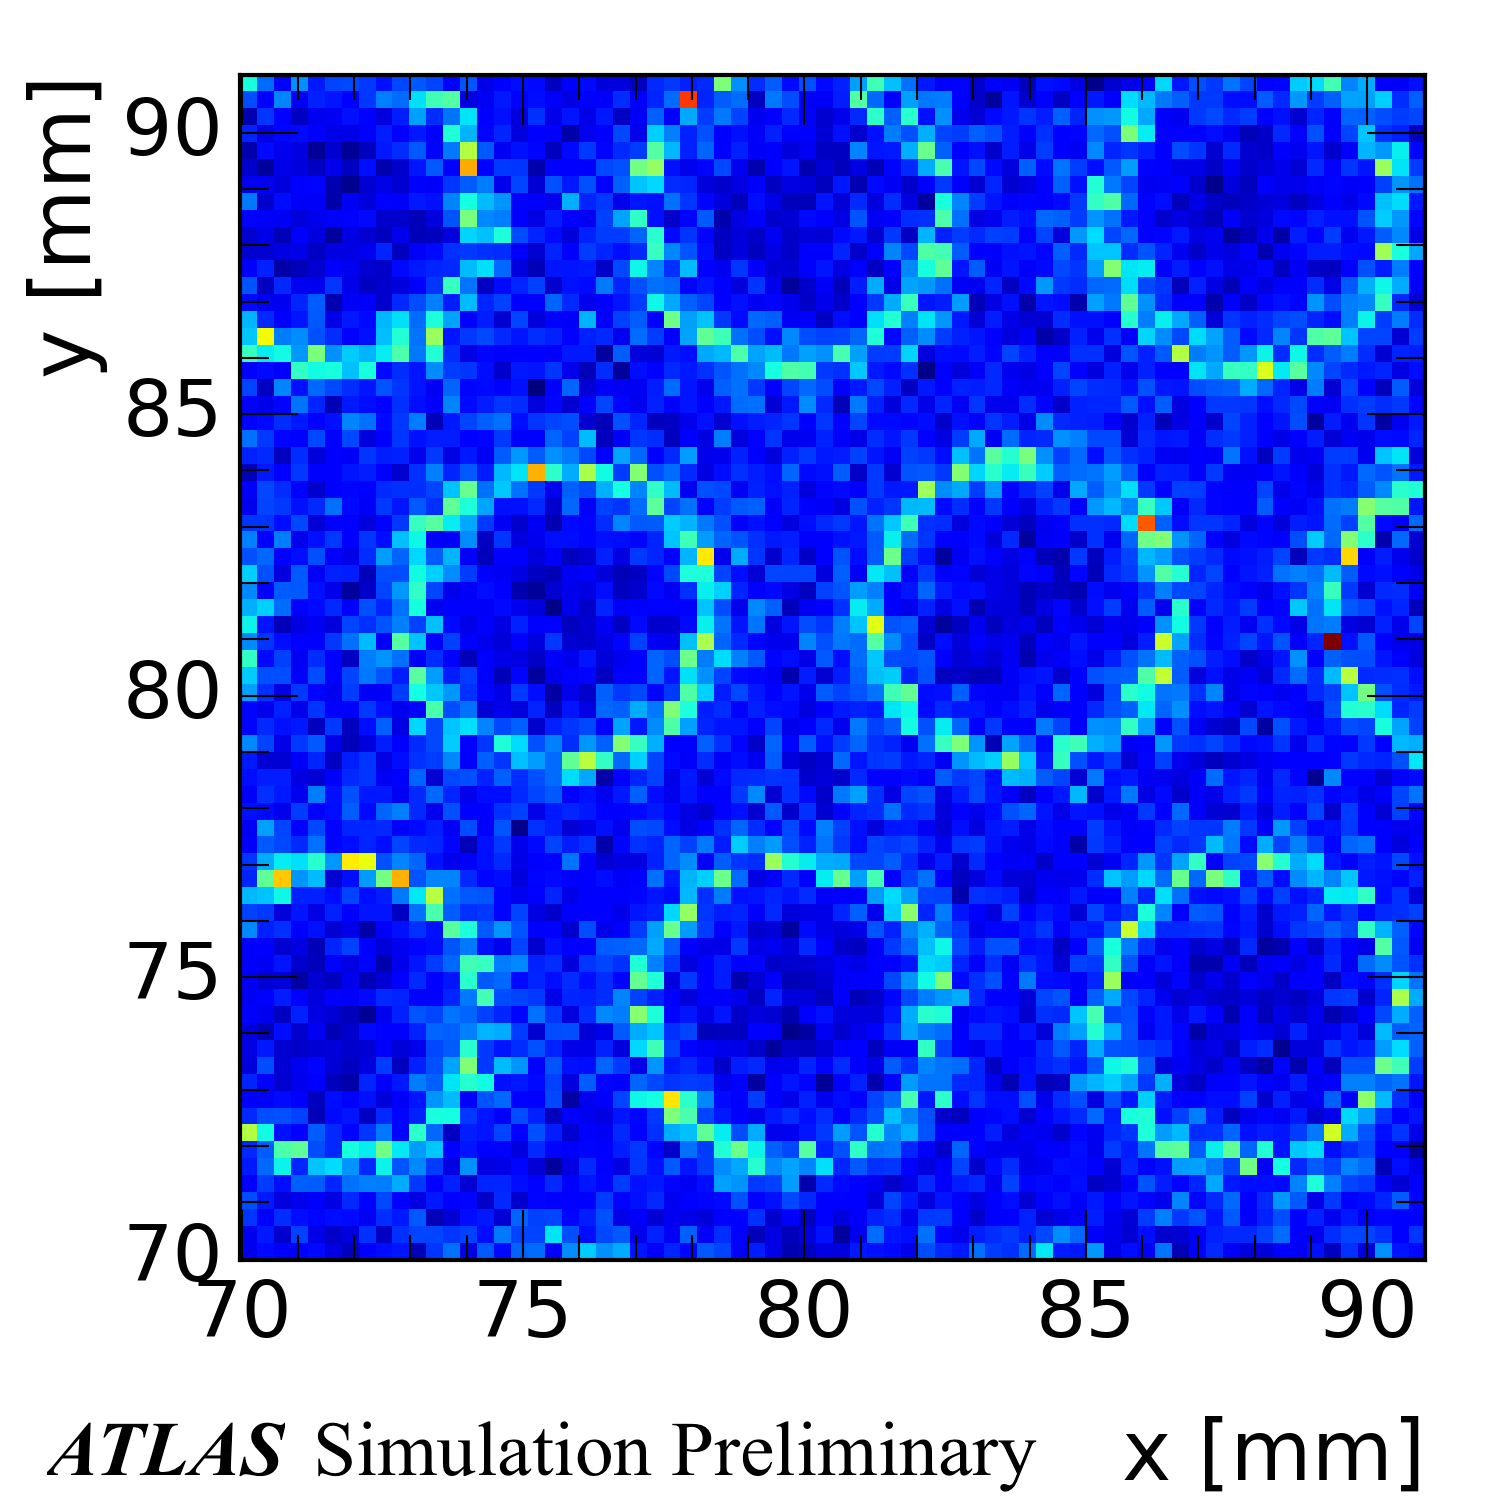
\includegraphics[width=0.5\linewidth]{MC/xySumE.png} }
%\caption{Shower energy response histogram in the x vs y plane for electrons, generated with uniformly distributed x and y and energy less than 1 GeV. Light circles are corresponding to a showers, started inside a LAr gaps with on average higher energy response, while the dark parts are corresponding to dead material respectively with smaller sum of the "hits" energy. }
%\label{fig:FSFluctuations}
%\end{figure}

\begin{figure}[!tbp]
\begin{minipage}[h]{0.49\linewidth}
\center{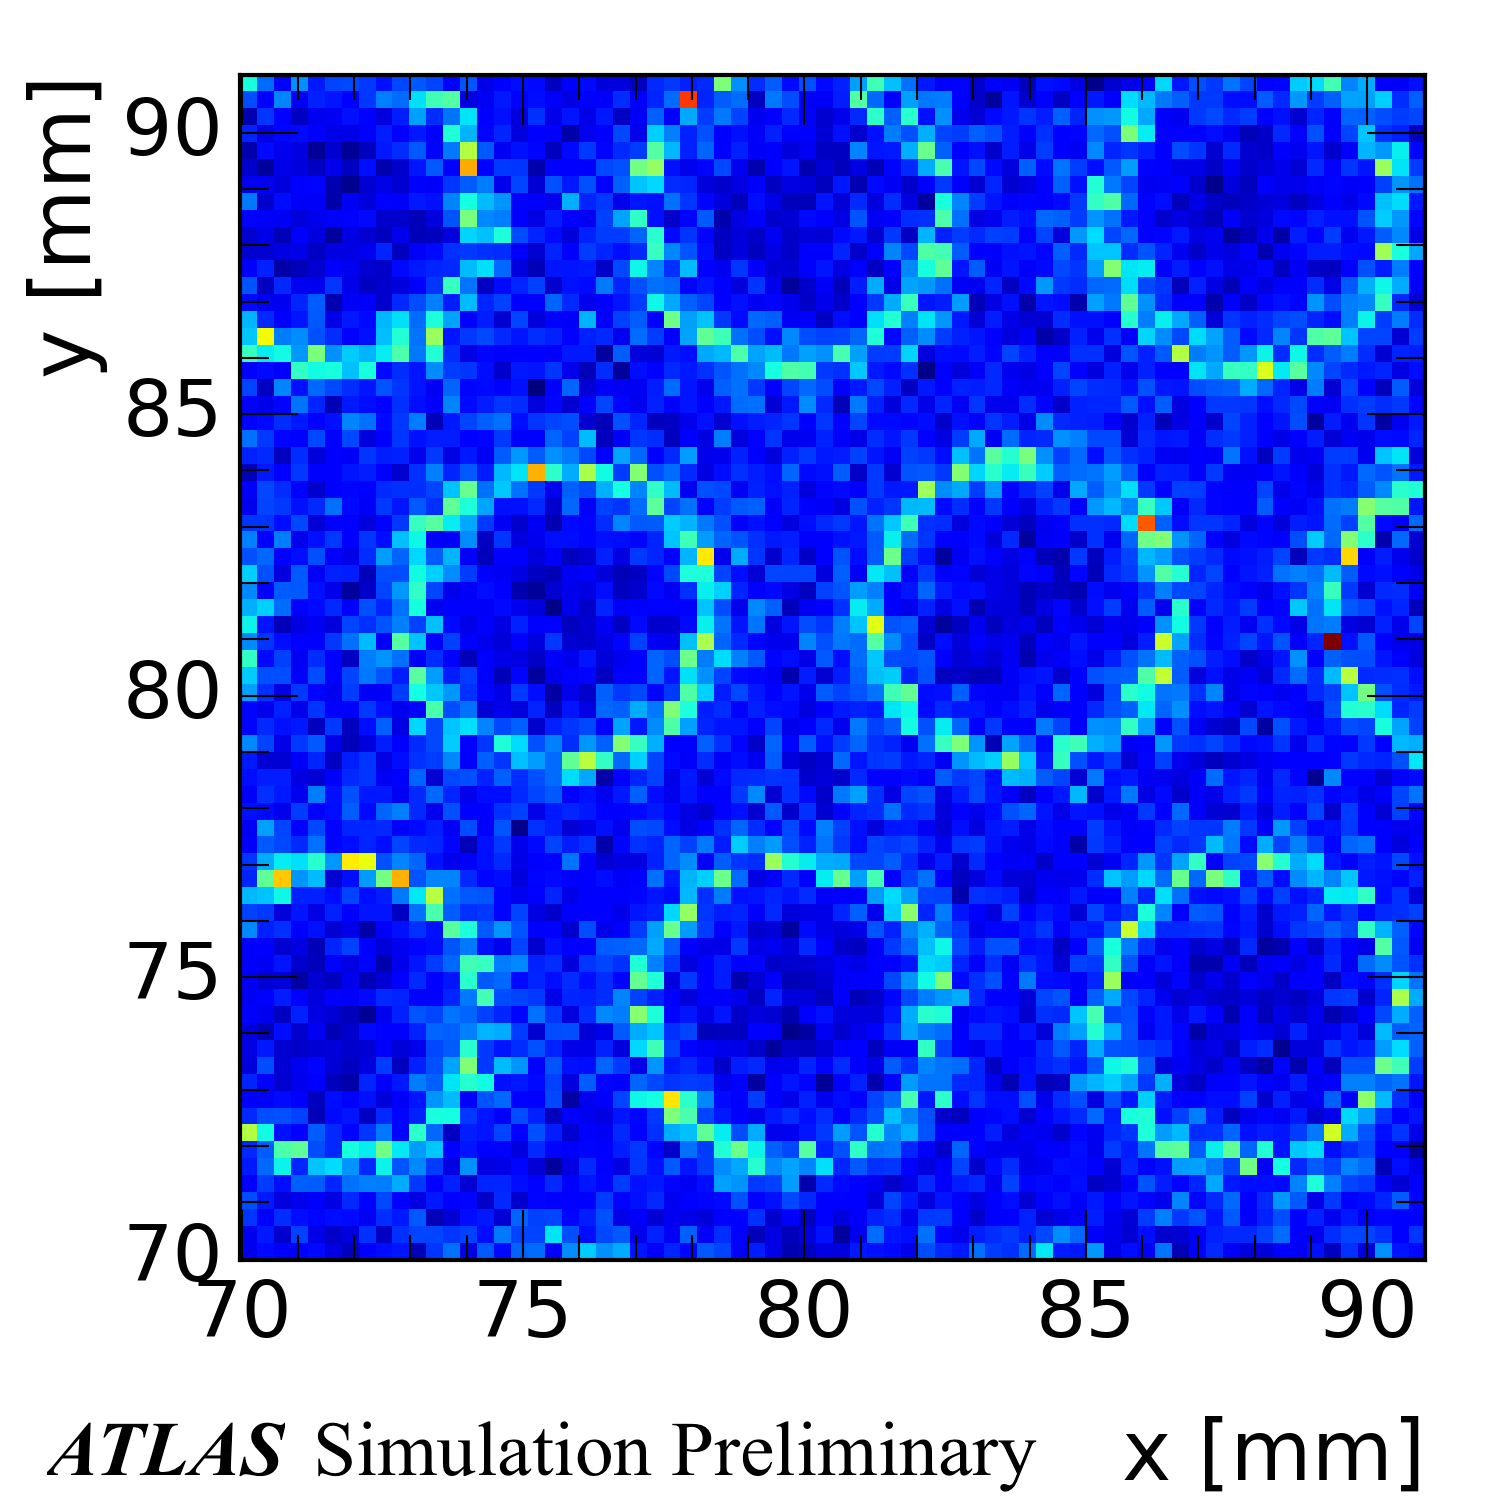
\includegraphics[width=0.9\linewidth]{MC/xySumE.png} \\ a)}
\end{minipage}
\hfill
\begin{minipage}[h]{0.49\linewidth}
\center{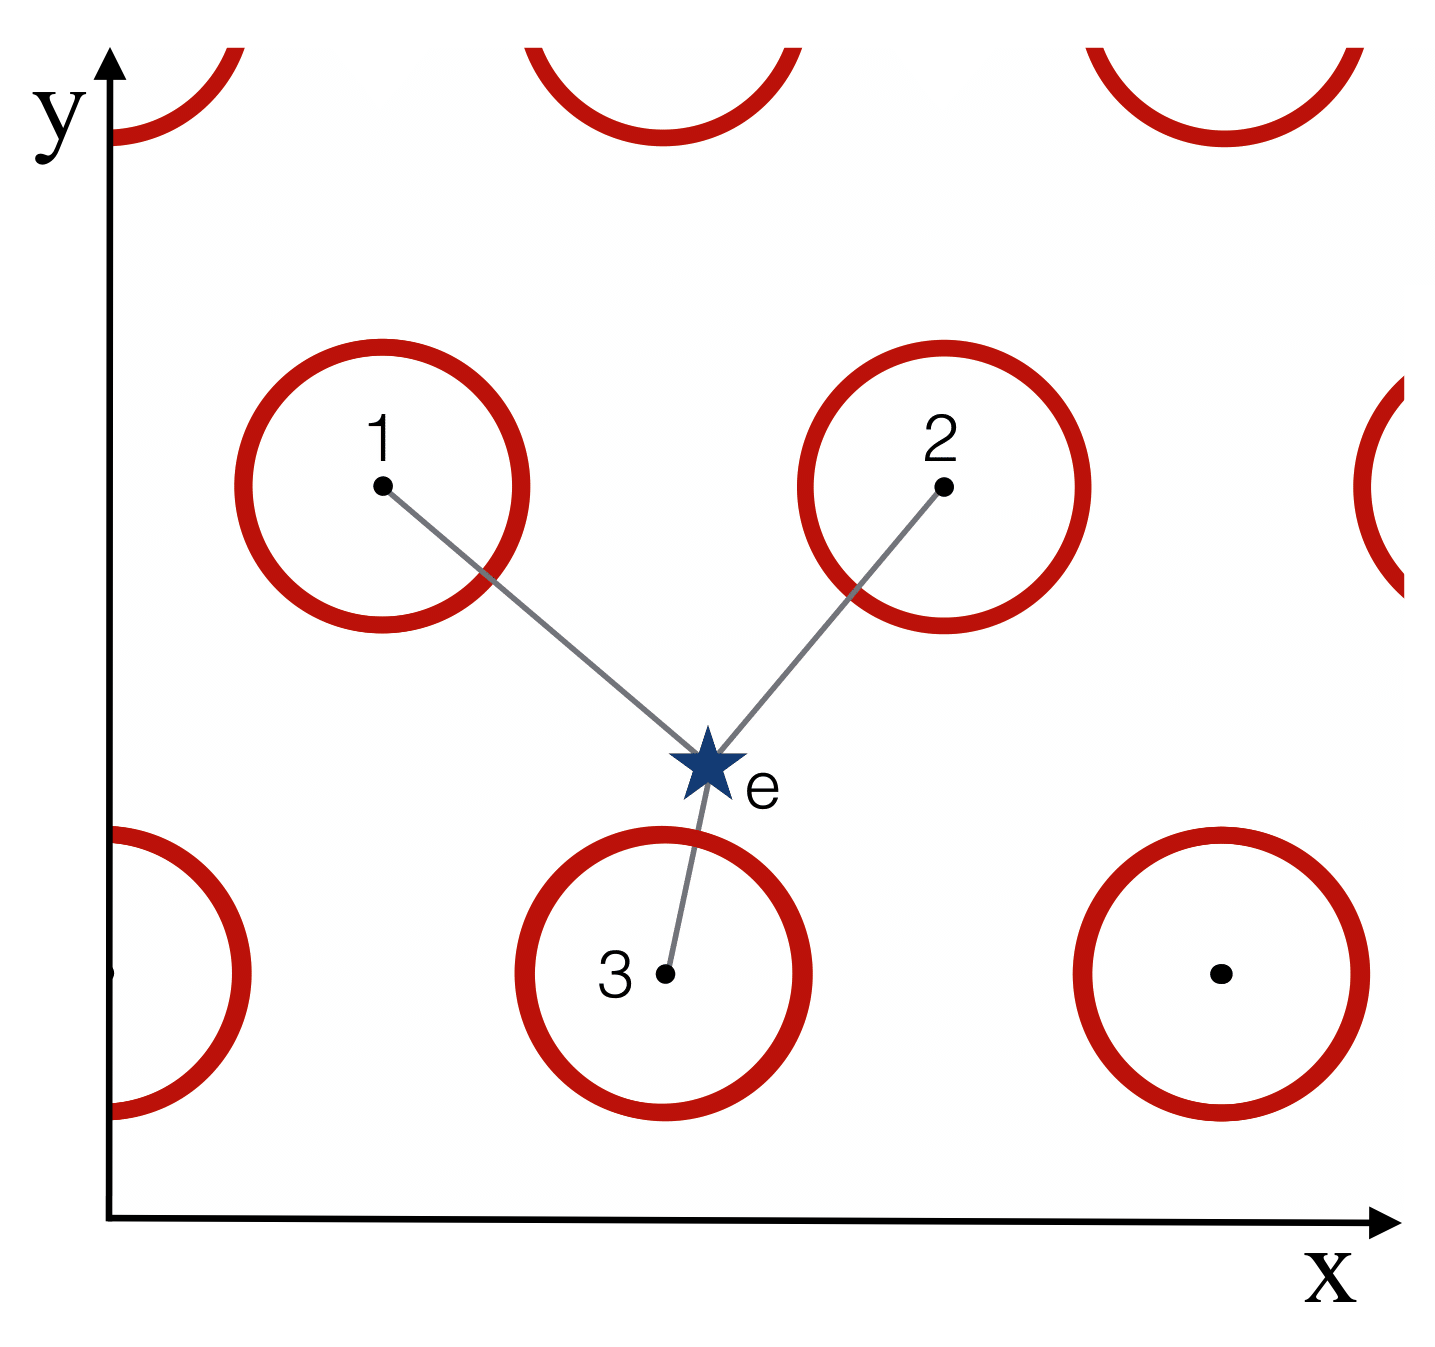
\includegraphics[width=0.9\linewidth]{MC/DistanceCalculation.png} \\b)}
\end{minipage}
\caption{ a) Electron shower energy response  in the transverse FCAL plane. Light circles correspond to showers, developing inside the LAr gaps with on average higher energy response, while a dark parts correspond to dead material with a smaller sum of the "hits" energy.
b) Distance to the closest rod center scheme. The rod centers and liquid argon gaps are shown by black dots and red circles respectively.}
%\caption{Distribution a) electron energies and b) mean number of hits in a shower vs energy of electron for electrons with energy less than 1 GeV coming from initial electron with energy 1 TeV. }
\label{fig:FSFluctuations}
\end{figure}


\begin{figure}[!tbp]
\begin{minipage}[h]{0.49\linewidth}
\center{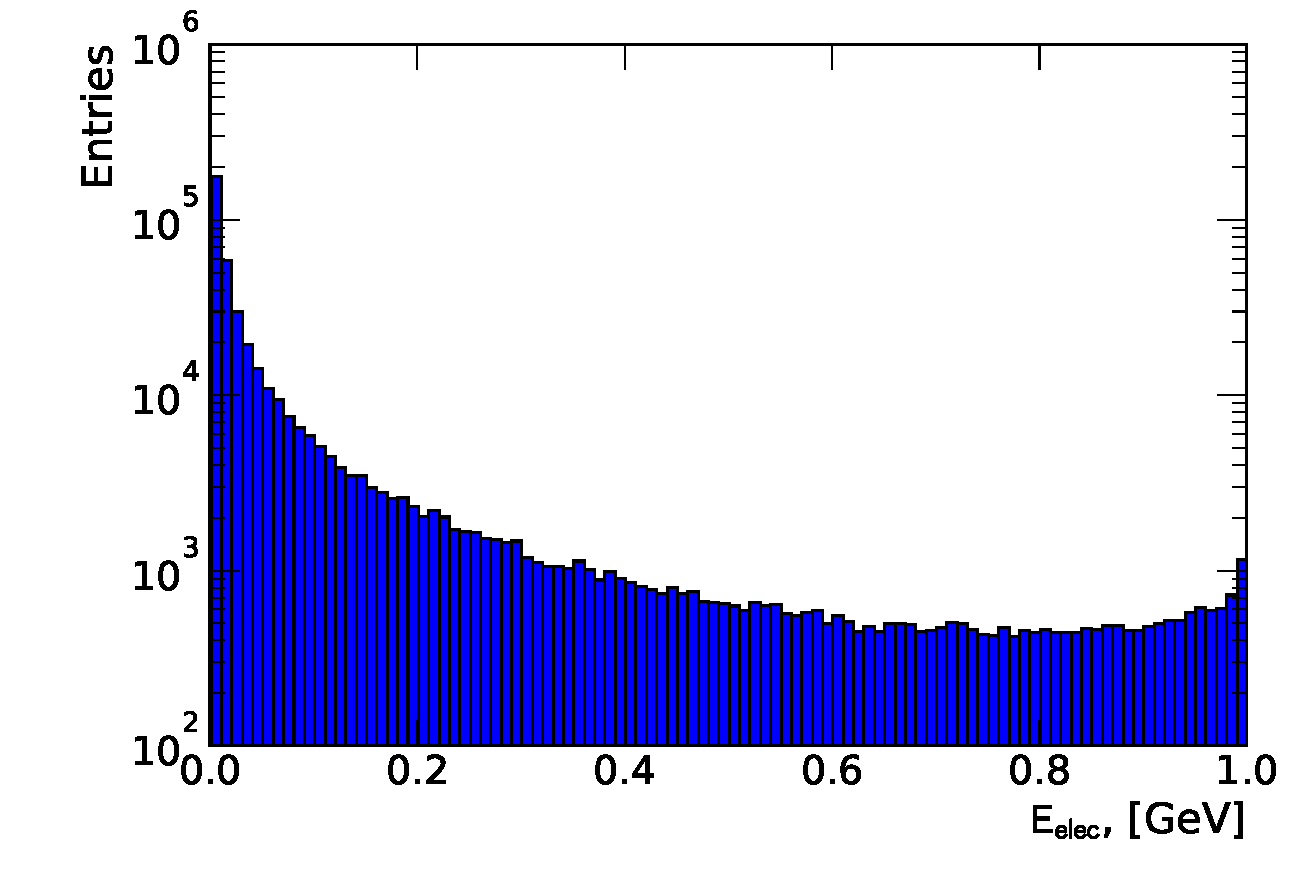
\includegraphics[width=1.0\linewidth]{MC/FSEnergy.pdf}  \\ a)}
\end{minipage}
\hfill
\begin{minipage}[h]{0.49\linewidth}
\center{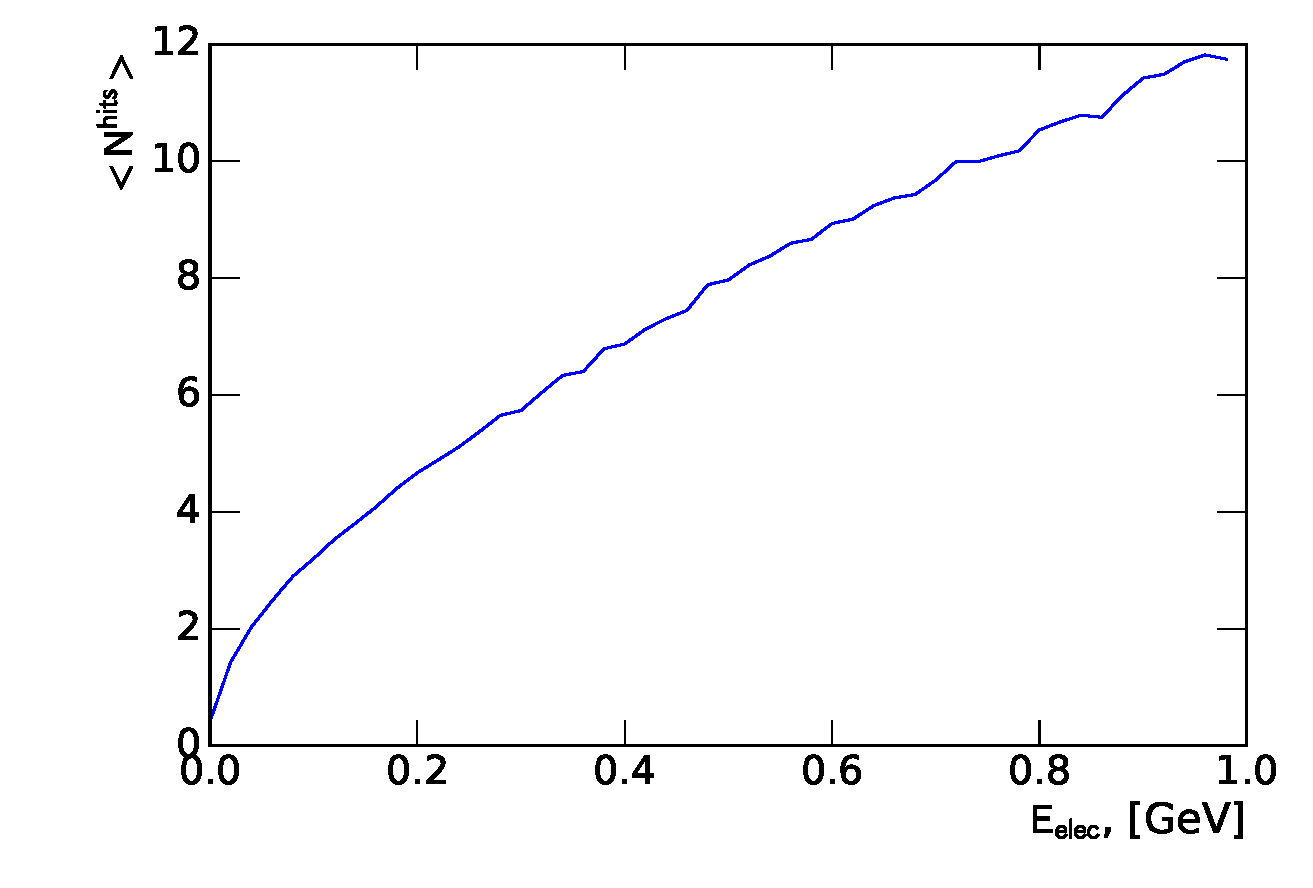
\includegraphics[width=1.0\linewidth]{MC/nHitsMean.pdf} \\ b)}
\end{minipage}
\caption{Distribution  of the a) electron energies and b) a mean number of hits in the shower vs energy of electron for electrons used in the generation of 1 TeV electron.}
\label{fig:TrackEnergy}
\end{figure}

The fast simulation of  the \atlas forward calorimeters is a complicated task, due to the complex structure. As it is mentioned in Sec.~\ref{sec:forwardCalo} FCAL consists of hexagonal absorber cells with the anode tube and cathode rod in the cell center and the liquid argon in the gap between the rod and tube. An efficient fast simulation technique should take into account this significant amount of non-uniformly distributed sensitive material to simulate electron resolution correctly.

The electron energy resolution of a calorimeter can be written as\cite{Vovenko1983}:
\begin{equation}\label{eq:EMResoultion}
\frac{\sigma}{E} \approx \frac{1}{\sqrt{E}}	\oplus \frac{1}{E} 	\oplus const,
\end{equation}
where $\oplus$ indicates the quadratic sum. The first term is the 'stochastic term', which includes intrinsic shower fluctuations, the second  one takes into account readout noise effects and pile-up fluctuations. The $const$ term is connected to non-uniformities in the detector, causing significant fluctuations of the energy loss. The constant term dominates the typical energy resolution for high energy electrons. 

Fluctuations due to the detector design can be observed in the simulation of low-energy electrons. The shower energy ($E^{shower}$) distribution in the transverse FCAL plane is shown in Fig.~\ref{fig:FSFluctuations} (a). The shower energy is defined as:
\begin{equation}
E^{shower}=\sum E_i^{hits},
\end{equation}
where $E_i^{hits}$ is the energy of the $i$-th hit in the shower inside the sensitive detector material. The periodic structure resembles the calorimeter design, where the light circles correspond to gaps with the liquid argon sensitive material. The distance to the closest rod center for the initial electron is calculated as (Fig.~\ref{fig:FSFluctuations}):
\begin{equation}
d_{rod} = min( d(1,e), d(2, e), d(3, e)),
\end{equation} 
where 1,2,3 are the positions of the rod centers and $e$ is the position of the initial electron.

Most of the electrons, substituted by the Frozen Showers algorithm have a low energy (Fig.~\ref{fig:TrackEnergy} a).   The mean number of deposits in the sensitive material for the shower from the Frozen Showers algorithm is around 5 and this value rises with the electron energy (Fig.~\ref{fig:TrackEnergy} b).  Fig.~\ref{fig:FSProduction} presents the distribution of the distance to the closest rod center and shower energies for Frozen Showers used in the simulation of 1 TeV electrons. There is a visible peak of shower energy for the region around liquid argon gap, marked by the red lines. A similar structure is also visible in a number of depositions in the sensitive material (Fig.~\ref{fig:ShowerProp} a) and the standard deviation of the hits energies in the shower (Fig.~\ref{fig:ShowerProp} b) distributions. The magnitude of the peak depending on the electron energy and is higher for the low energies (Fig.~\ref{fig:FSProduction2} a) and less significant for higher energies (Fig.~\ref{fig:FSProduction2} b). The proper simulation method should be able to reproduce these distributions in the simulation.

\begin{figure}[!tbp]
\center{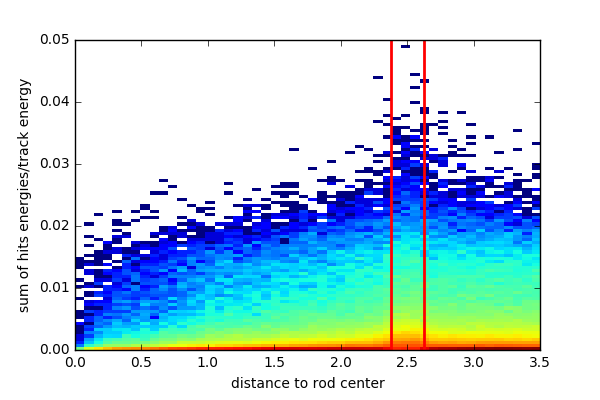
\includegraphics[width=1.\linewidth]{MC/fullBinningScatter.png} }
\caption{Distribution of distance to the closest rod center vs shower energy for electron showers created by electrons used in the generation of 1 TeV electron in the distance to the closest rod center vs shower energy plane. Red lines note the position of the liquid argon gap. }
\label{fig:FSProduction}
\end{figure}

\begin{figure}[!tbp]
\begin{minipage}[h]{0.49\linewidth}
\center{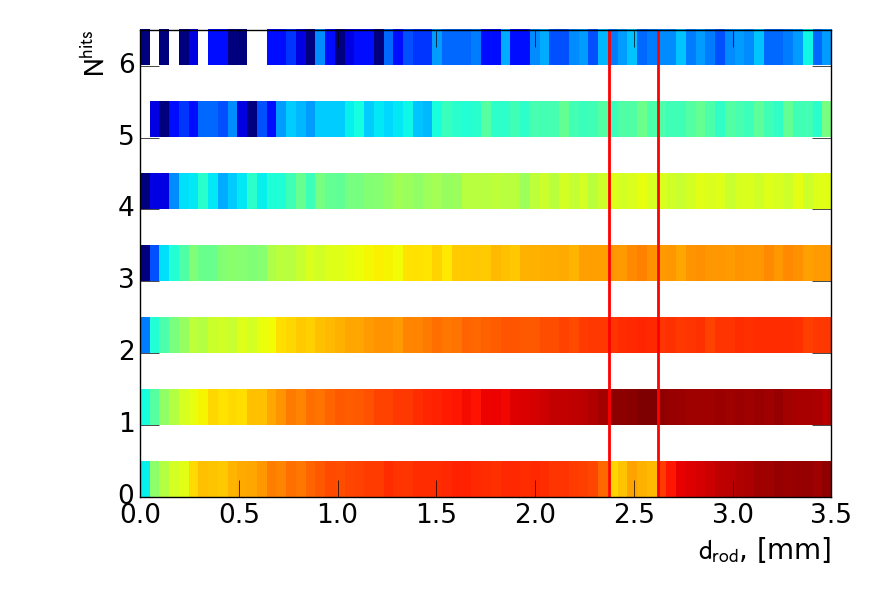
\includegraphics[width=1.0\linewidth]{MC/nHits.png}  \\ a)}
\end{minipage}
\hfill
\begin{minipage}[h]{0.49\linewidth}
\center{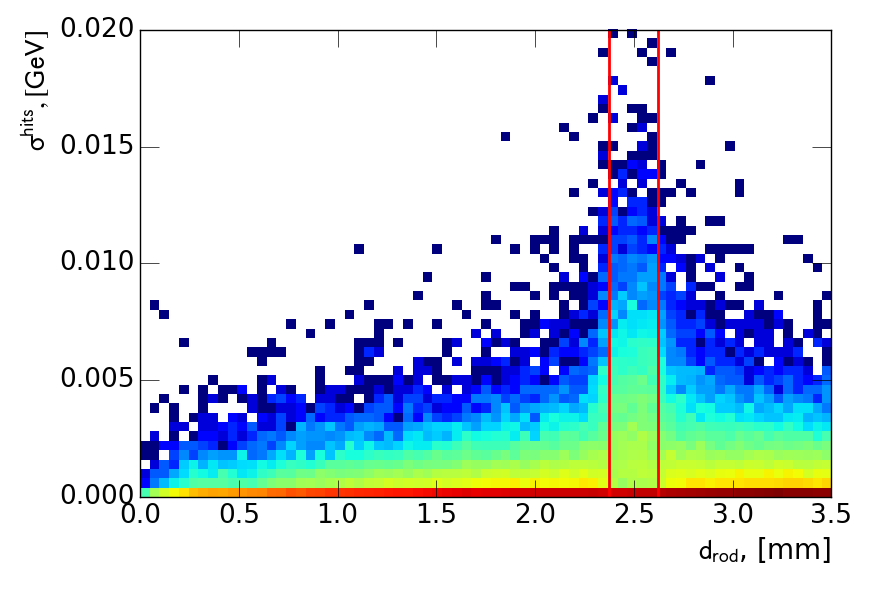
\includegraphics[width=1.0\linewidth]{MC/rms.png} \\ b)}
\end{minipage}
\caption{Distribution of distance to the closest rod center vs a) number of hits in a shower plane and b) standard deviation of hits in a shower energy of electron showers from electrons used in the generation of 1 TeV electron. Red lines note the position of the liquid argon gap.}
\label{fig:ShowerProp}
\end{figure}

\begin{figure}[!tbp]
\begin{minipage}[h]{0.49\linewidth}
\center{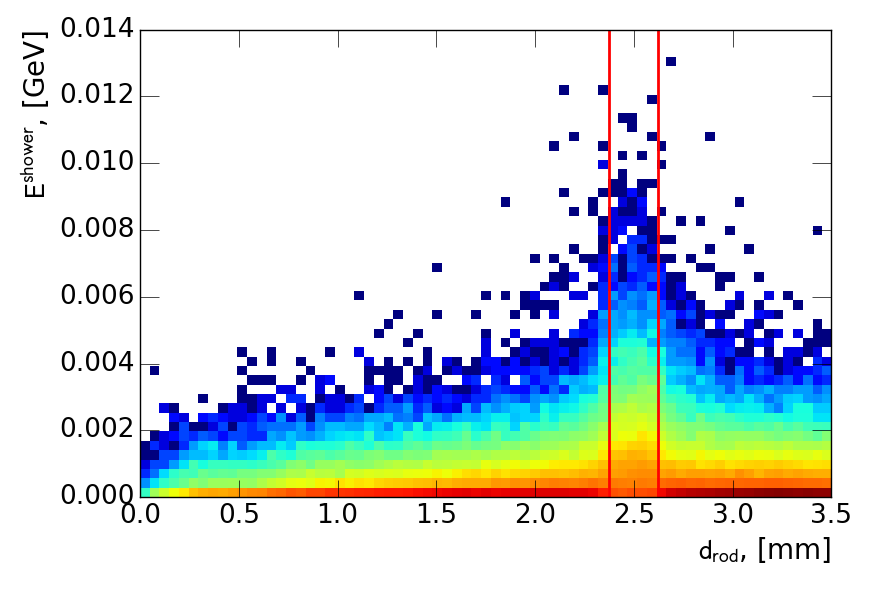
\includegraphics[width=1.\linewidth]{MC/fullBinningScatterSmall.png} \\ a)}
\end{minipage}
\hfill
\begin{minipage}[h]{0.49\linewidth}
\center{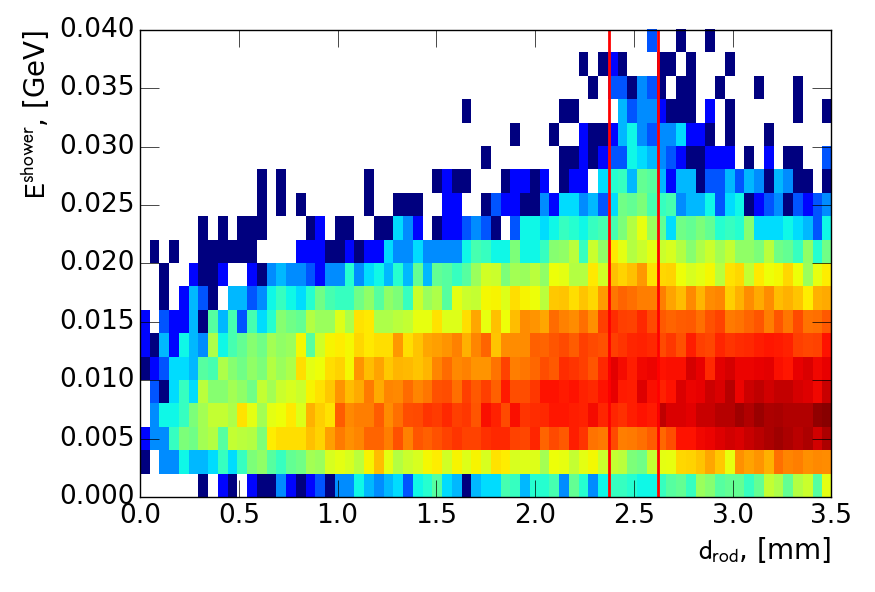
\includegraphics[width=1.\linewidth]{MC/fullBinningScatterBig.png} \\ b)}
\end{minipage}
\caption{Distribution of distance to the closest rod center vs shower energy for electron showers created by electrons with energy a) less than 100 MeV  and b) higher than 300 GeV coming from the initial electron with energy 1 TeV.   Red lines note the position of the liquid argon gap.}
\label{fig:FSProduction2}
\end{figure}

It should be noted, that this method is applicable for the full energy range of the electrons. For the high energy electrons, this method gives no significant speedup compared to the full simulation.  Use of the Frozen Showers in the small electron energy region can be suboptimal, due to the low number of energy depositions in sensitive material. Most of the electrons with energy below 30 MeV have no hits in the sensitive material (Fig.~\ref{fig:fracHits} a) and only 0.5\% produce more than one hit (Fig.~\ref{fig:fracHits} b). The studies of the Frozen Showers algorithm performance have shown, that introduction of the 30 MeV lower threshold for the algorithm allows to reduce time spent on the simulation of the high-energy electrons. The electrons with energy below 30 MeV are substituted by the single hit in the detector.

\begin{figure}[!tbp]
\begin{minipage}[h]{0.49\linewidth}
\center{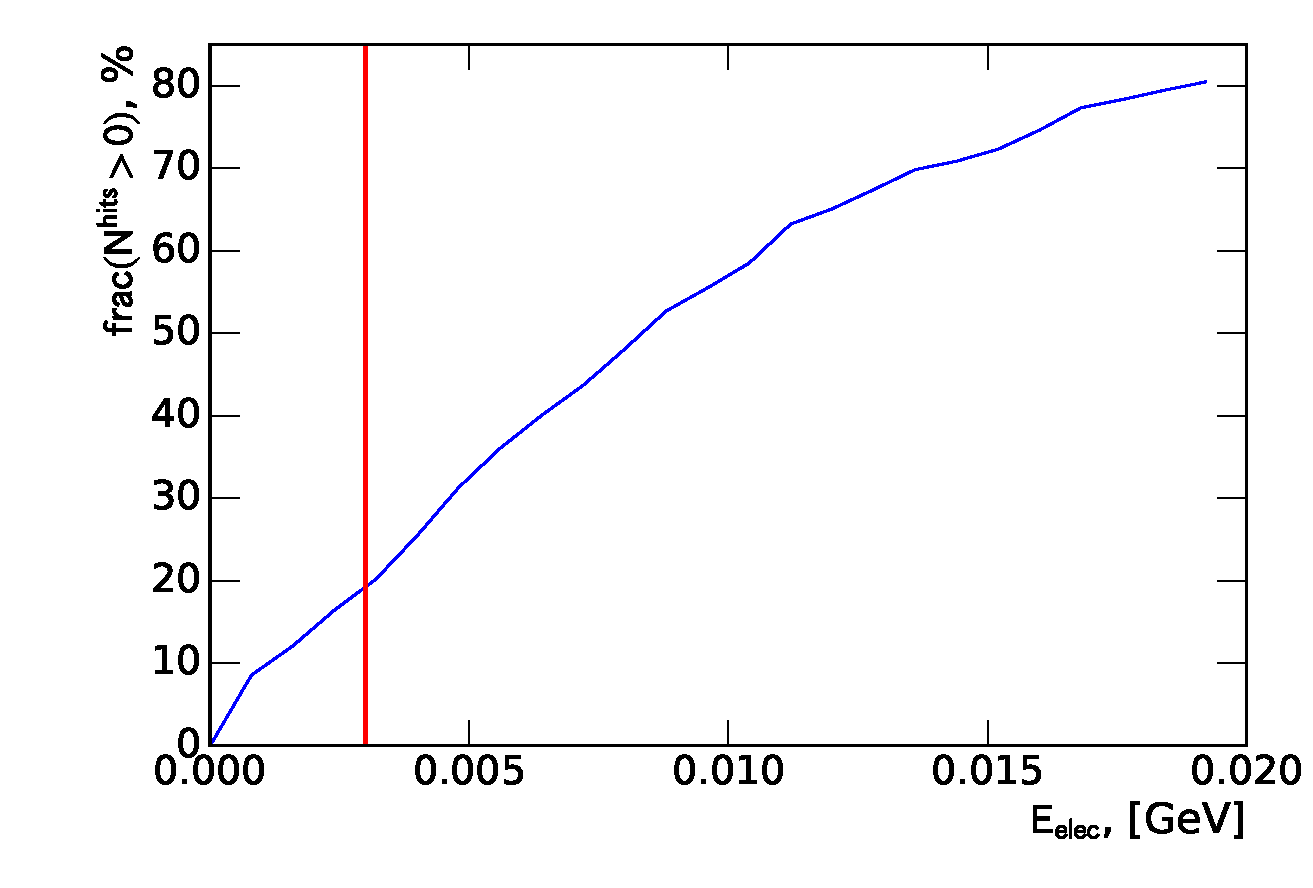
\includegraphics[width=1.\linewidth]{MC/fracHits2.pdf} \\ a)}
\end{minipage}
\hfill
\begin{minipage}[h]{0.49\linewidth}
\center{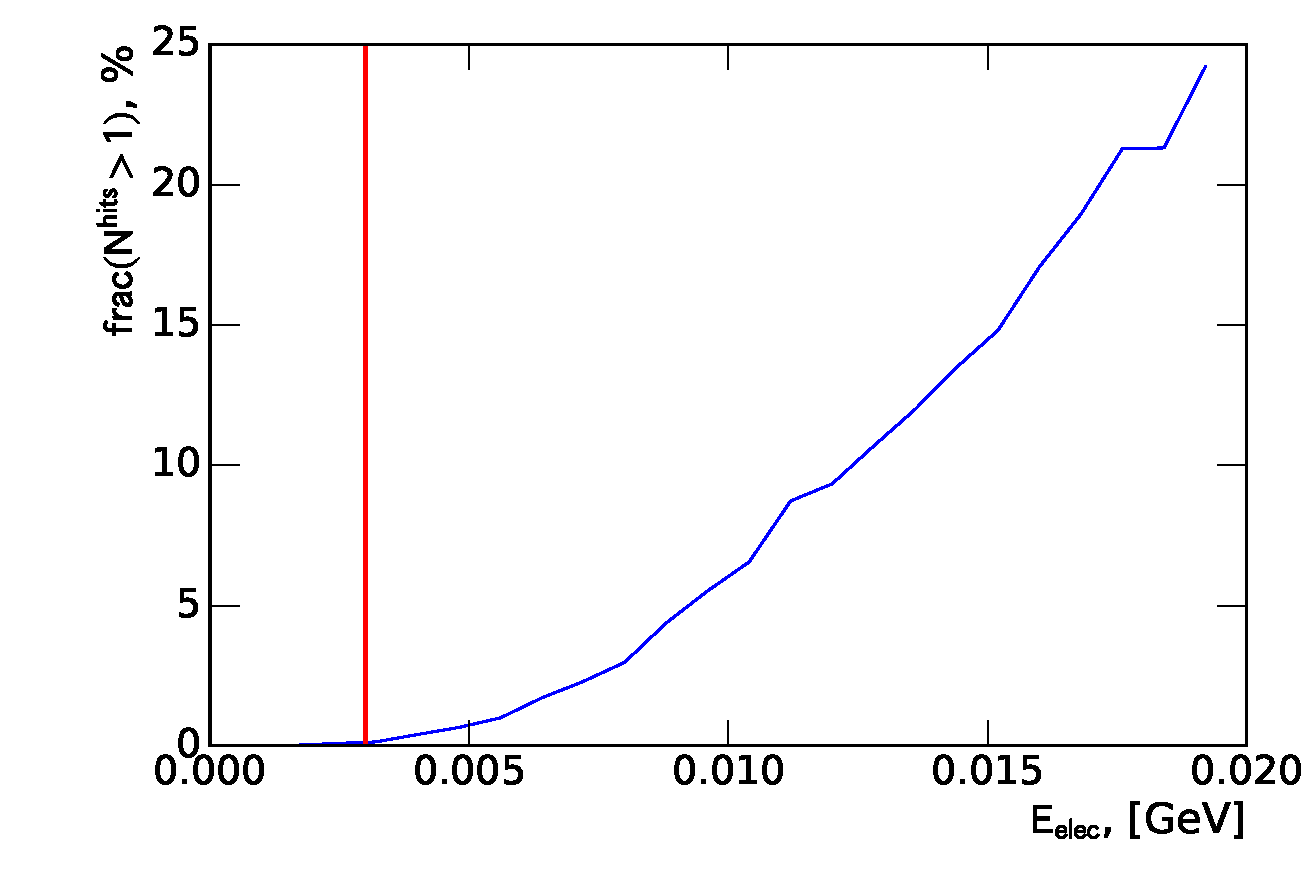
\includegraphics[width=1.\linewidth]{MC/fracHits.pdf} \\ b)}
\end{minipage}
\caption{The fraction of showers with a) at least 1 b) at least two depositions inside the sensitive material as a function of the initial electron energy. The red line denotes the 30 MeV lower limit applied in the Frozen Showers method.}
\label{fig:fracHits}
\end{figure}


\section{Generation and use in simulation}\label{sec:FSProdUse}

The Frozen Showers method consists of two stages: generation of libraries and the use in simulation. The generation process is repeated after each significant change in the simulation (e.g. detector or physics process description). Pre-simulated showers are parameterized in bins of pseudorapidity and distance to the closest rod center, while the energy of the initial electrons remains unbinned. One of the distances to the closest rod center bin position matches to the position of the liquid argon gap. The corresponding bin  (called \textit{liquid argon bin}) is introduced to simulate the peak in the distributions described in Sec.~\ref{sec:FSproblem}. 

In simulation, particles originating from SM processes are used. The hit information is compressed in two steps: 
\begin{description}
\item [Hit merging] If the distance between any two hits is smaller than a given parameter $R_{min}$, then the hits are merged into one deposit at the energy barycenter of the hits;
\item [Truncation] The hits with the energy below the cutoff energy are truncated. The energy of the remaining hits is rescaled to preserve the total deposited energy.
\end{description}

During the simulation, if the energy of a particle falls below a cut-off energy, the Frozen Showers algorithm examines the resulting shower. The algorithm how far  from the edges of the calorimeter the particle, such that the shower energy is by 90\% contained inside the calorimeter. The containment depends on position and energy of the initial particle (since the  shower size grows with  the particle energy). The algorithm matches the particle with the given entry in the Frozen Showers library. To correct for the differences in the energy between the initial particle and a matched library entry, each hit in the shower is scaled as:
\begin{equation}
E_{hit}^{new}=E_{hit}\cdot \frac{E_{part}}{E_{part,lib}},
\end{equation}
where $E_{hit}$ is the energy of the hit, $E_{part}$ is the energy of the particle and $E_{part,lib}$ is the energy of the particle stored in the library. In the final step, the particle is substituted by the resulting shower and the reconstruction algorithm uses these hits from this shower hits in the sensitive material.


\subsection{Tuning procedure}\label{sec:LibTuning}

The fast simulation method is required to be consistent with full simulation. In case of Frozen Showers in FCAL, the electron energy resolution is problematic to describe by the model, since the resolution of the reconstructed electrons found to be around two times smaller (Fig.~\ref{fig:FS_resolution}), than in the full simulation. Using the Eq.~\ref{eq:EMResoultion}, this behavior can be interpreted due to a too small size of fluctuations introduced in fast simulation and consequently a lack of the high-energy showers starting in sensitive material. This problem can be solved by tuning the parameters of the library to match the full simulation.

The tuning procedure consists of two steps:
\begin{description}
\item [Bin width change] At this stage the width of the liquid argon bin is enlarged. This procedure causes a higher number of showers with large energy response in simulation (and therefore higher fluctuations). This procedure causes an increase in simulated energy scale and resolution;
\item [Shower energy scaling] The shower energy is rescaled to correct the shift in the mean reconstructed energies.
\end{description}
This procedure is repeated iteratively in each pseudorapidity bin separately until the desired agreement between full and fast simulation is obtained. The resulting liquid argon bin positions for different pseudorapidity bins are shown in Fig.~\ref{fig:FSOldTuning}. This method yields a relatively good agreement with full simulation (black dots in Fig.~\ref{fig:FS_resolution}). However, due to the large manpower needed, this method is not optimal and requires some optimization.


\begin{figure}[!tbp]
\center{
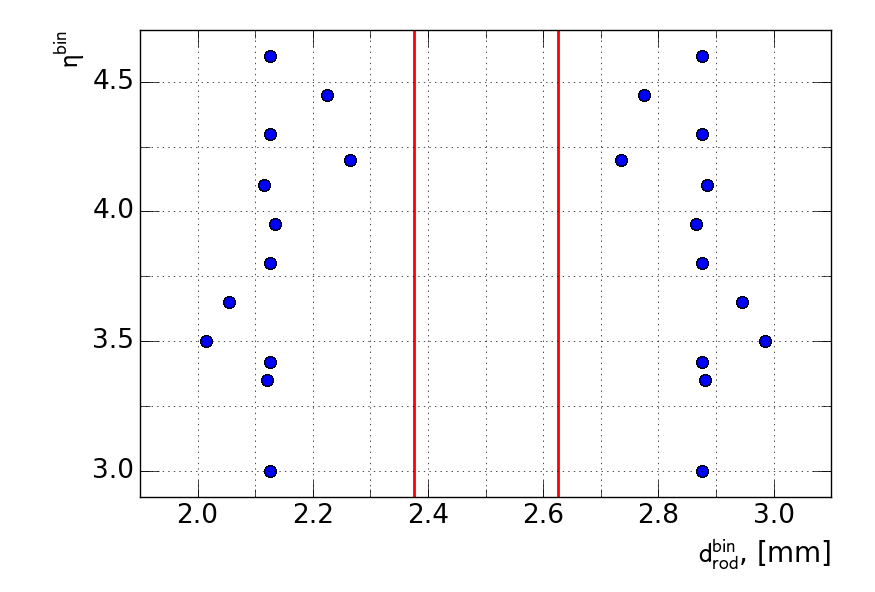
\includegraphics[width=0.8\textwidth]{MC/oldTuning.png}
\caption{The position of liquid argon gap bins for different $\eta$ bins after the tuning procedure. Dots correspond to the each $\eta$ and distance to the closest rod center bin positions. The red lines are denoting the original position of the distance to the closest rod center bins and correspond to the position of the liquid argon gap in the calorimeter.}
\label{fig:FSOldTuning}}
\end{figure}

\begin{figure}[!tbp]
\center{
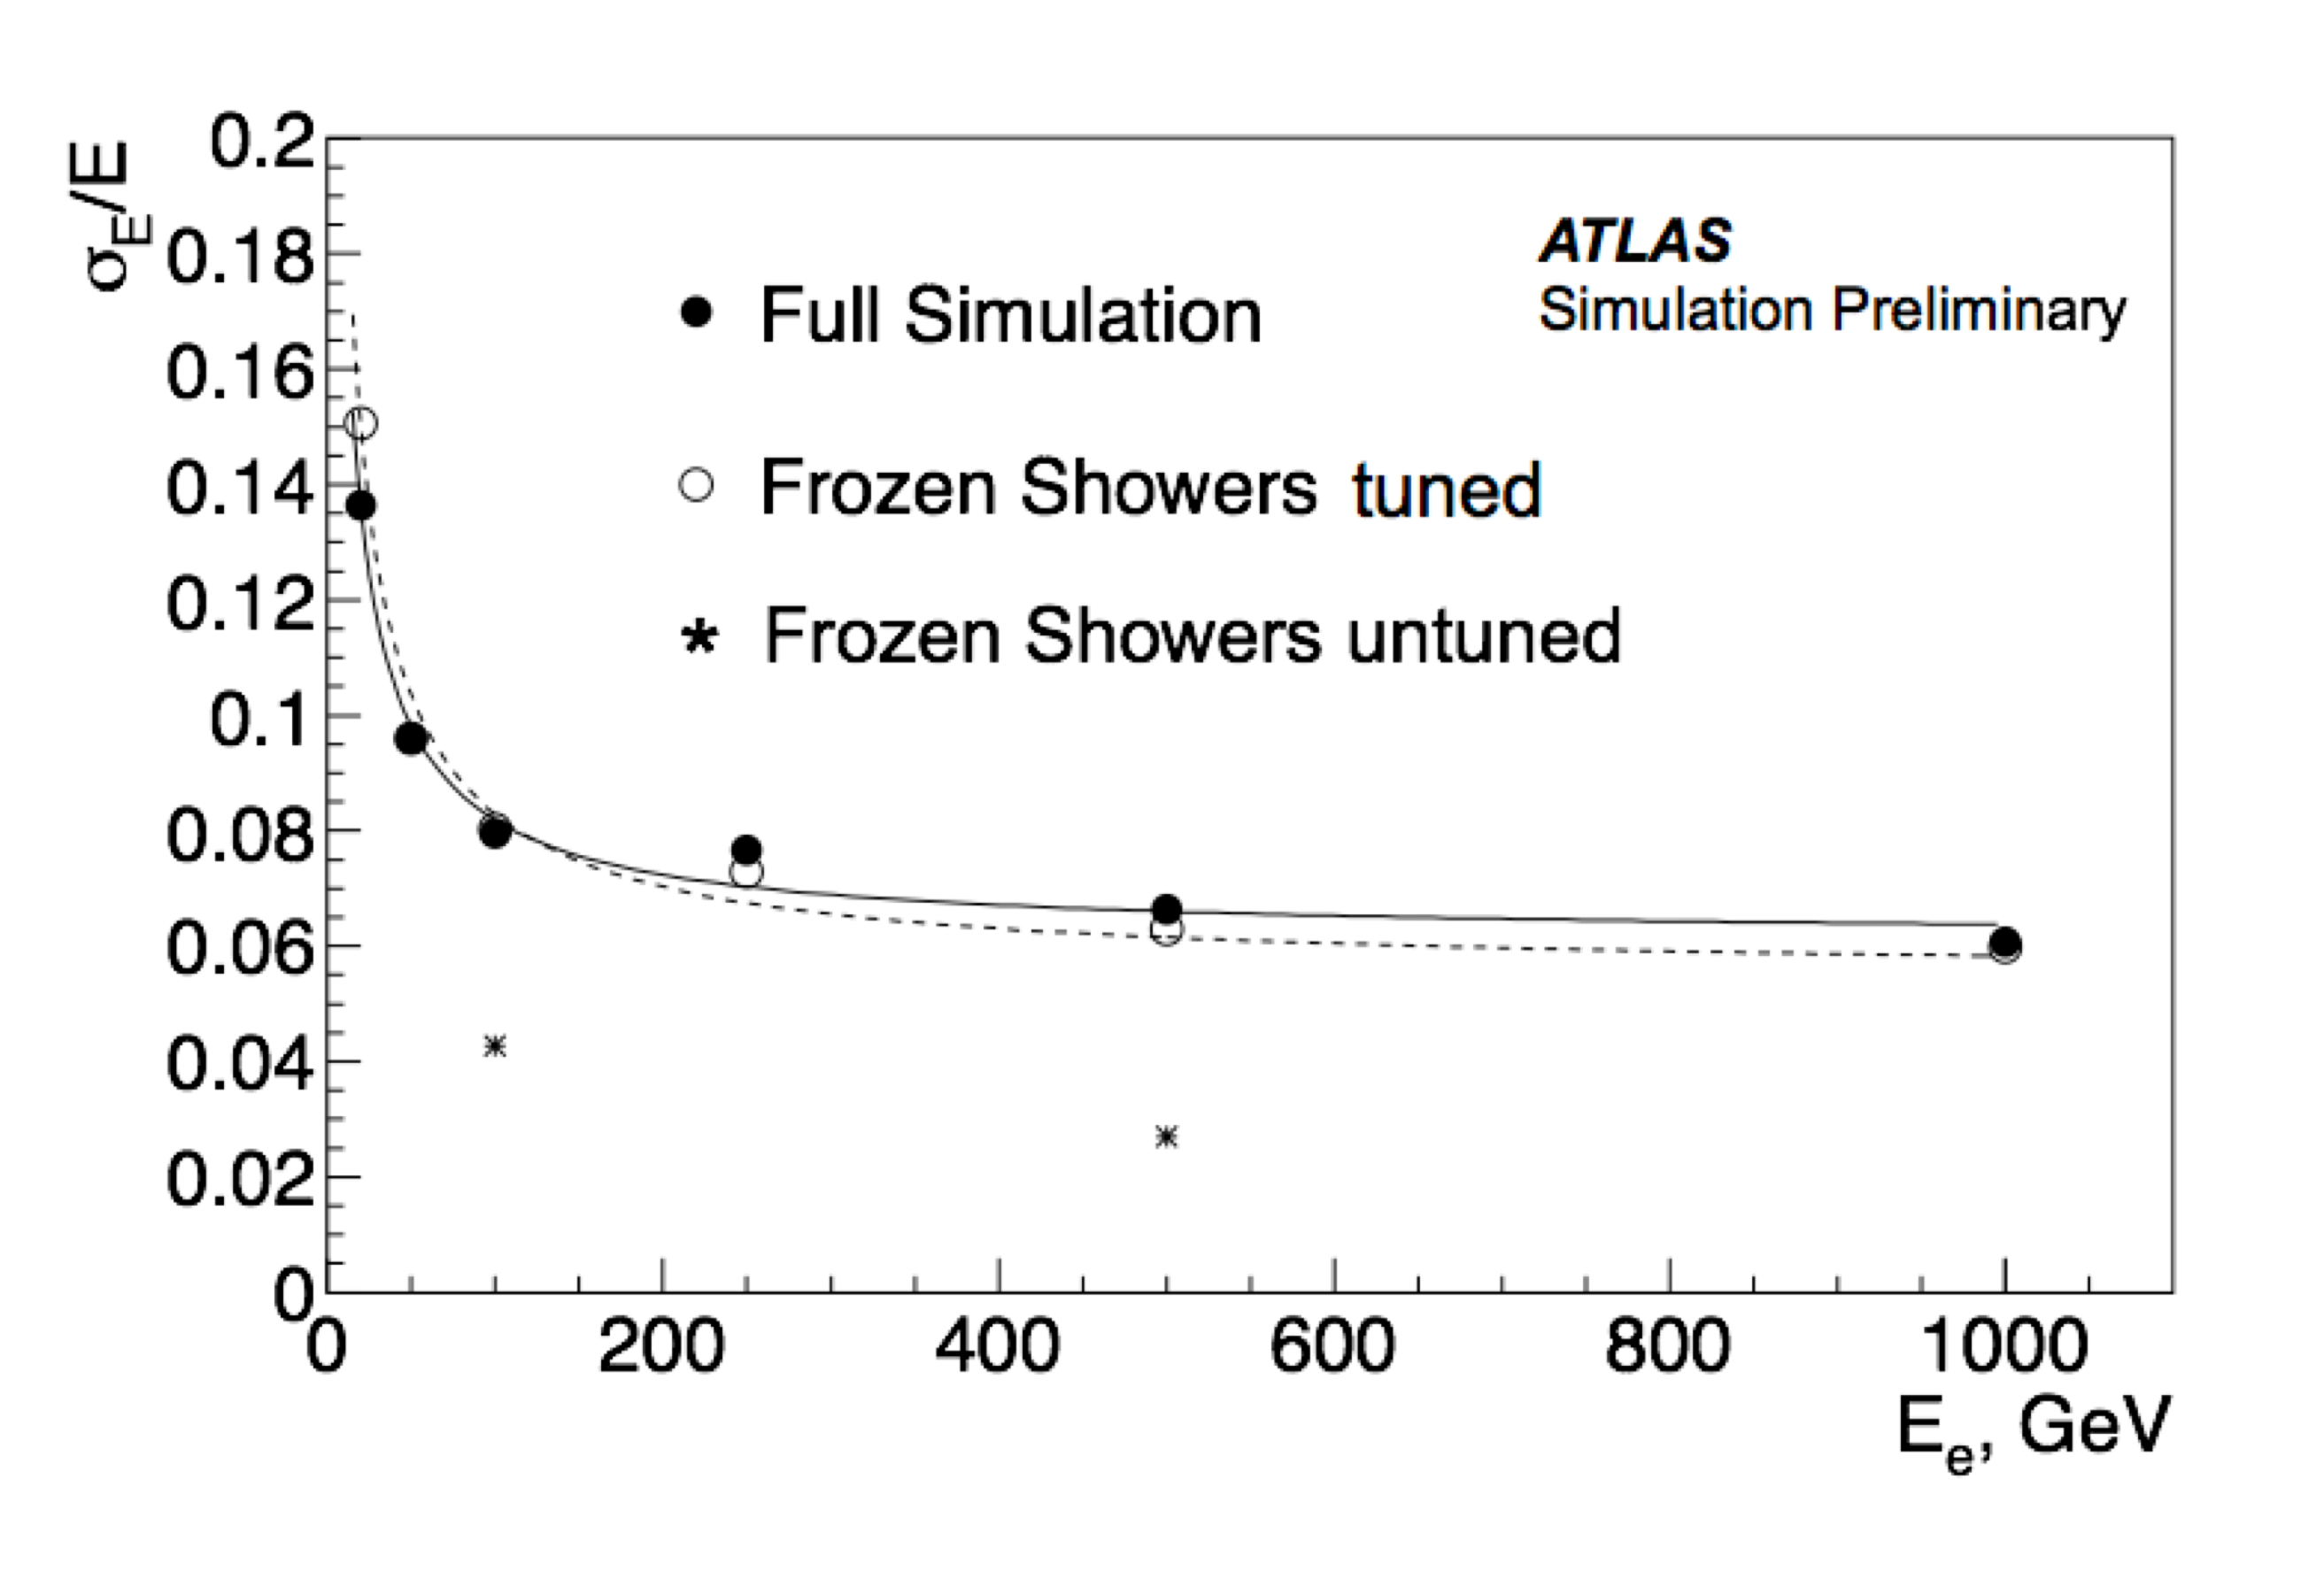
\includegraphics[width=0.8\textwidth]{MC/fs.png}
\caption{Simulated electron resolutions for full simulation (black dots), tuned (white circles) and untuned (star points) Frozen Showers. }
\label{fig:FS_resolution}}
\end{figure}

\section{Machine learning based bin finding procedure}\label{sec:MLBinning}

Since Frozen Showers method is used in the \atlas simulation, there was a need for a more automatic procedure of library generation with proper electron resolution. One of the possible ways is to choose the different positions of liquid argon bins using machine learning tools. In this section, a newly developed automatic bin finding procedure is explained.

\subsection{Machine learning introduction} 

Machine learning is a set of algorithms for finding patterns in the data without being explicitly programmed. There are two main types of machine learning algorithms: \textit{supervised}, where an example of the desired output is provided by the "supervisor" and \textit{unsupervised} , where no labels are given to the algorithm\cite{0070428077}. The initial parameters of interest, which are used in the algorithm to "learn", are called \textit{features}. 

Machine learning algorithms can be used for solving a classification problem, where each event should be identified to one of the specified classes. In this analysis, decision trees and support vector machines from \cite{scikit-learn} are used. 

\subsubsection{Binary decision trees}

\textit{Binary decision trees}\cite{cart84-2} (also called single decision trees) are one of the most commonly used machine learning algorithms for classification problems in particle physics. These algorithms can be represented as a set of sequential selections on input variables. The advantages of these algorithms are the simplicity of visualization and interpretation. 
Example scheme of this algorithm is shown in Fig.~\ref{fig:MLAlgo} a). Red circles indicate the nodes of the tree. Each node corresponds to one of the internal input variables and connects to two branches, which are split by the decision on the value of selected variable. The first node is called a root node. The depth of the tree is defined as the number of branches from the root node to the given node. A tree ends with squares, called leaf nodes, where all events are classified into a particular class. The tree, where each node has at most two branches is called binary decision tree.

A binary tree is build using the variable called Shannon entropy\cite{ShannonEntropy}, which is defined similarly to the entropy in physics:
\begin{equation}
S=- \sum_{i=1}^{N} p_i log_2 p_i.
\end{equation}
Here $p_i$ is the probability to find an event of class $i$. The information gain is defined as:
\begin{equation}
IG(Q) = S_0 - \sum_{i=1}^{2}S_i,
\end{equation}
where $S_0$ is the initial entropy (without new node), $S_i$ is the entropy of the one of the $i$-th branch of the node. From all of the possible variants of splits, the one with the highest information gain is taken. 

\subsubsection{Support vector machines}

\begin{figure}[!tbp]
\begin{minipage}[h]{0.49\linewidth}
\center{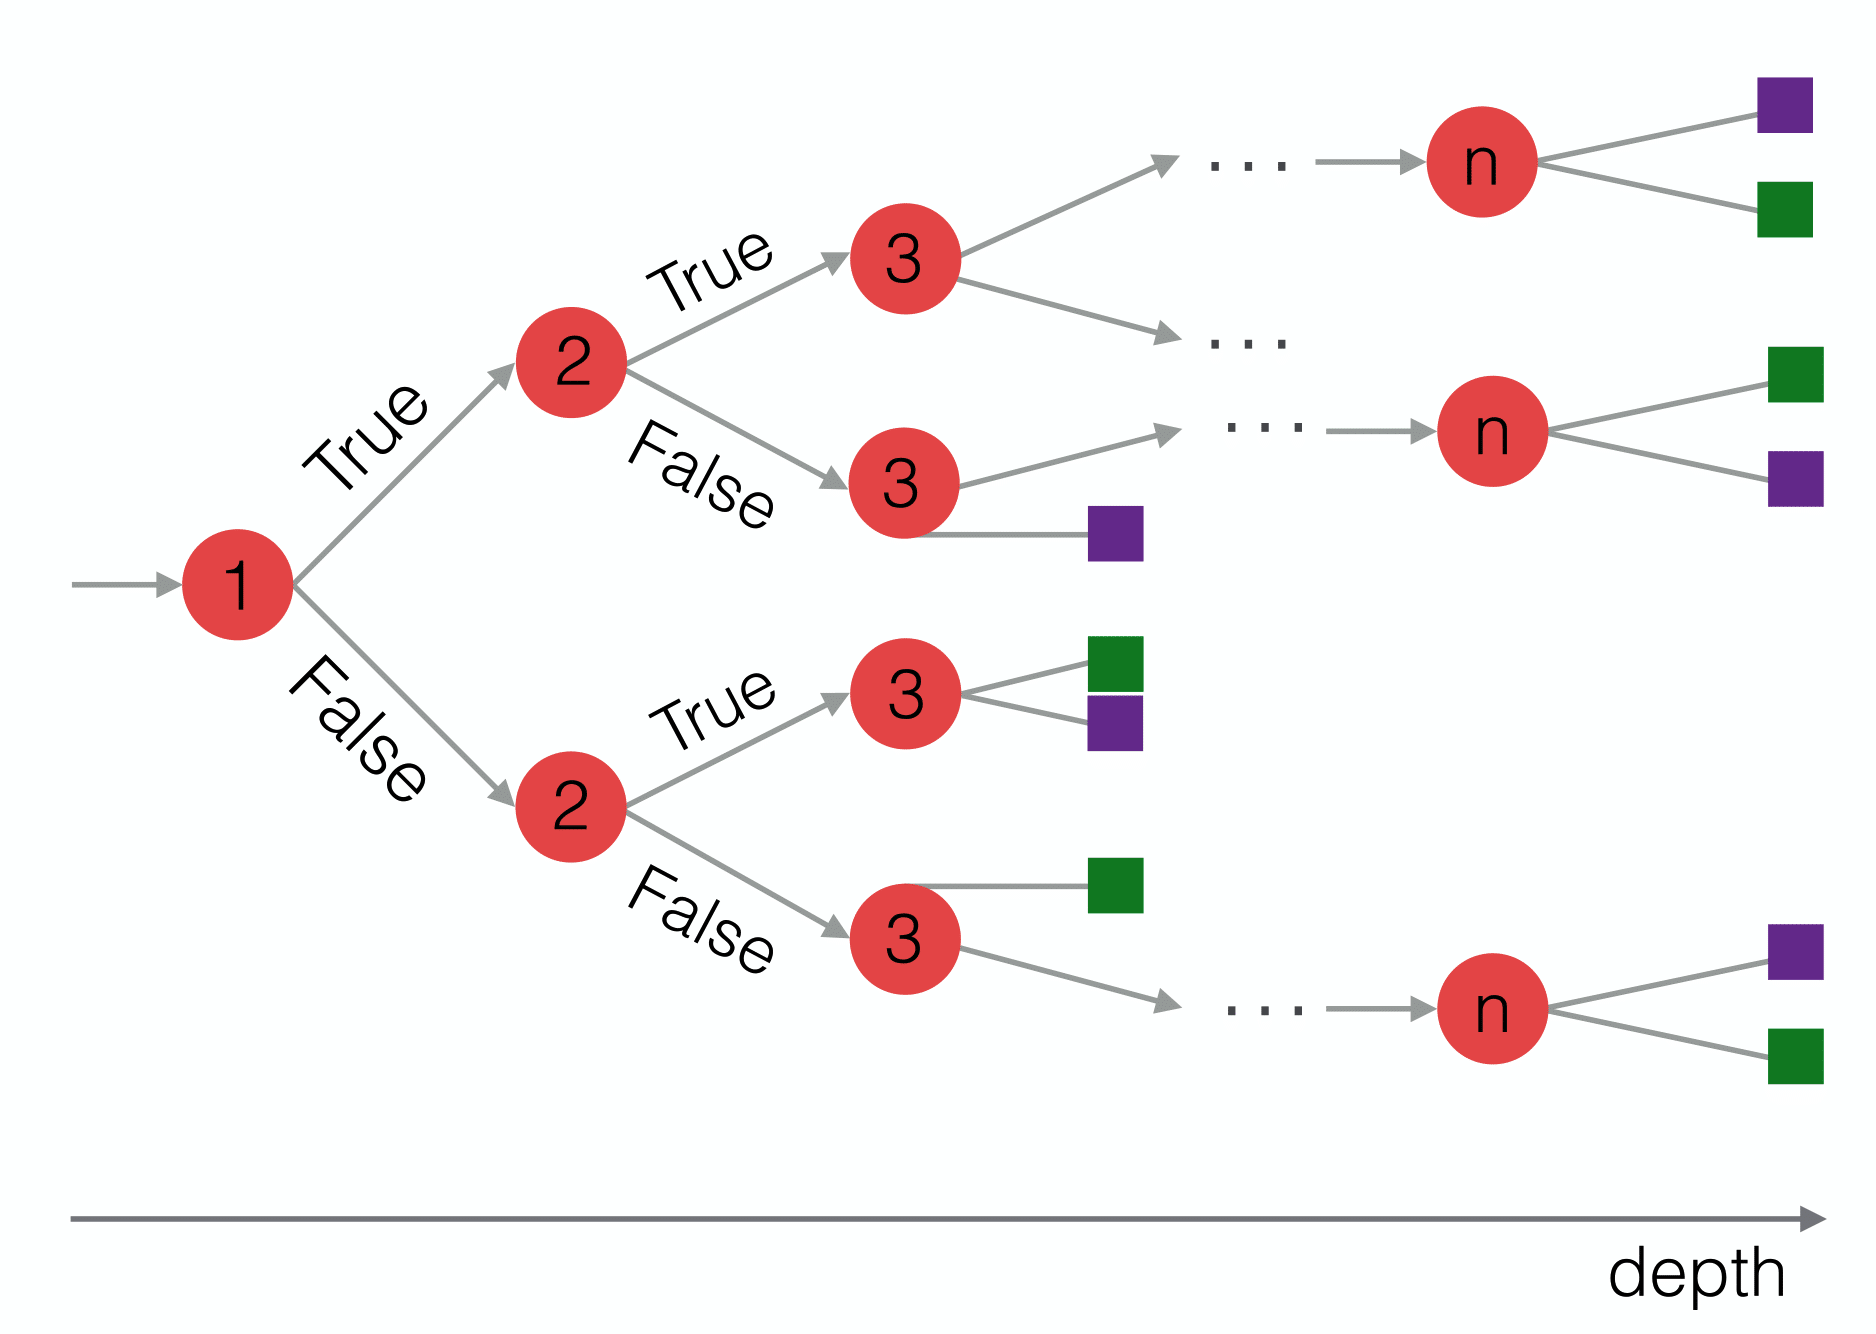
\includegraphics[width=1.\linewidth]{MC/DecisionTree.png} \\ a)}
\end{minipage}
\hfill
\begin{minipage}[h]{0.49\linewidth}
\center{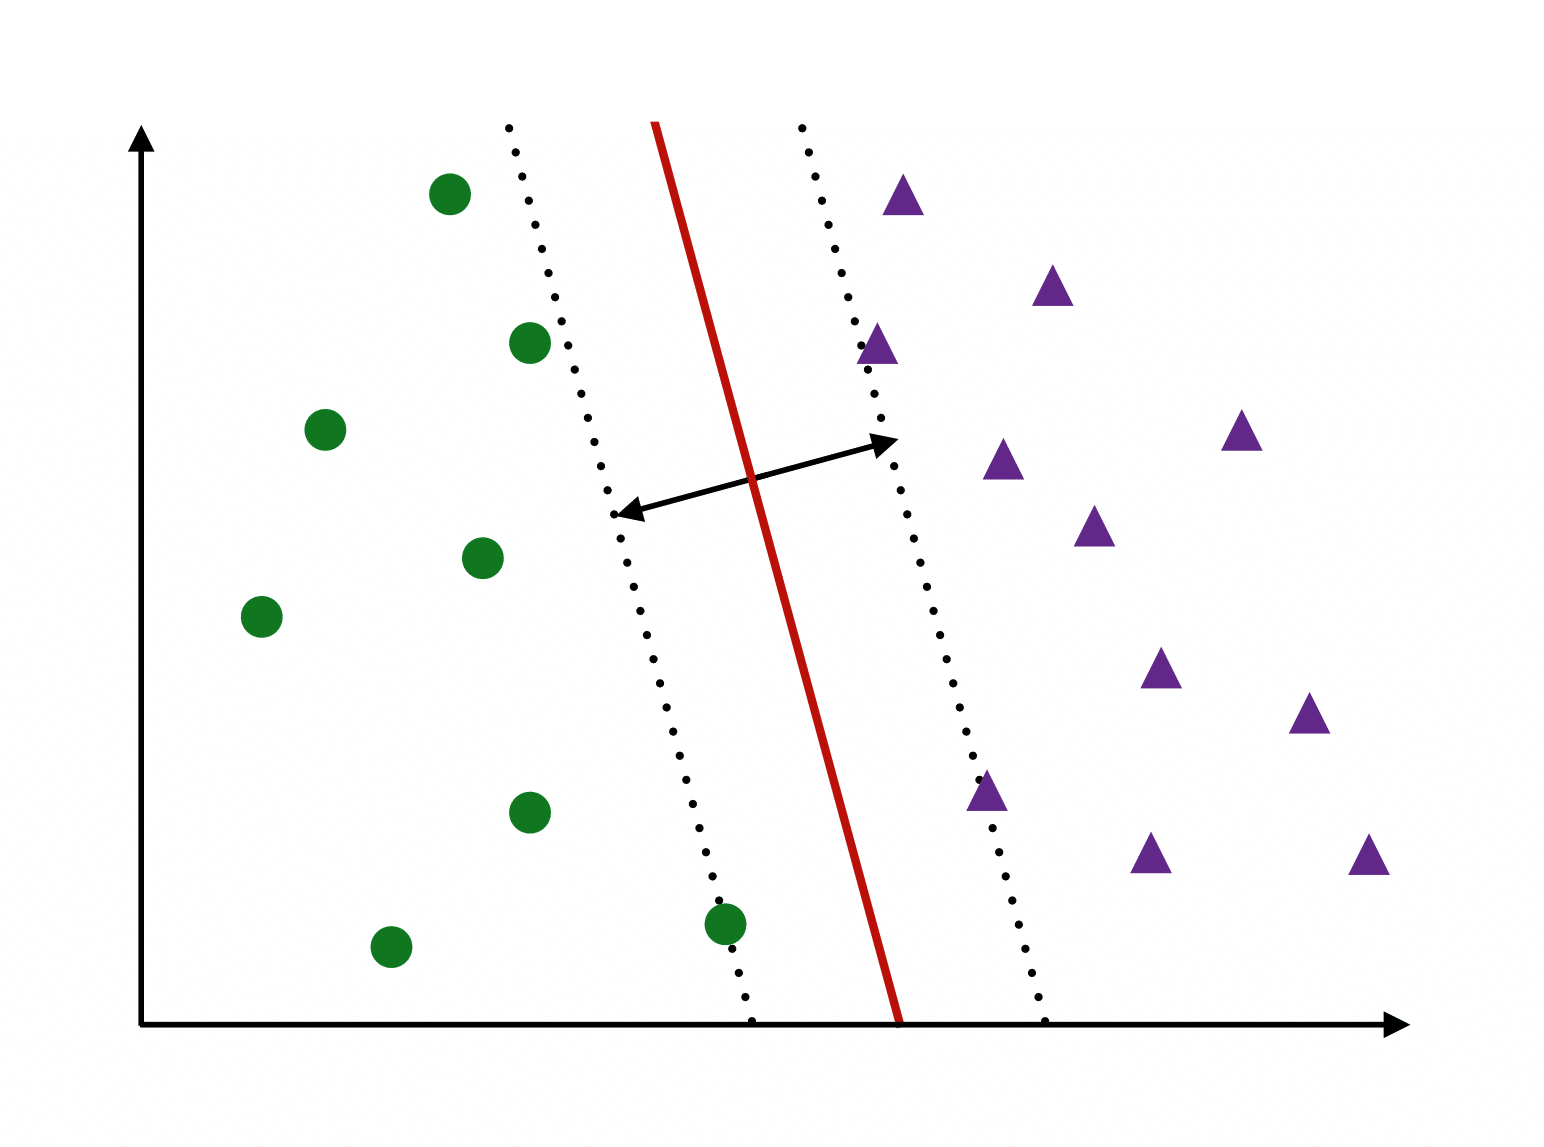
\includegraphics[width=1.\linewidth]{MC/SVM.png} \\ b)}
\end{minipage}
\caption{Schematic representation of machine learning algorithms, used in this analysis for the classification of showers. Green  and violet figures represent the two classes of events.
a) Representation of a binary decision tree structure: red circles correspond to nodes. Each node has two branches that are split by the decision on the value of selected variable. Squares represent "leafs", where events are classified are classified into a particular class.
b) Representation of the SVM algorithm. The solid line shows the dividing hyperplane. The dashed lines represent the maximum margin boundaries.}
\label{fig:MLAlgo}
\end{figure}

\textit{Support vector machines} (SVM)\cite{VapLer63} is a machine learning algorithm which can be used for classification problems. In this algorithm, each event is represented in a $p$-dimensional parameter space. The classification is performed by finding a hyperplane that separates two given classes with the largest separation (Fig.~\ref{fig:MLAlgo} b). The hyperplane can be described using the set of points $\vec {x}$ in the parameter space satisfying the relation:
\begin{equation}
\vec{w}\cdot \vec{x} - b = 0,
\end{equation}
where $\vec{w}$ is a vector normal to the hyperplane and the parameter $\frac {b}{\|{\vec {w}}\|}$ determines the offset of the hyperplane from the origin along the normal vector $\vec {w}$. 

The maximum margin boundaries between two classes are described by equations:
\begin{eqnarray}
\vec{w}\cdot \vec{x} - b = 1, \\
\vec{w}\cdot \vec{x} - b = -1,
\end{eqnarray}
where $\frac{2}{\|\vec{w}\|}$ is the distance between these 2 hyperplanes. The planes with the maximum margin between them correspond to the minimum $\|\vec{w}\|$. 

In order to prevent each point from falling into the margin, the following constrain should be satisfied: 
\begin{eqnarray}
\vec{w}\cdot \vec{x} - b \geqslant 1 (\textrm{ where } y_i = 1),\\
\vec{w}\cdot \vec{x} - b \leqslant -1 (\textrm{ where } y_i = -1),
\end{eqnarray}
where $y_i$ represents the class of the $i$-th event, classified as 1 or -1. These equations can be rewritten as:
\begin{equation}
y_i(\vec{w}\cdot \vec{x} - b ) \geqslant 1.
\end{equation}

It is also possible to construct a non-linear classifier by replacing the dot-product with a different kernel function. In this analysis, different kernel functions have been tested and the best performance was obtained using the radial basis function (RBF) kernel, defined as:
\begin{equation}\label{eq:RBF}
K_{rbf}(\vec{x}_i, \vec{x}_j) = e^{-\gamma | \vec{x}_i - \vec{x}_j|^2} \, \gamma >0,
\end{equation}
where the parameter $\gamma$ adjusts the width of the kernel.




\subsection{Electron shower categorization}

\begin{figure}[!tbp]
\center{
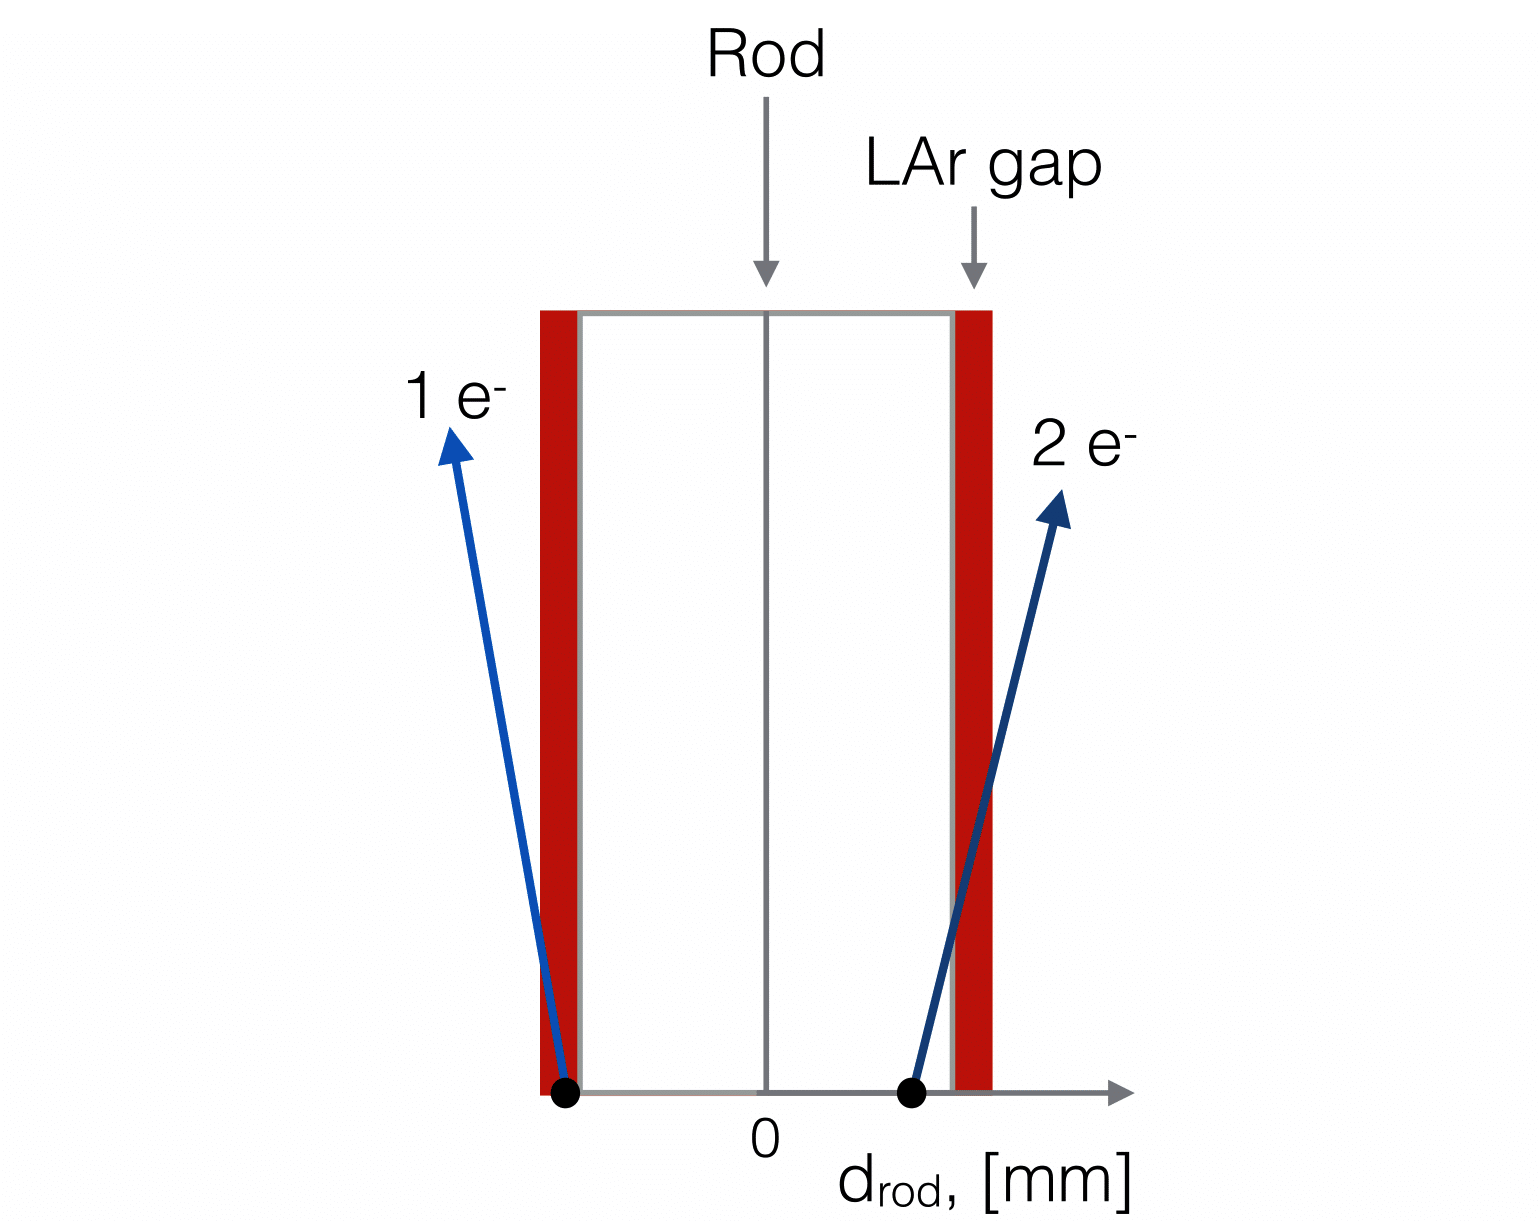
\includegraphics[width=0.5\textwidth]{MC/Model2.png}
\caption{Schematic representation of the model of shower creation in the FCAL. Electron 1 is created in a liquid argon gap. Electron 2 is created near a liquid argon gap and crosses the gap. This causes a smearing of shower distribution. Electrons created in the sensitive material tend to create more energetic showers than electrons produced in the dead material. }
\label{fig:Model}}
\end{figure}

The FCAL modules consist of different types of material and therefore showers produced inside the dead material are usually having lower energies than those created in sensitive material. However, the validation (summarized in Fig.~\ref{fig:FS_resolution}) can be interpreted as an implication of high-energy showers production outside the liquid argon gap. This can be explained by the fact that electrons, created in a dead material, can cross a liquid argon gap (and give a hit) as shown in Fig.~\ref{fig:Model}. These electrons would be indistinguishable from electrons created directly in the sensitive material (electron 1 in Fig.~\ref{fig:Model}).  Due to this similarity, electrons created outside the sensitive material can be combined in one class of the \textit{sensitive material showers}. Showers that did not cross a liquid argon gap, are called \textit{dead material showers}.  The real gap position in this model is substituted by the \textit{effective liquid argon gap}, which has a larger width.

The width of the effective liquid argon gap depends on the following parameters:
\begin{description}
\item [Electron energy] The gap should get wider with higher energy of the initial electron, because of the growth of the mean free path of electron with energy;
\item [Direction of the electron] Electrons aligned collinearly with the liquid argon gap will have a smaller probability to cross it. This probability will grow with the angle (with reaching its maximum at  $90^{\circ}$).
\end{description}

The procedure of finding the effective liquid argon gap is divided into two steps:  in the first step the showers are classified using the simulated parameters of the showers, in the second step the dividing hyperplane in  $d_{rod}$ and $E$ phase-space is produced. The training sample and classifiers used in this two steps are discussed in the following subsections.

\subsubsection{Training sample}

The parameters of electrons, substituted by the frozen showers, have a complicated structure and depend on the physics processes. Machine learning algorithms could identify these dependencies instead of the position of the width of the effective liquid argon gap, so the simplified training sample is used. The training sample was produced by simulation of electrons produced in the FCAL. 

Fig.~\ref{fig:EtaMomVsEnergy} shows the distribution of the shower direction ($\eta^{direction}$) vs electron energy for electrons used in the simulation of 1 TeV electron. Most of the showers are produced in the $\eta$ range between 3.0 and 5.0, which corresponds to the coordinates of the FCAL. The direction of the shower is highly correlated with the position of the electron. Therefore, electrons were generated uniformly in $\eta$ between 3.0 and 5.0. In order to treat equally high and low energy electron initial showers, a uniform distribution of the electron energies is used.

\begin{figure}[!tbp]
\center{
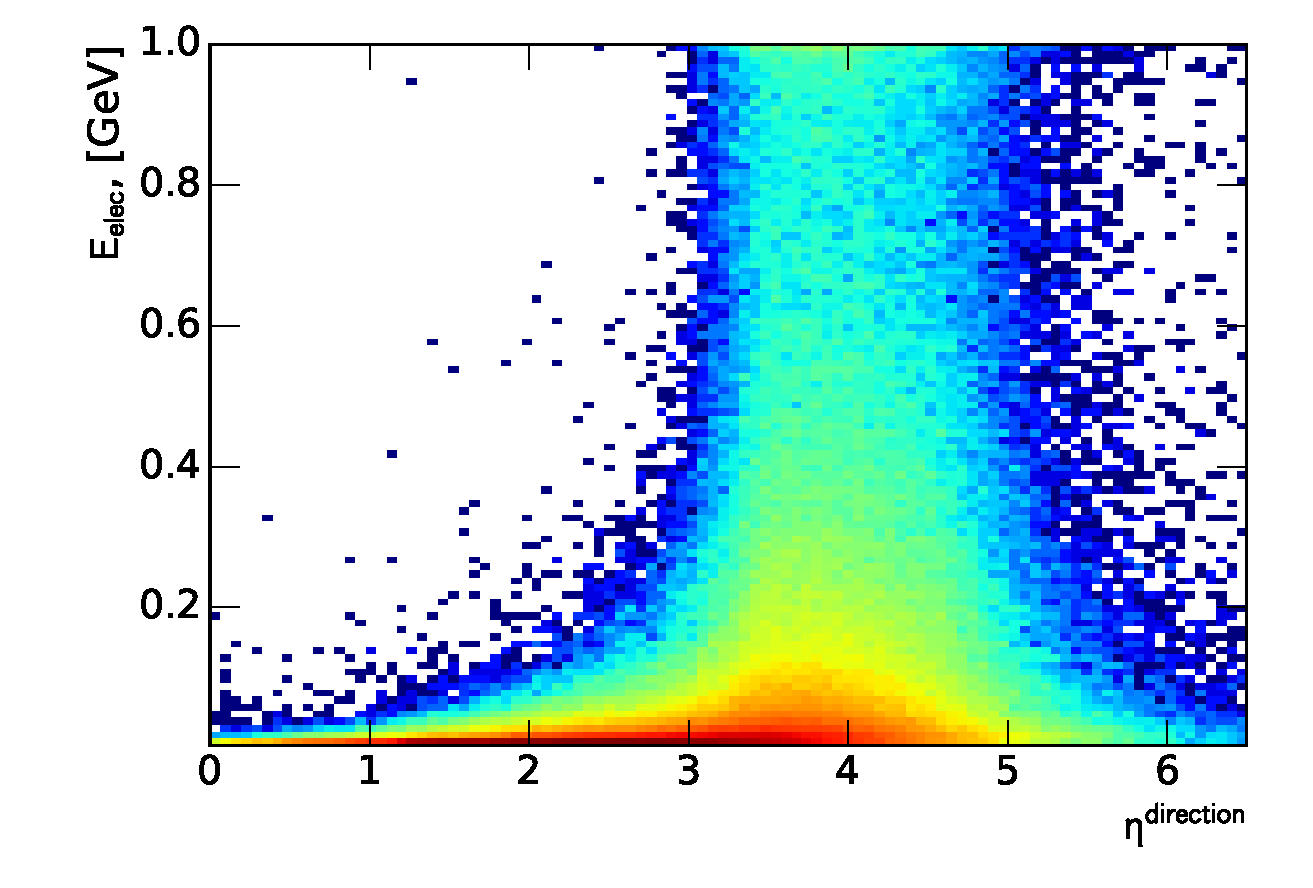
\includegraphics[width=0.8\textwidth]{MC/FSEtaMomVsEnergy.pdf}
\caption{Distribution of sub-shower energy vs direction of a shower ($\eta$) for showers used in the production of 1 TeV electrons.}
\label{fig:EtaMomVsEnergy}}
\end{figure}

\subsubsection{First classifier}

The first classifier aims to categorize all showers using the simulated parameters. A supervised learning algorithm is used on artificially reduced pre-labeled training sample. The results obtained can be expanded to the full sample afterward. 
 
The pre-labeling procedure uses the definitions of sensitive and dead material showers (Fig.~\ref{fig:SchemePresel}). Showers, produced in the liquid argon gap are labeled as the sensitive material showers. Showers, produced near the rod center and on the edges of the cell are labeled as dead material showers due to the small probability of the initial electrons to cross the liquid argon gap. For this classifier, simple decision trees have been chosen since it has shown an excellent classification efficiency on the reduced training sample. Different input parameters have been tested using variance. The best differentiating parameters are:
\begin{itemize}
\item Total shower energy, defined as the sum of all sensitive material hits energies in the shower;
\item Maximum hit fraction, calculated as the energy of the most energetic hit divided by the total shower energy;
\item RMS of the hits, calculated as the standard deviation of the hits energies in the shower.
\end{itemize}
The classification efficiency of the obtained binary search tree for the reduced sample is 97\%. The results expanded to the full phase space are shown in Fig.~\ref{fig:Class} a). 

\begin{figure}[!tbp]
\center{
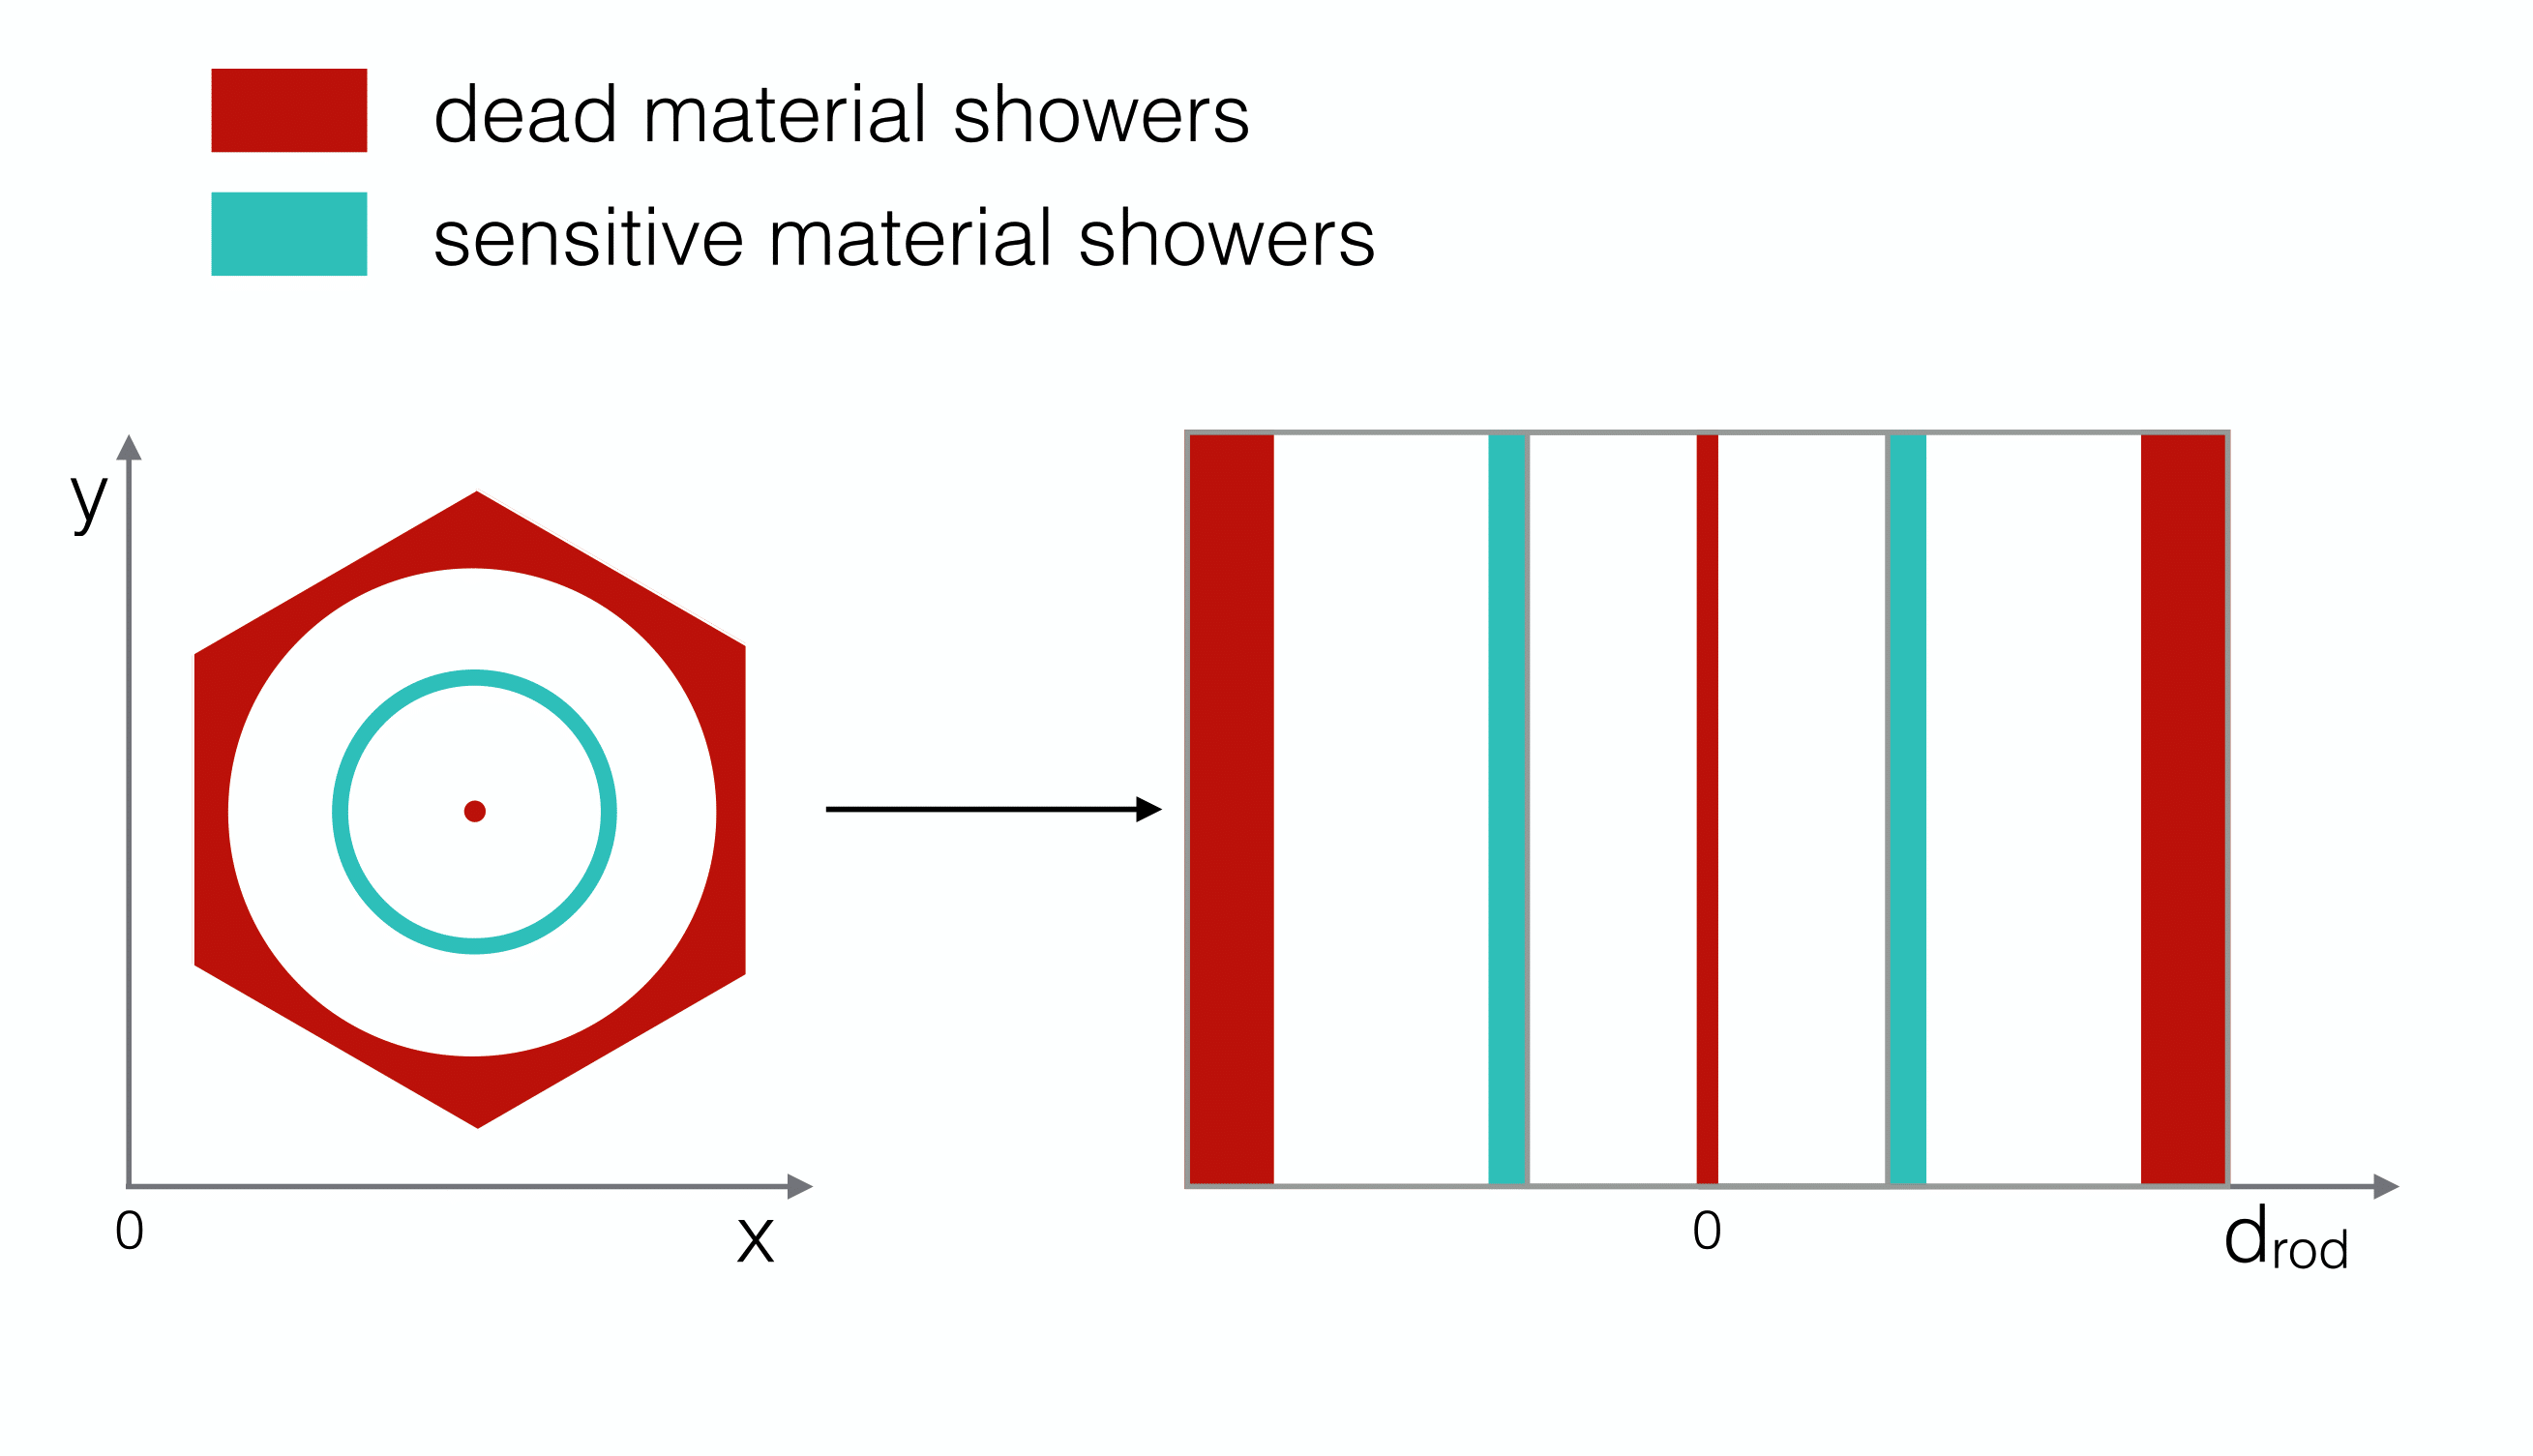
\includegraphics[width=1.0\textwidth]{MC/FirstClassifierData.png}
\caption{Schematic representation of the preselected data for the first classifier in the x-y (left) and distance (right) plane. Electrons, created near the rod center and on the borders of the module have low probability to cross the sensitive material, while those created inside the liquid argon gap are considered as sensitive material showers.}
\label{fig:SchemePresel}}
\end{figure}

\subsubsection{Second classifier}

\begin{figure}[!tbp]
\begin{minipage}[h]{0.49\linewidth}
\center{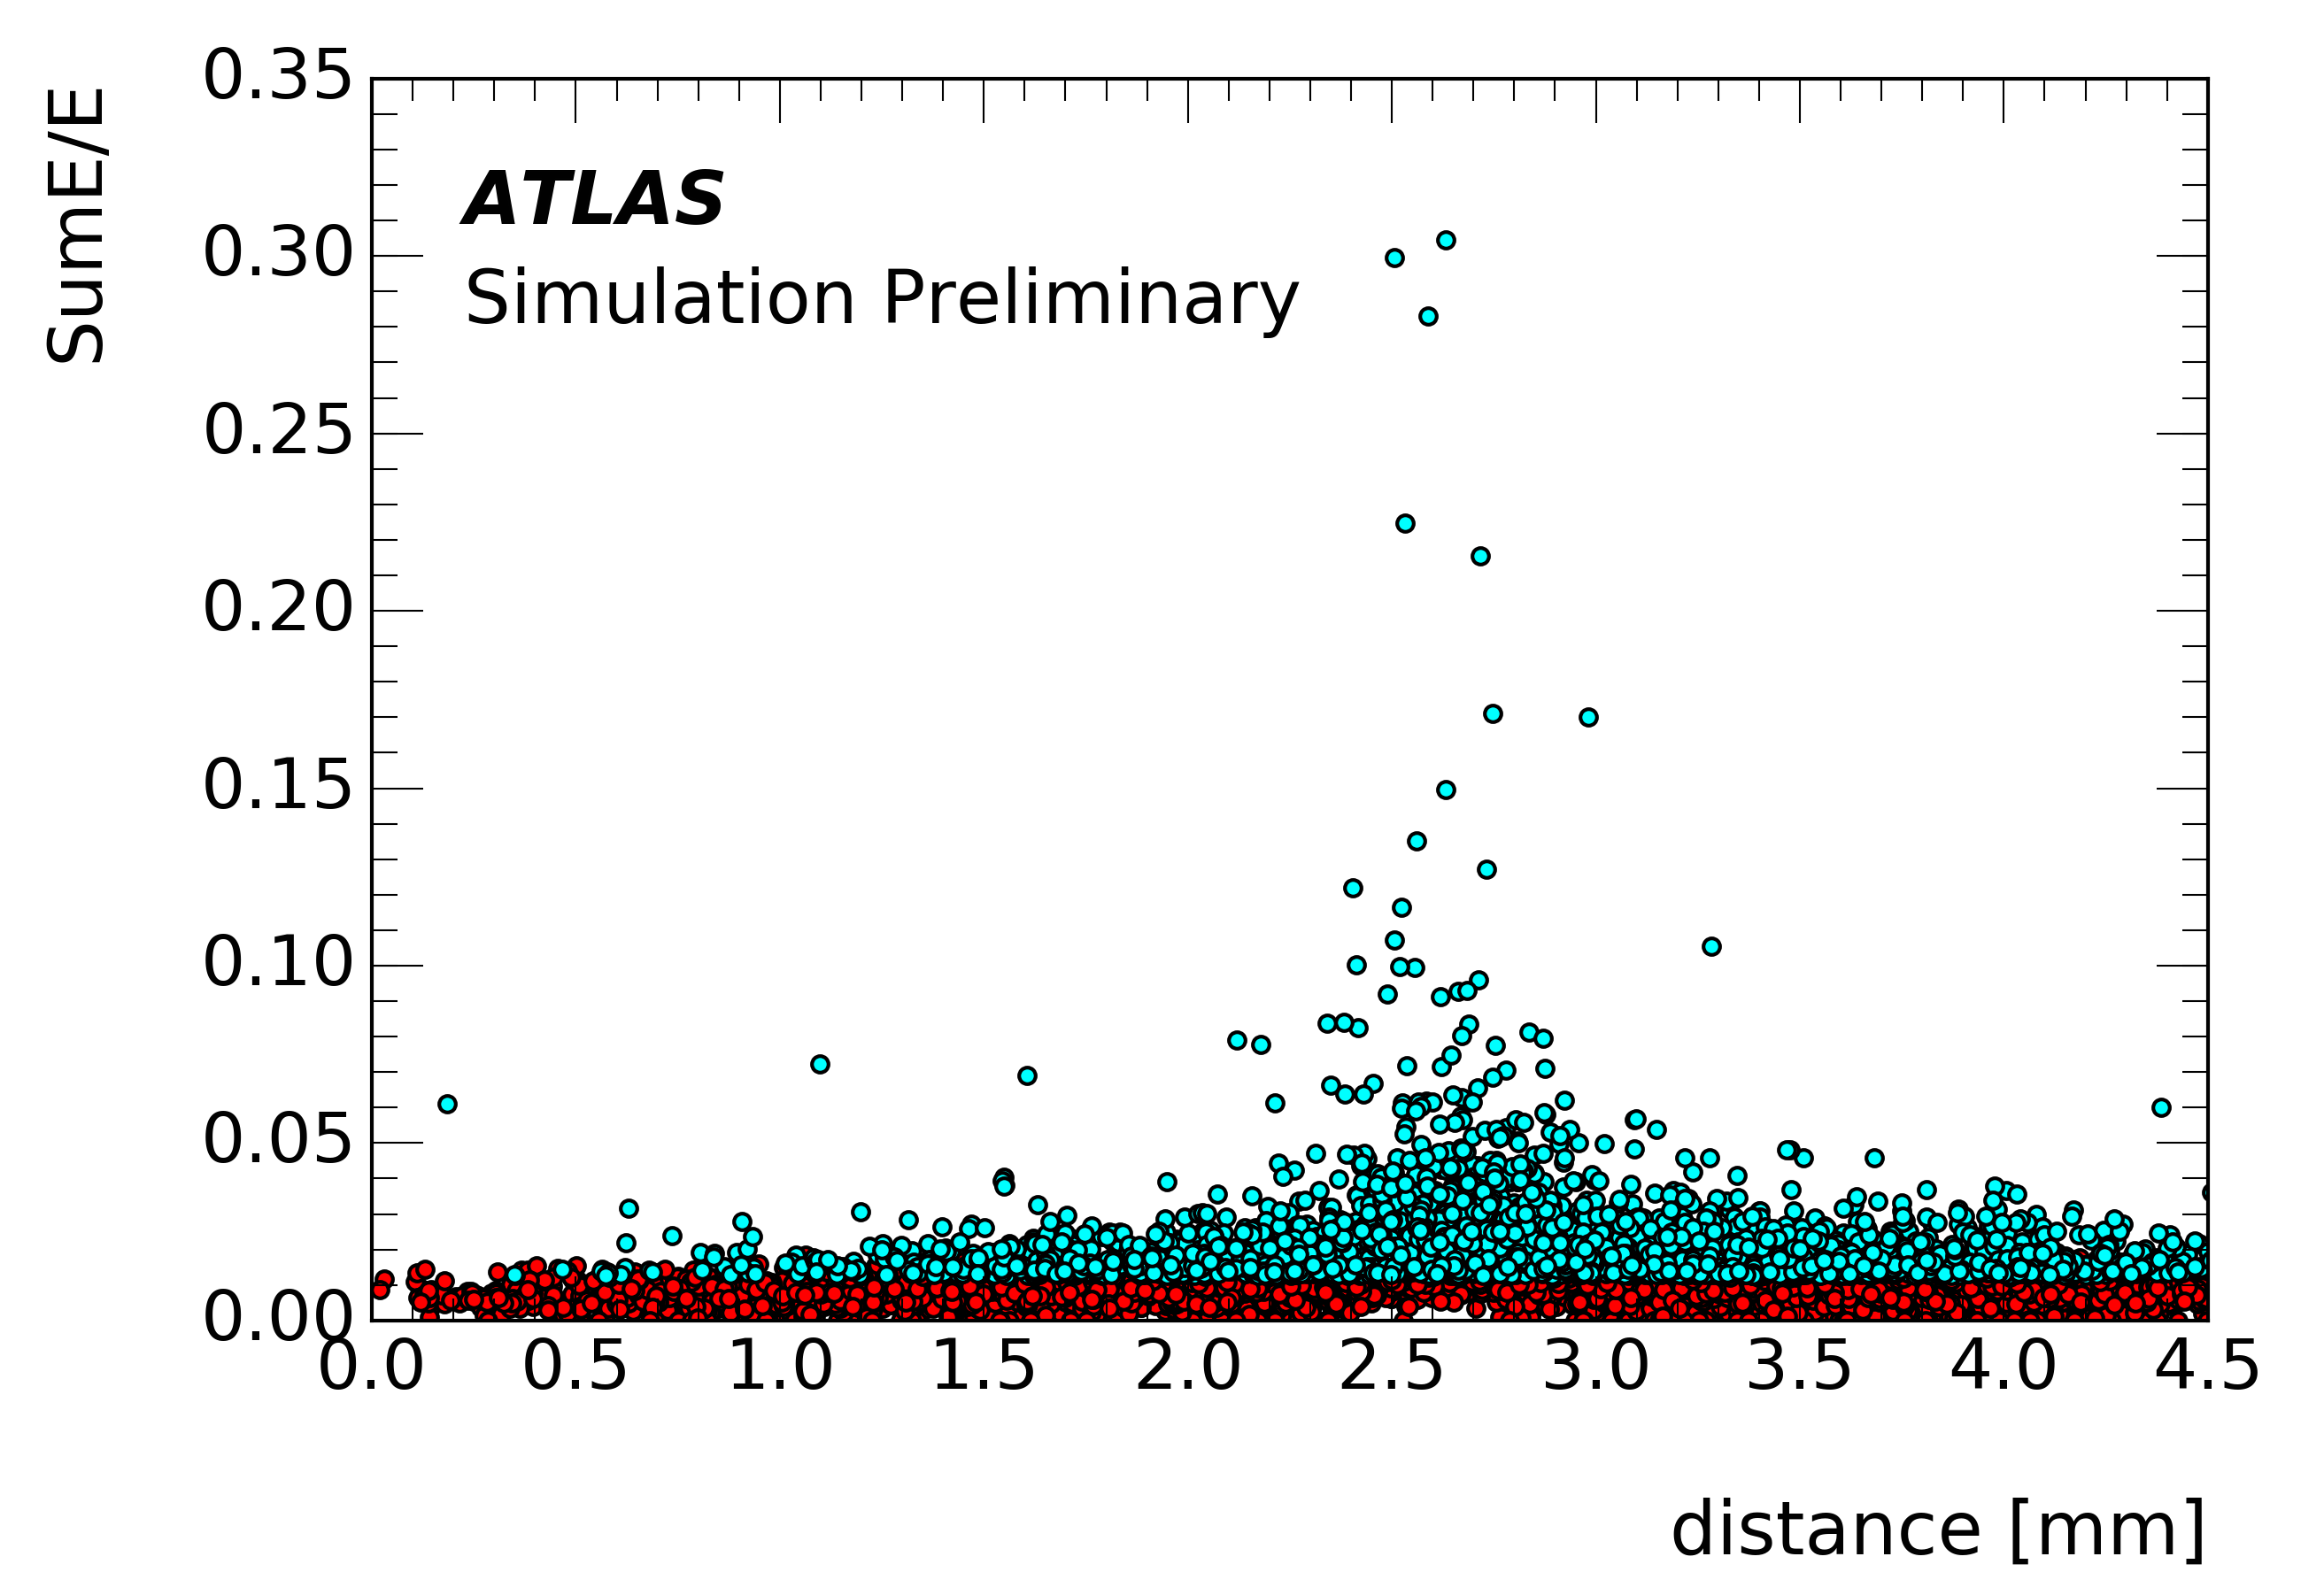
\includegraphics[width=1.\linewidth]{MC/firstClassifier.png} \\ a)}
\end{minipage}
\hfill
\begin{minipage}[h]{0.49\linewidth}
\center{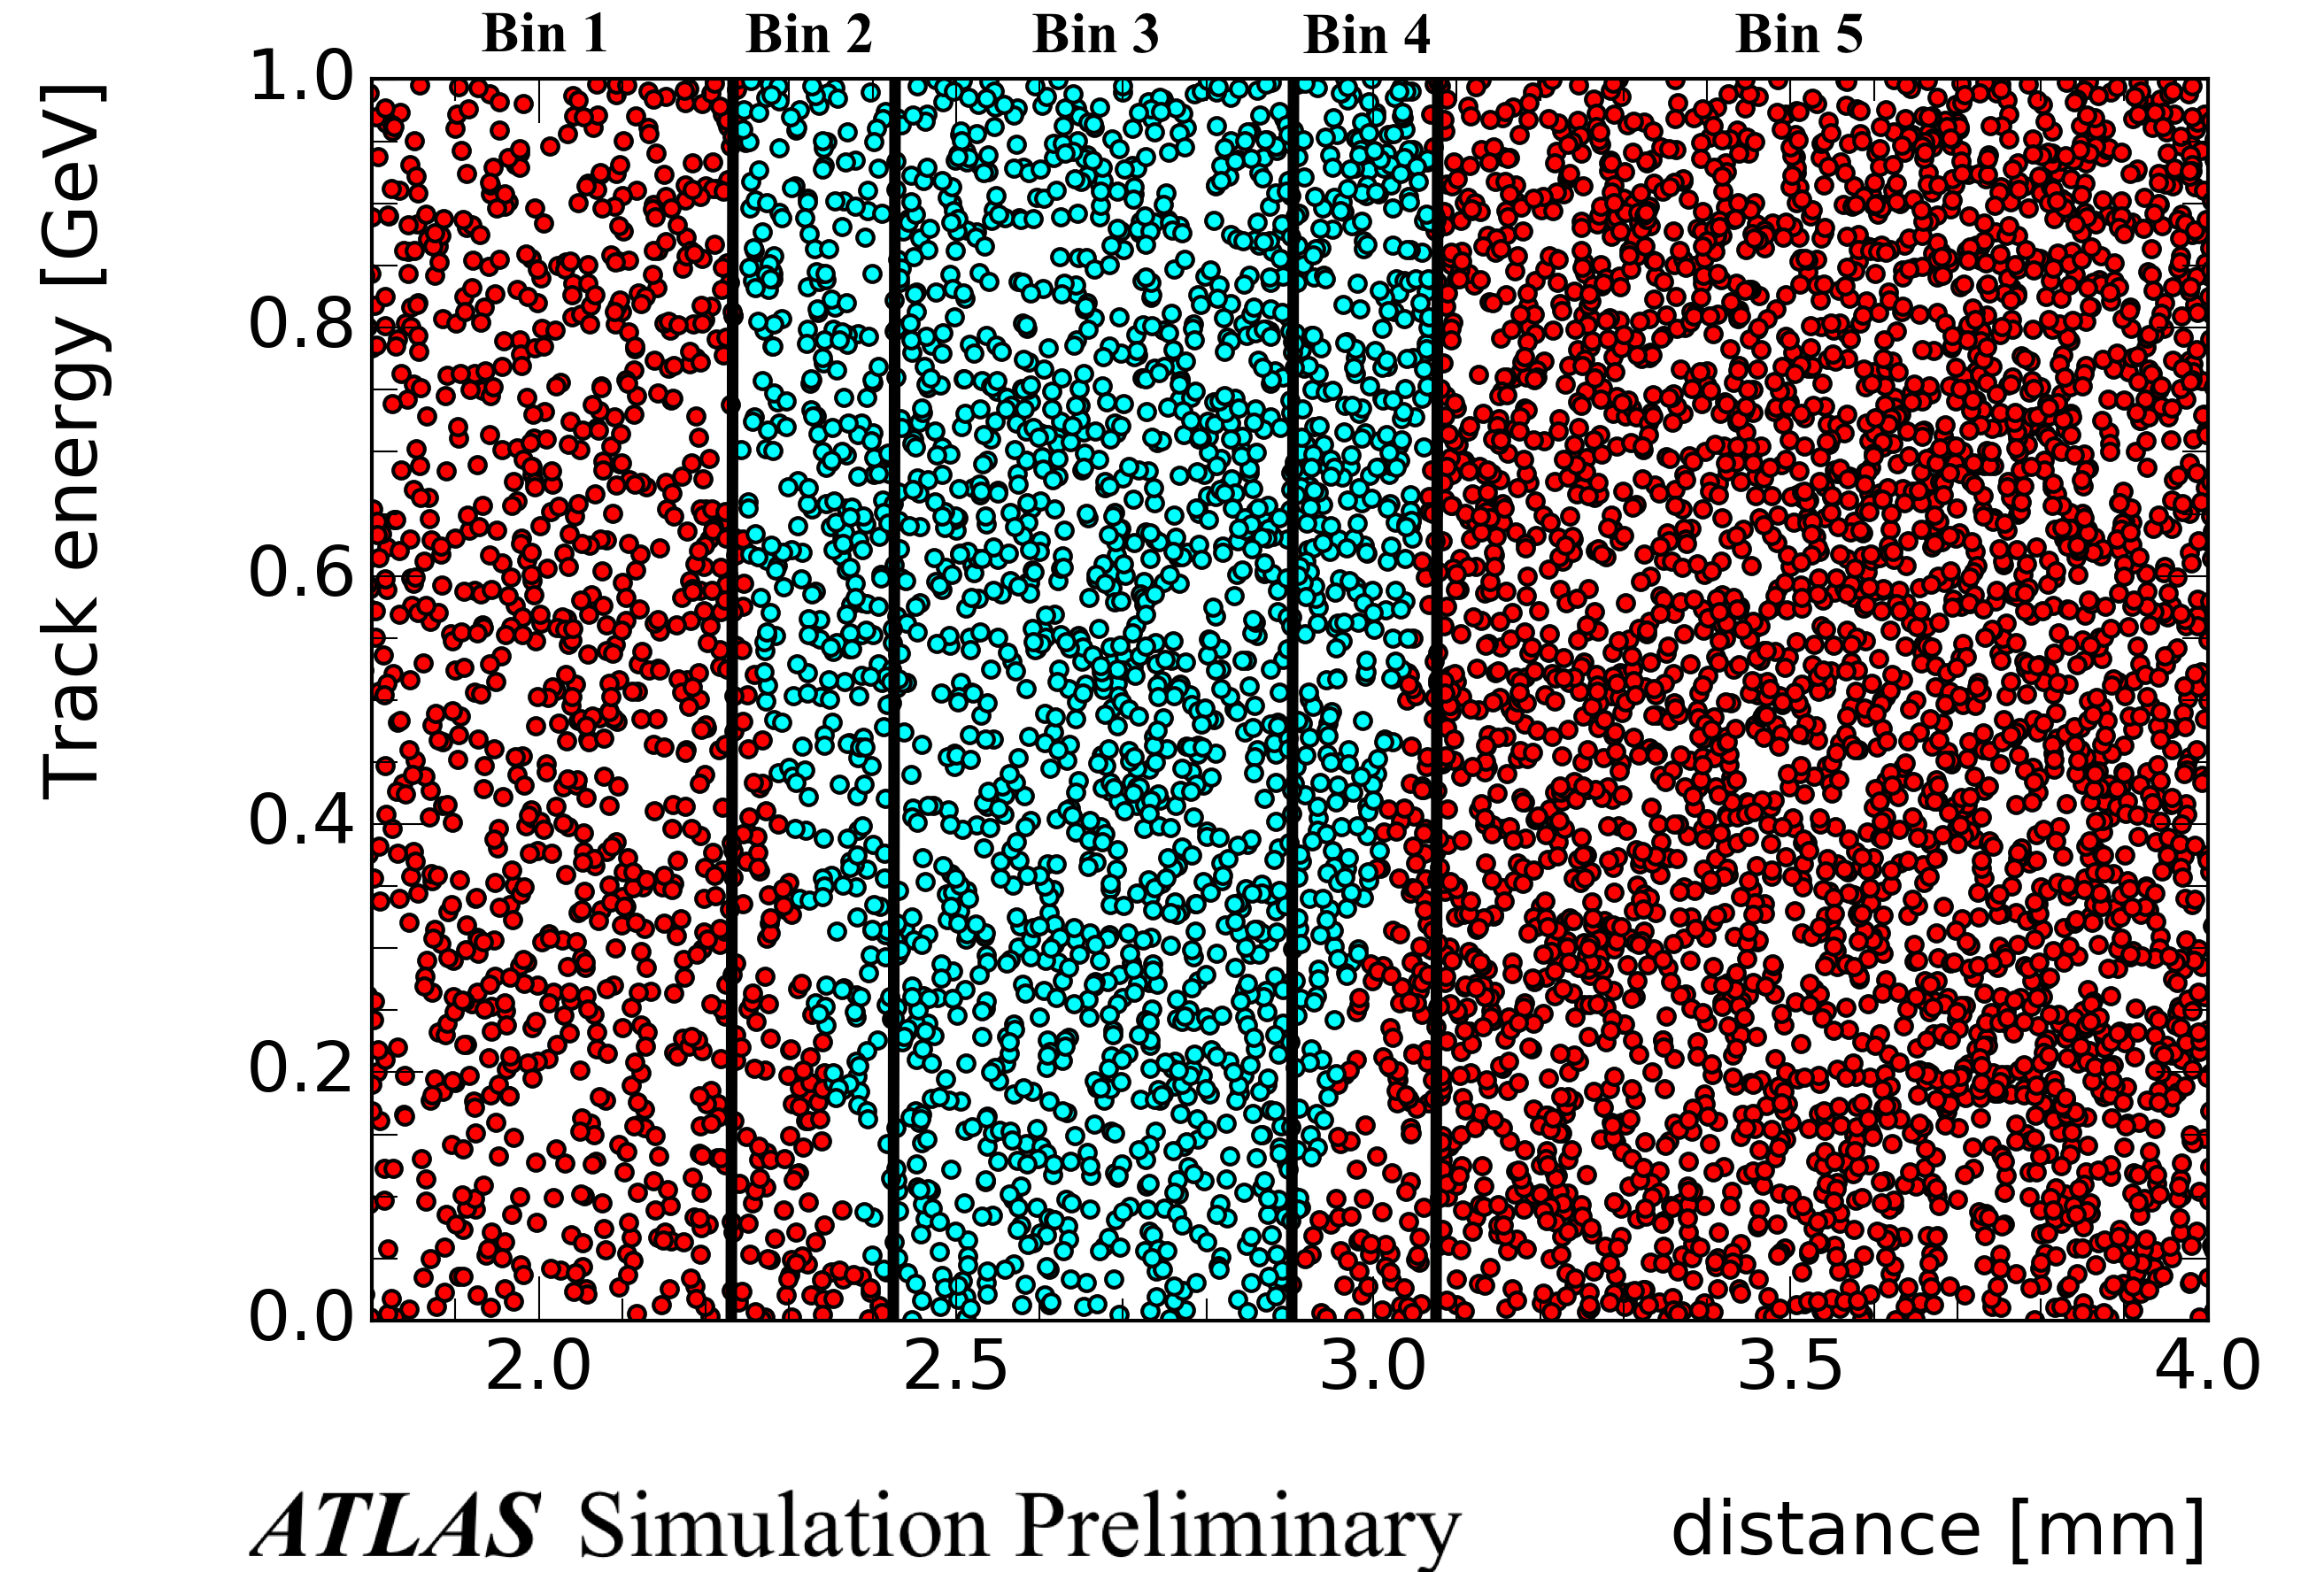
\includegraphics[width=1.\linewidth]{MC/secondClassifier.png} \\ b)}
\end{minipage}
\caption{Results of machine learning algorithm classification for a) first classifier and b) second classifier. Cyan dots correspond to sensitive material showers, red to dead material showers. The black lines in Fig. b correspond to the resulting bin positions.}
\label{fig:Class}
\end{figure}

The second classifier uses predictions of the first classifier as an input. The algorithm reconstructs a hyperplane between two types of the shower using SVM.  As an input it uses the truth parameters of the electron, e.g. energy of the initial electron and its distance to the closest rod center and RBF as a kernel function.  A classification is performed separately in each $\eta$ bin used in the library. 

An example of the classifier output is shown in Fig.~\ref{fig:Class} b). The obtained gap positions are wider than the original ones, as  expected from the model.  The difference between obtained effective liquid gap widths for different $\eta$ bin used in the library is considered to be small. The mean effective liquid argon gap width is used as an input for the bin finding procedure.  

\subsubsection{Interpretation of results}

\begin{figure}[!tb]
\begin{minipage}[h]{0.49\linewidth}
\center{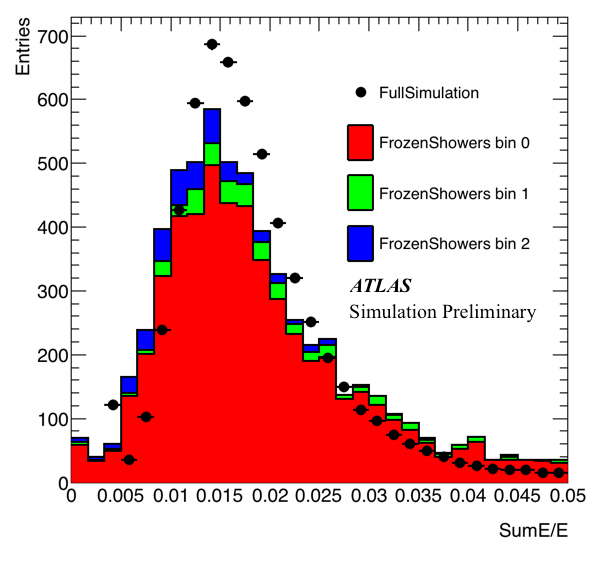
\includegraphics[width=1.\linewidth]{MC/oldSumE.png} \\ a)}
\end{minipage}
\hfill
\begin{minipage}[h]{0.49\linewidth}
\center{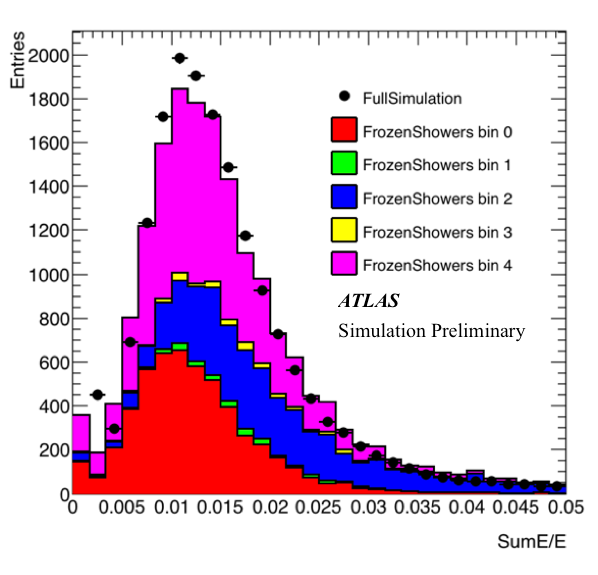
\includegraphics[width=1.\linewidth]{MC/newSumE.png} \\ b)}
\end{minipage}
\caption{Comparison of the distributions of shower energy divided by  the energy of the initial electron between full simulation and toy MC for a) old "tuned" libraries with 1 liquid argon gap bin and b) new libraries using 3 liquid argon gap bins. There are still remaining differences between full simulation and toy MC, but the new machine learning binning gives a better agreement with full simulation.}
\label{fig:Interpret}
\end{figure}

The resulting hyperplane from the second classifier can be translated to the bin positions in different ways. Therefore several interpretations of the bin positions have been tested. The different interpretations are compared using the toy MC method. The initial electron parameters generated using random generator and distributions of pseudorapidity $\eta^{position}$, the energy of electron and distance to the closest rod center from the full simulation. This simulation allows comparing the shower energies and shower energies divided by  the energy of the initial electron (SumE/E) distributions with the distributions coming from the full simulation, which is considered as a reference.

The best bin position is shown in Fig.~\ref{fig:Class} b) with black lines. The central bin, according to the classifier, contains only sensitive material showers events. Bins 2 and 4 include events from both classes. All events in bins 1 and 5 are treated as events with sensitive material showers. The effective liquid argon bin width (bin 3) is wider than a liquid argon gap width in the FCAL.

The comparison of the total shower energy divided by the initial electron energy distributions  obtained from the toy MC using the old libraries (Fig.~\ref{fig:Interpret} a) and the toy MC using the libraries with the new binning (Fig.~\ref{fig:Interpret} b) has shown,  that we can expect a better performance of  the reconstructed values for the new binning.


\subsection{Validation of reconstructed electron energy}

A validation is performed using  single electrons of the following  energies: 100 GeV, 200 GeV, 500 GeV and 1000 GeV and within the $\eta$ directions that are corresponding to the 12 $\eta$ bins of the library. The electron energy resolution is calculated as RMS of all reconstructed energies for each energy and $\eta$ bin position. The validation plots are shown in Fig.~\ref{fig:Reso}-~\ref{fig:Reso2}. The results obtained using the binning found by the machine learning procedure are compared to the full simulation results and to the results coming from the libraries using the old binning. The new method improves for many bins the agreement between full simulation and the Frozen Showers results. However there are some $\eta$ bins, where the new algorithm performs significantly worse, than an old one ($\eta=3.5$ and $\eta=4.3$). The methods of the algorithm performance  improvement discussed in Sec.~\ref{sec:FSImpr}.


\begin{figure}[!tbp]
\begin{minipage}[h]{0.45\linewidth}
\center{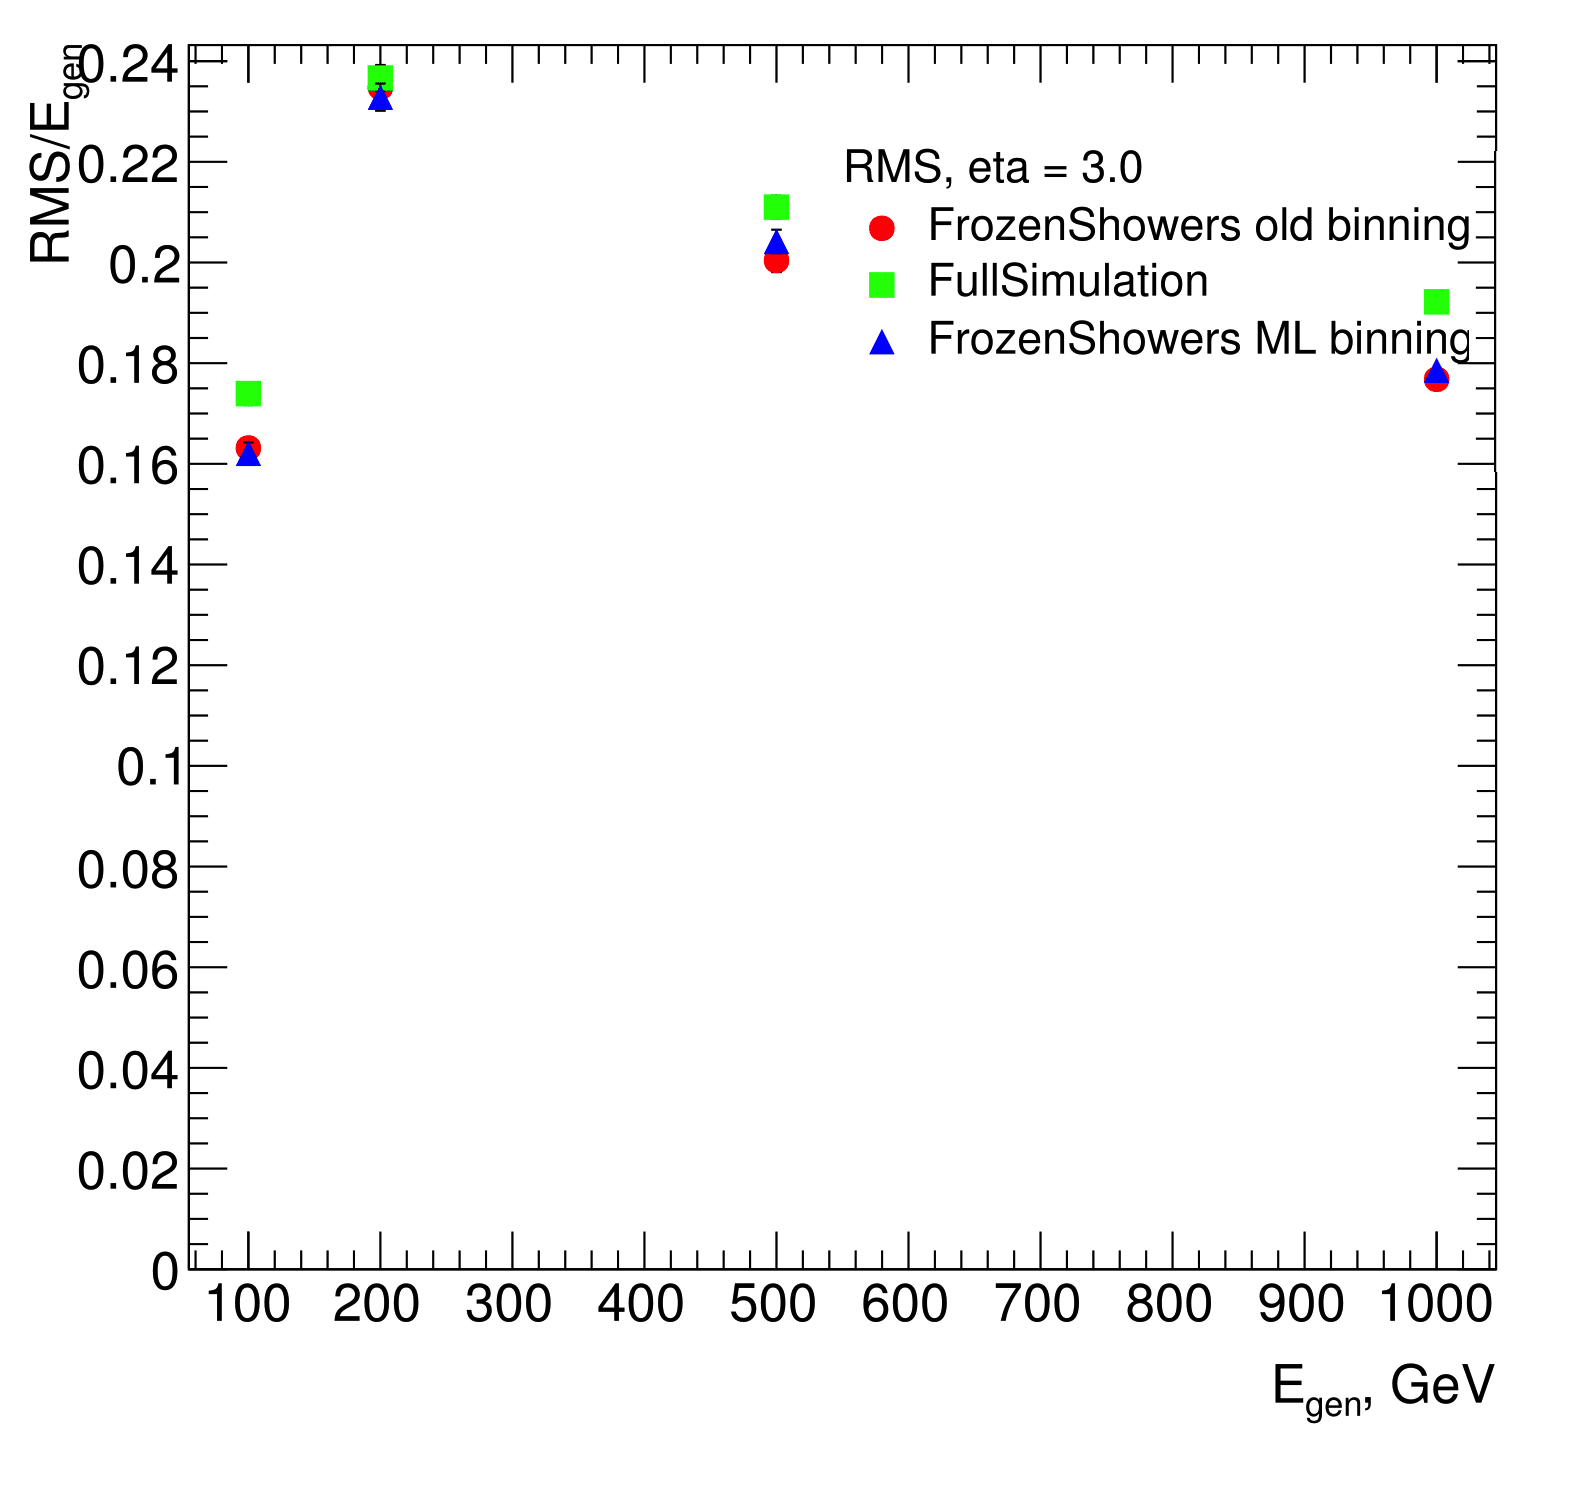
\includegraphics[width=1.\linewidth]{MC/RMS/RMS-12.png} }
\end{minipage}
\hfill
\begin{minipage}[h]{0.45\linewidth}
\center{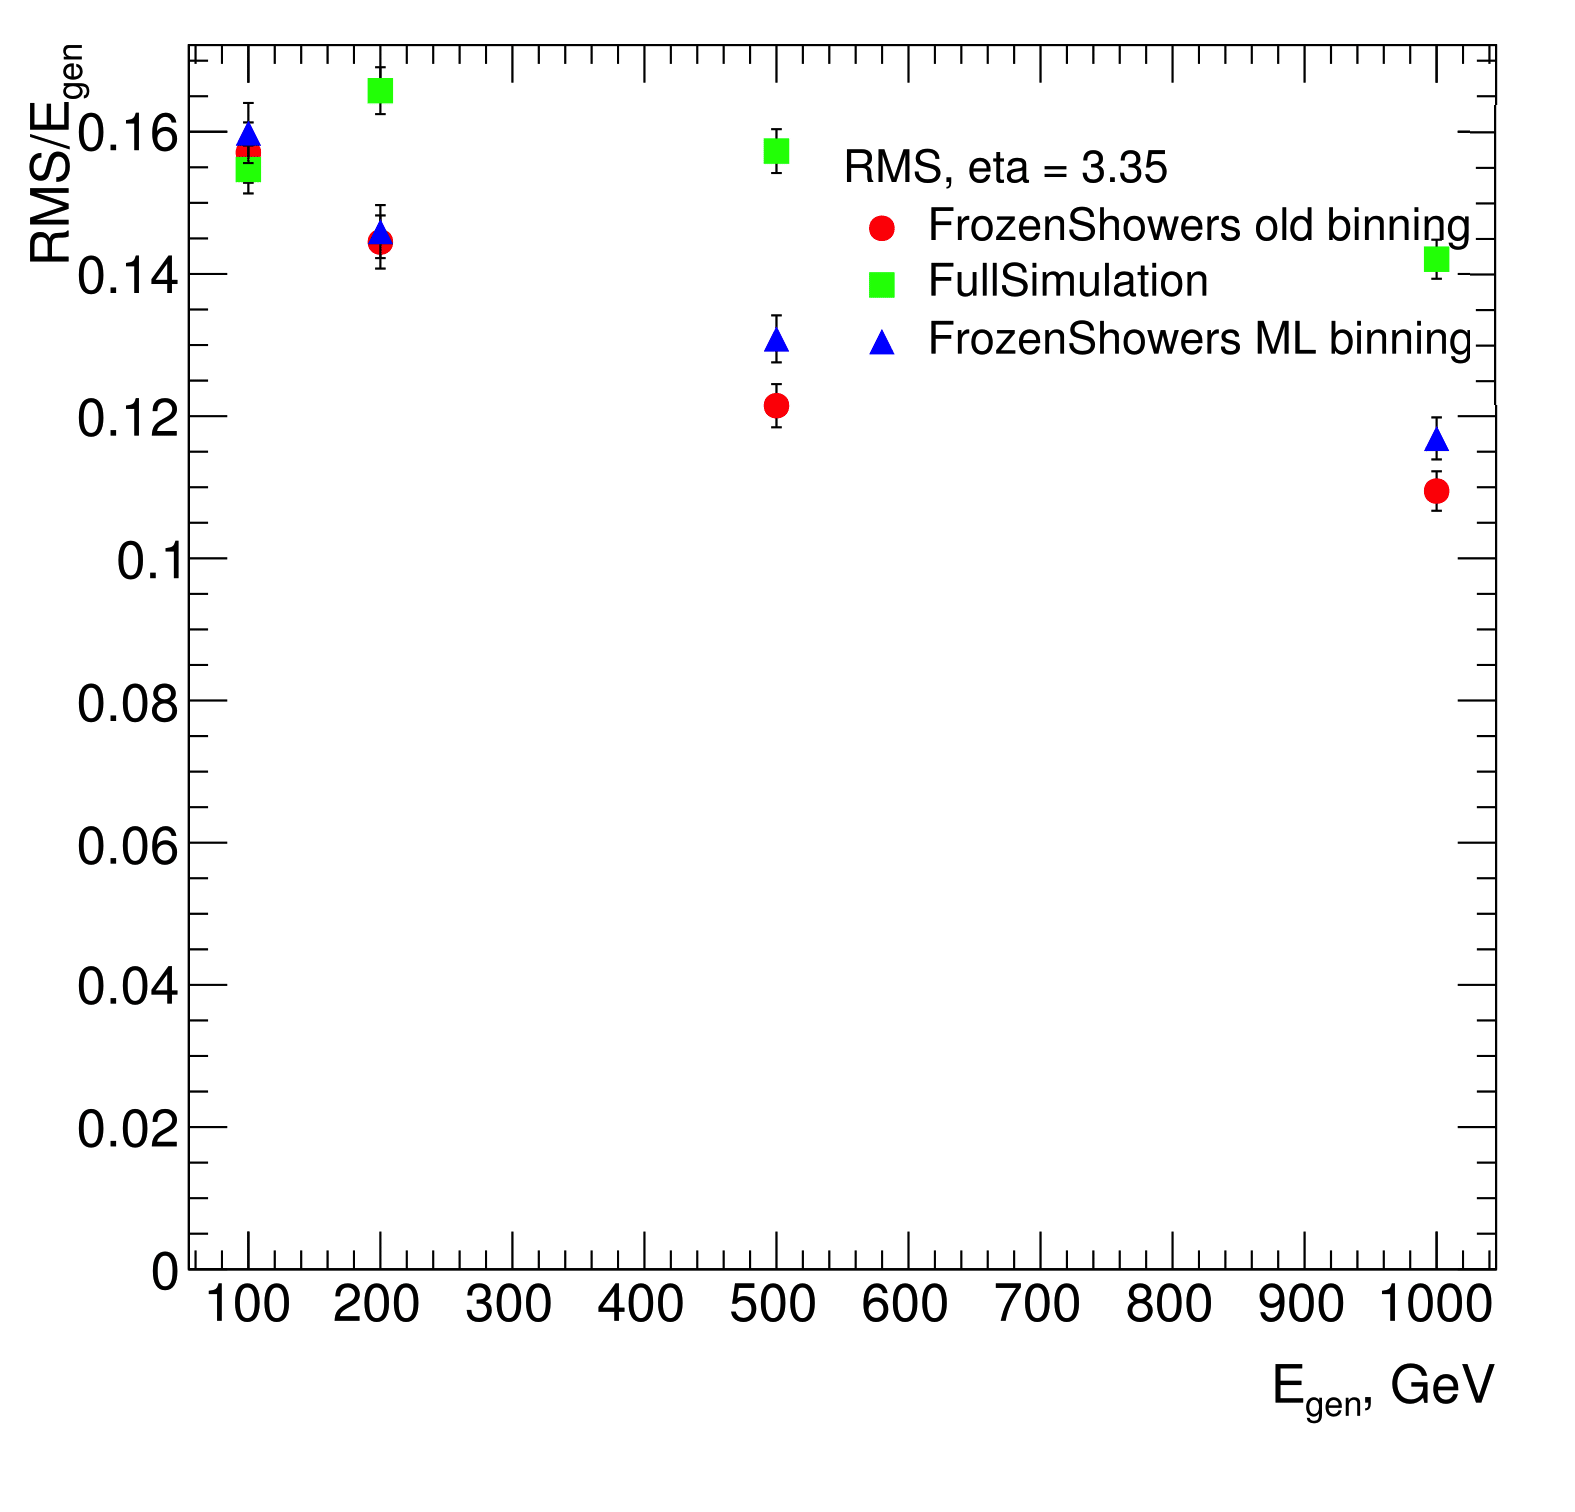
\includegraphics[width=1.\linewidth]{MC/RMS/RMS-11.png} }
\end{minipage}
\vfill
\begin{minipage}[h]{0.45\linewidth}
\center{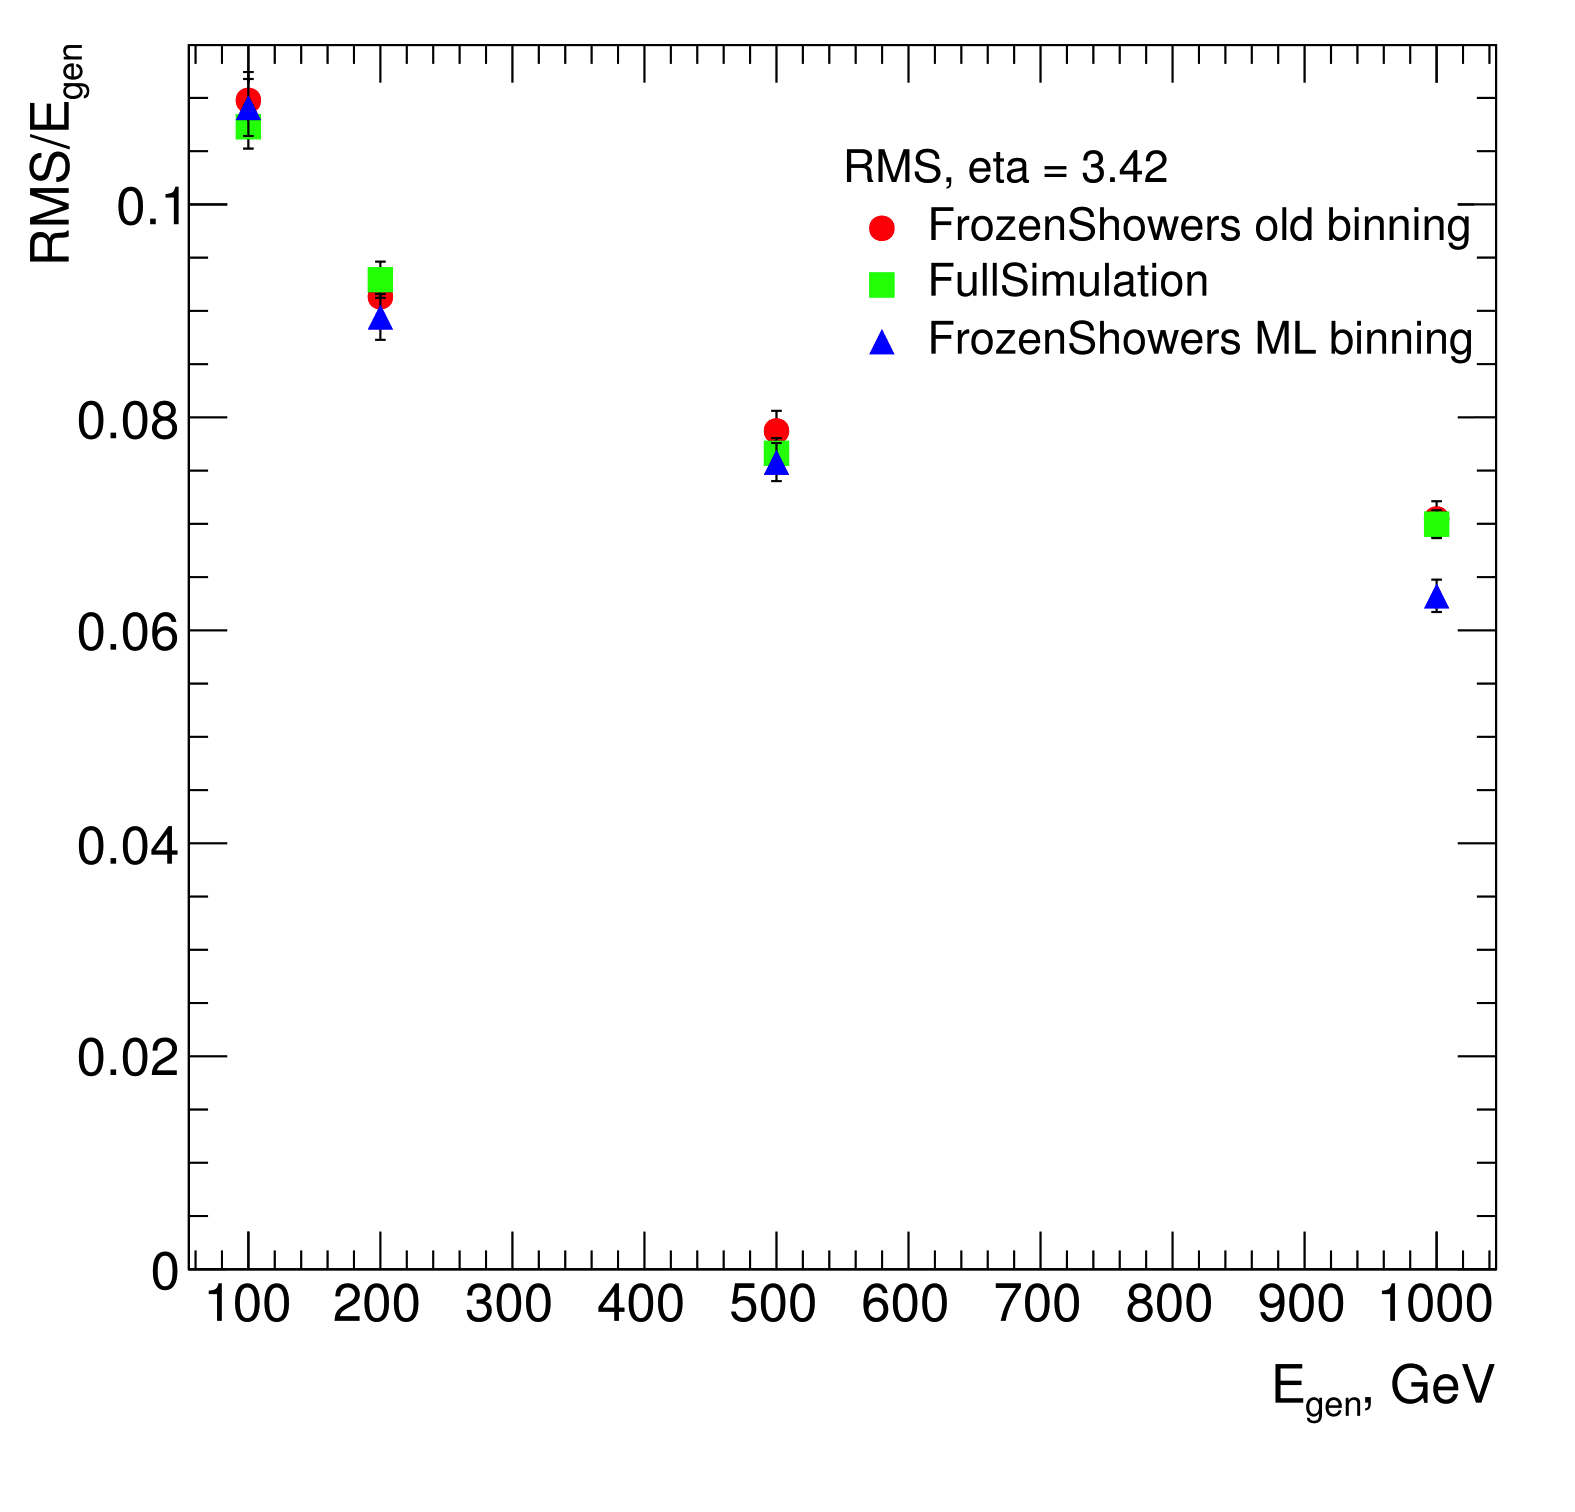
\includegraphics[width=1.\linewidth]{MC/RMS/RMS-10.png}  }
\end{minipage}
\hfill
\begin{minipage}[h]{0.45\linewidth}
\center{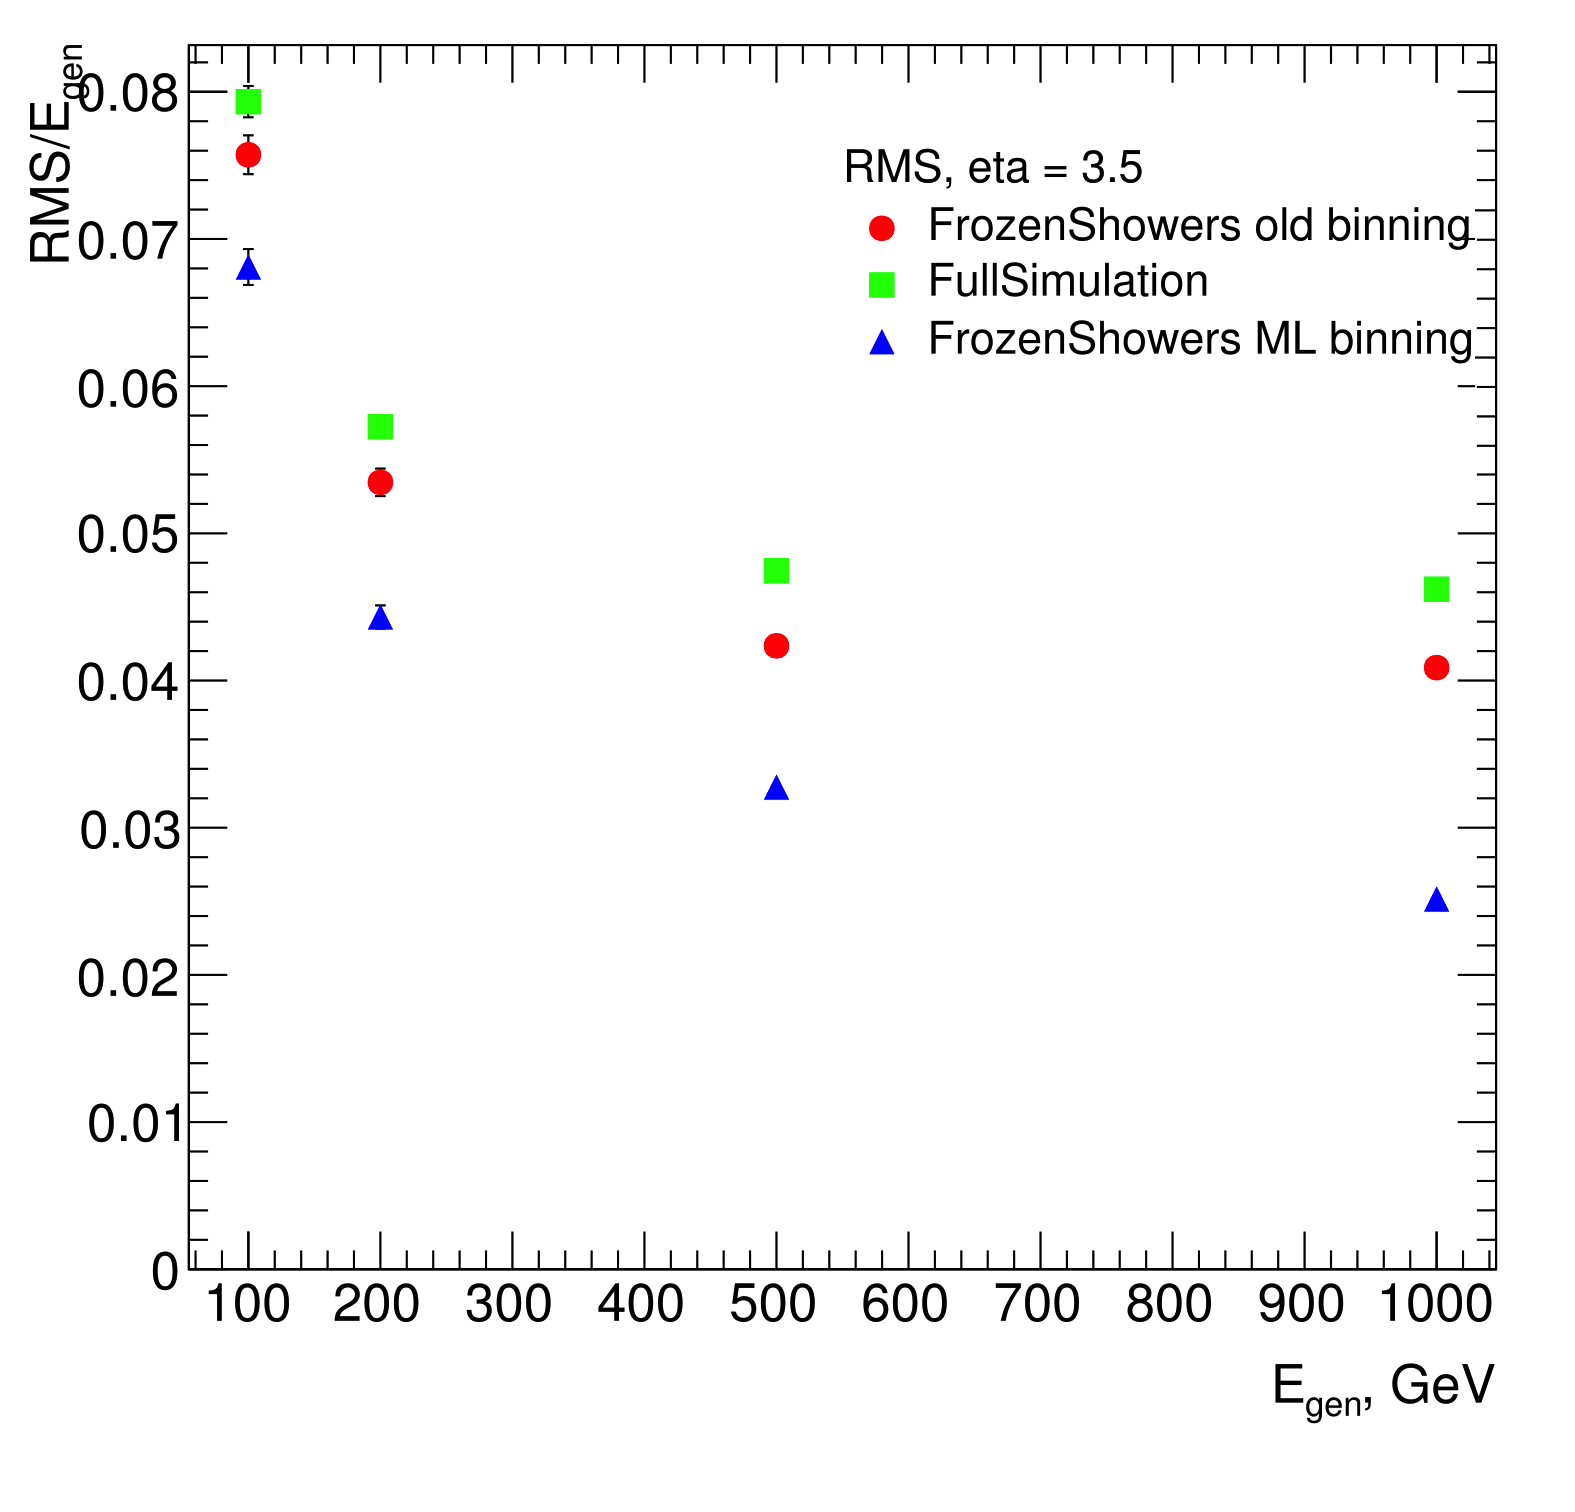
\includegraphics[width=1.\linewidth]{MC/RMS/RMS-09.png}  }
\end{minipage}
\vfill
\begin{minipage}[h]{0.45\linewidth}
\center{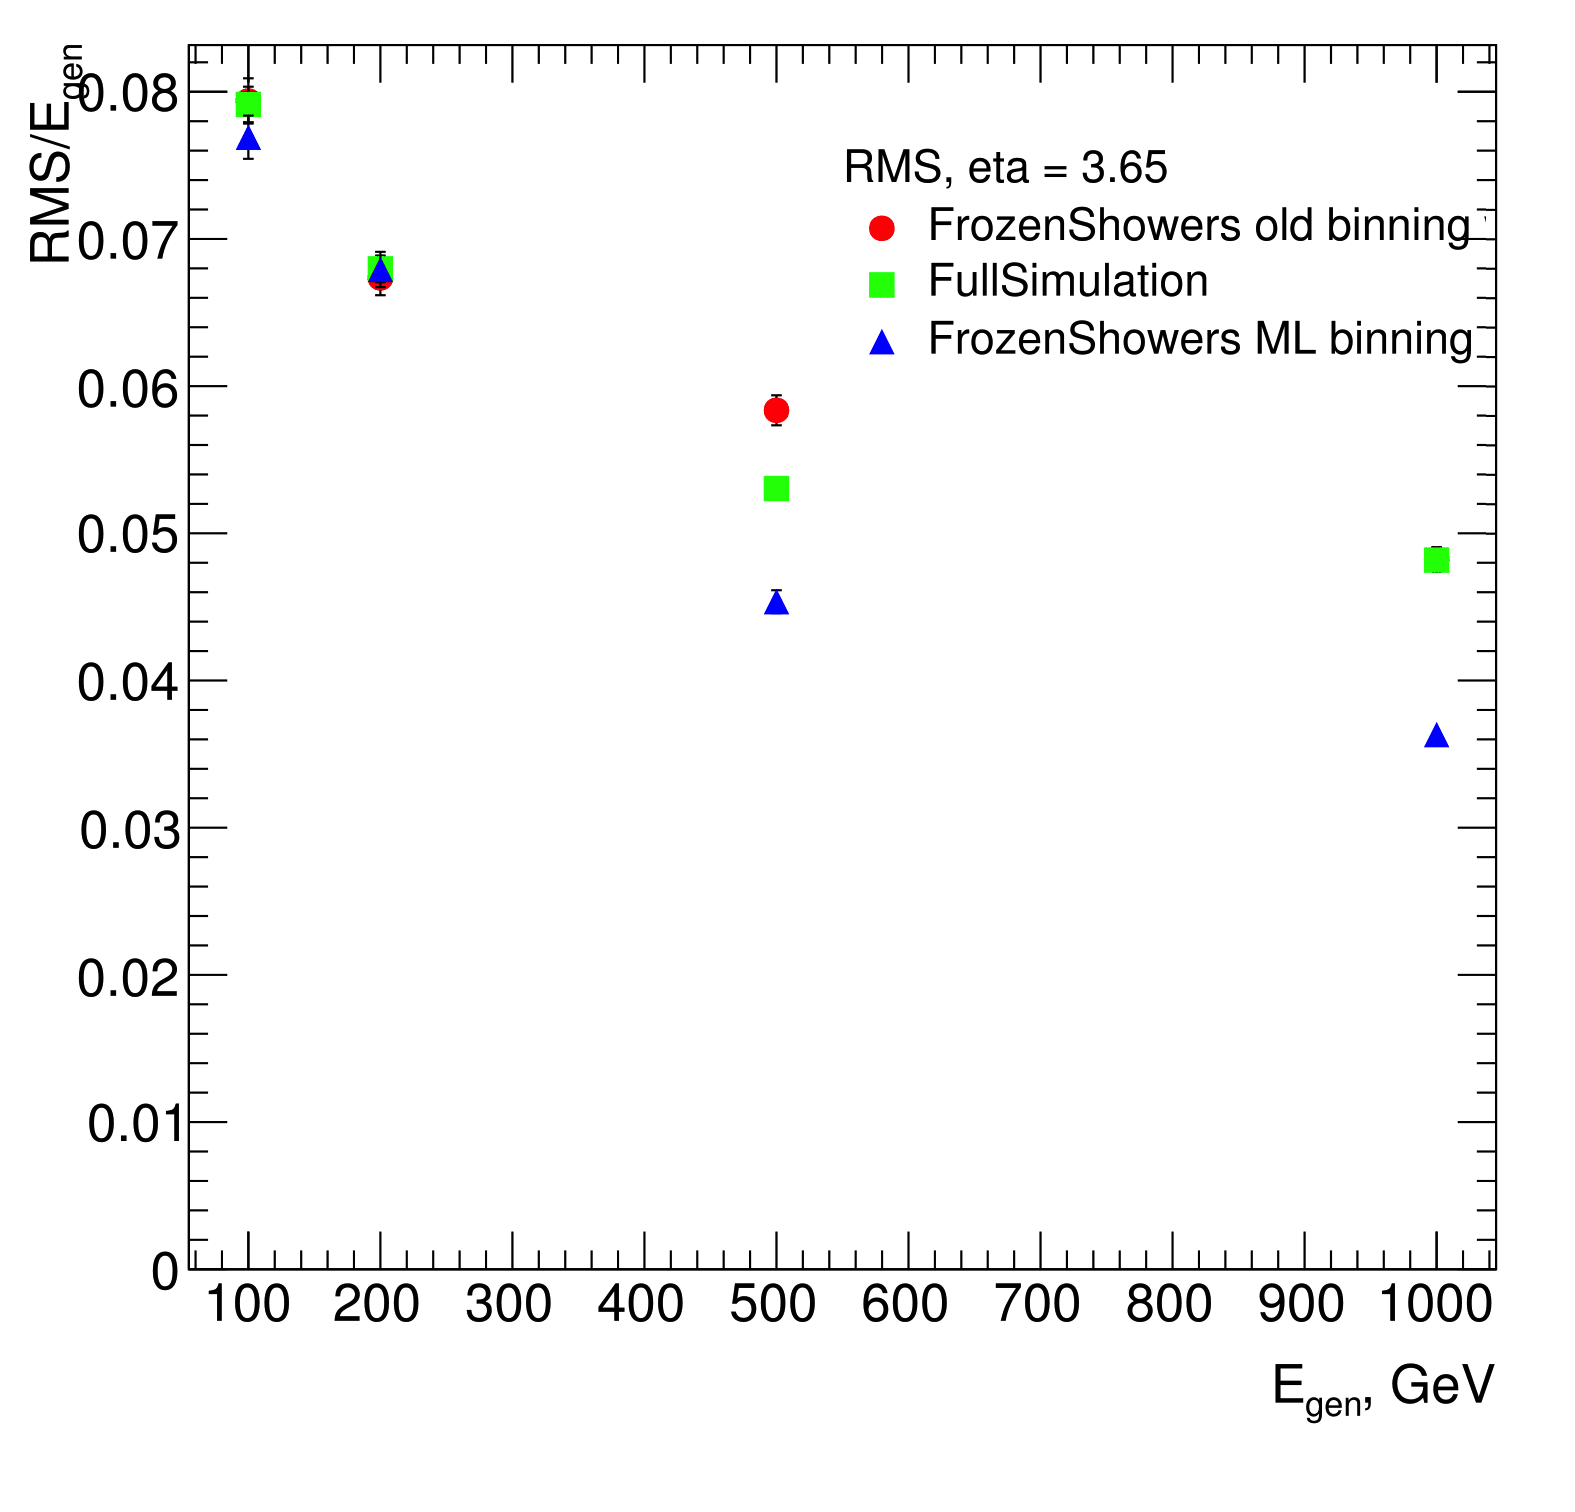
\includegraphics[width=1.\linewidth]{MC/RMS/RMS-08.png} }
\end{minipage}
\hfill
\begin{minipage}[h]{0.45\linewidth}
\center{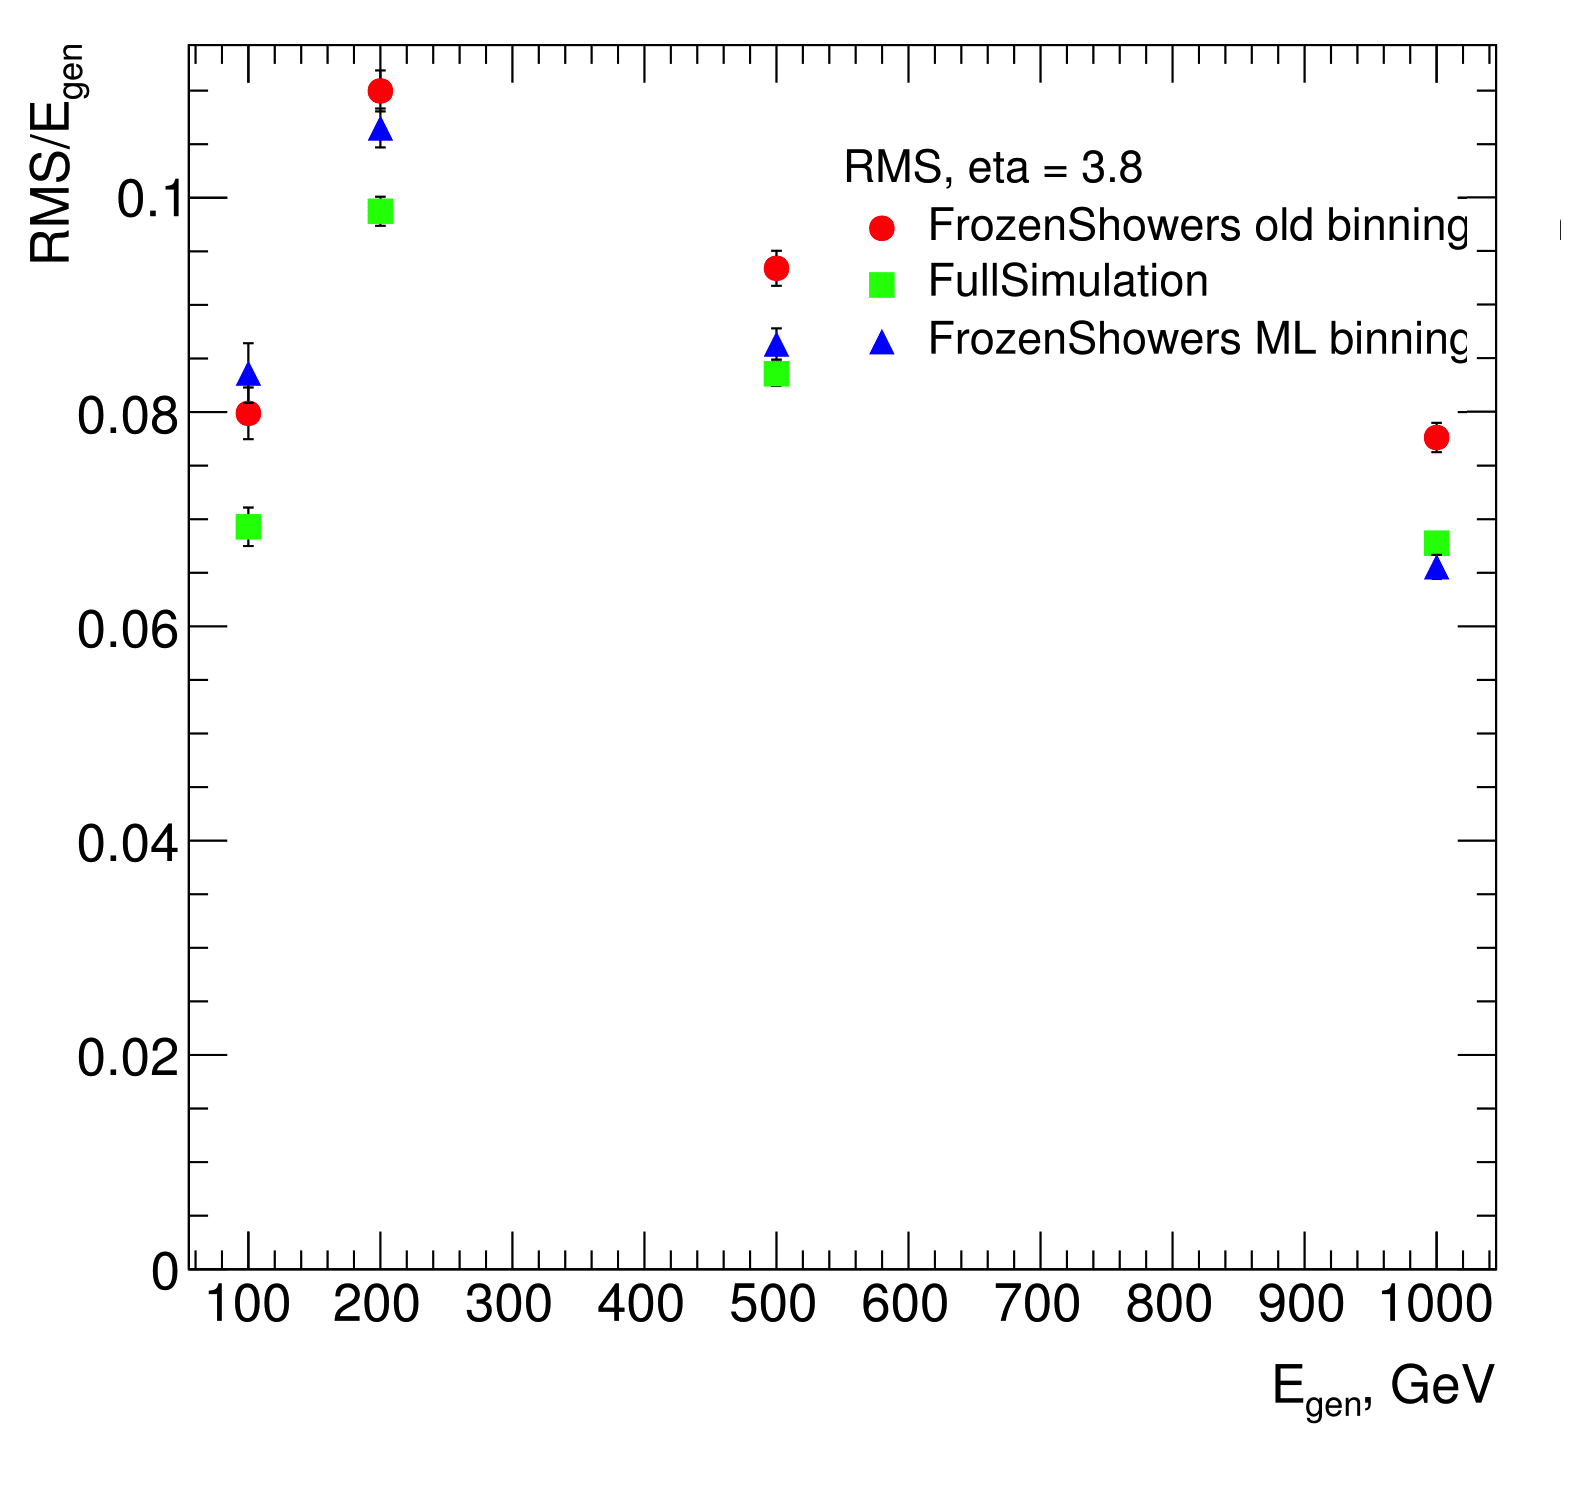
\includegraphics[width=1.\linewidth]{MC/RMS/RMS-07.png}  }
\end{minipage}
\caption{The energy resolution of reconstructed electrons for full simulation, new libraries with machine learning binning and old libraries for different $\eta$ ranges.}
\label{fig:Reso}
\end{figure}

\begin{figure}[!tbp]
\begin{minipage}[h]{0.45\linewidth}
\center{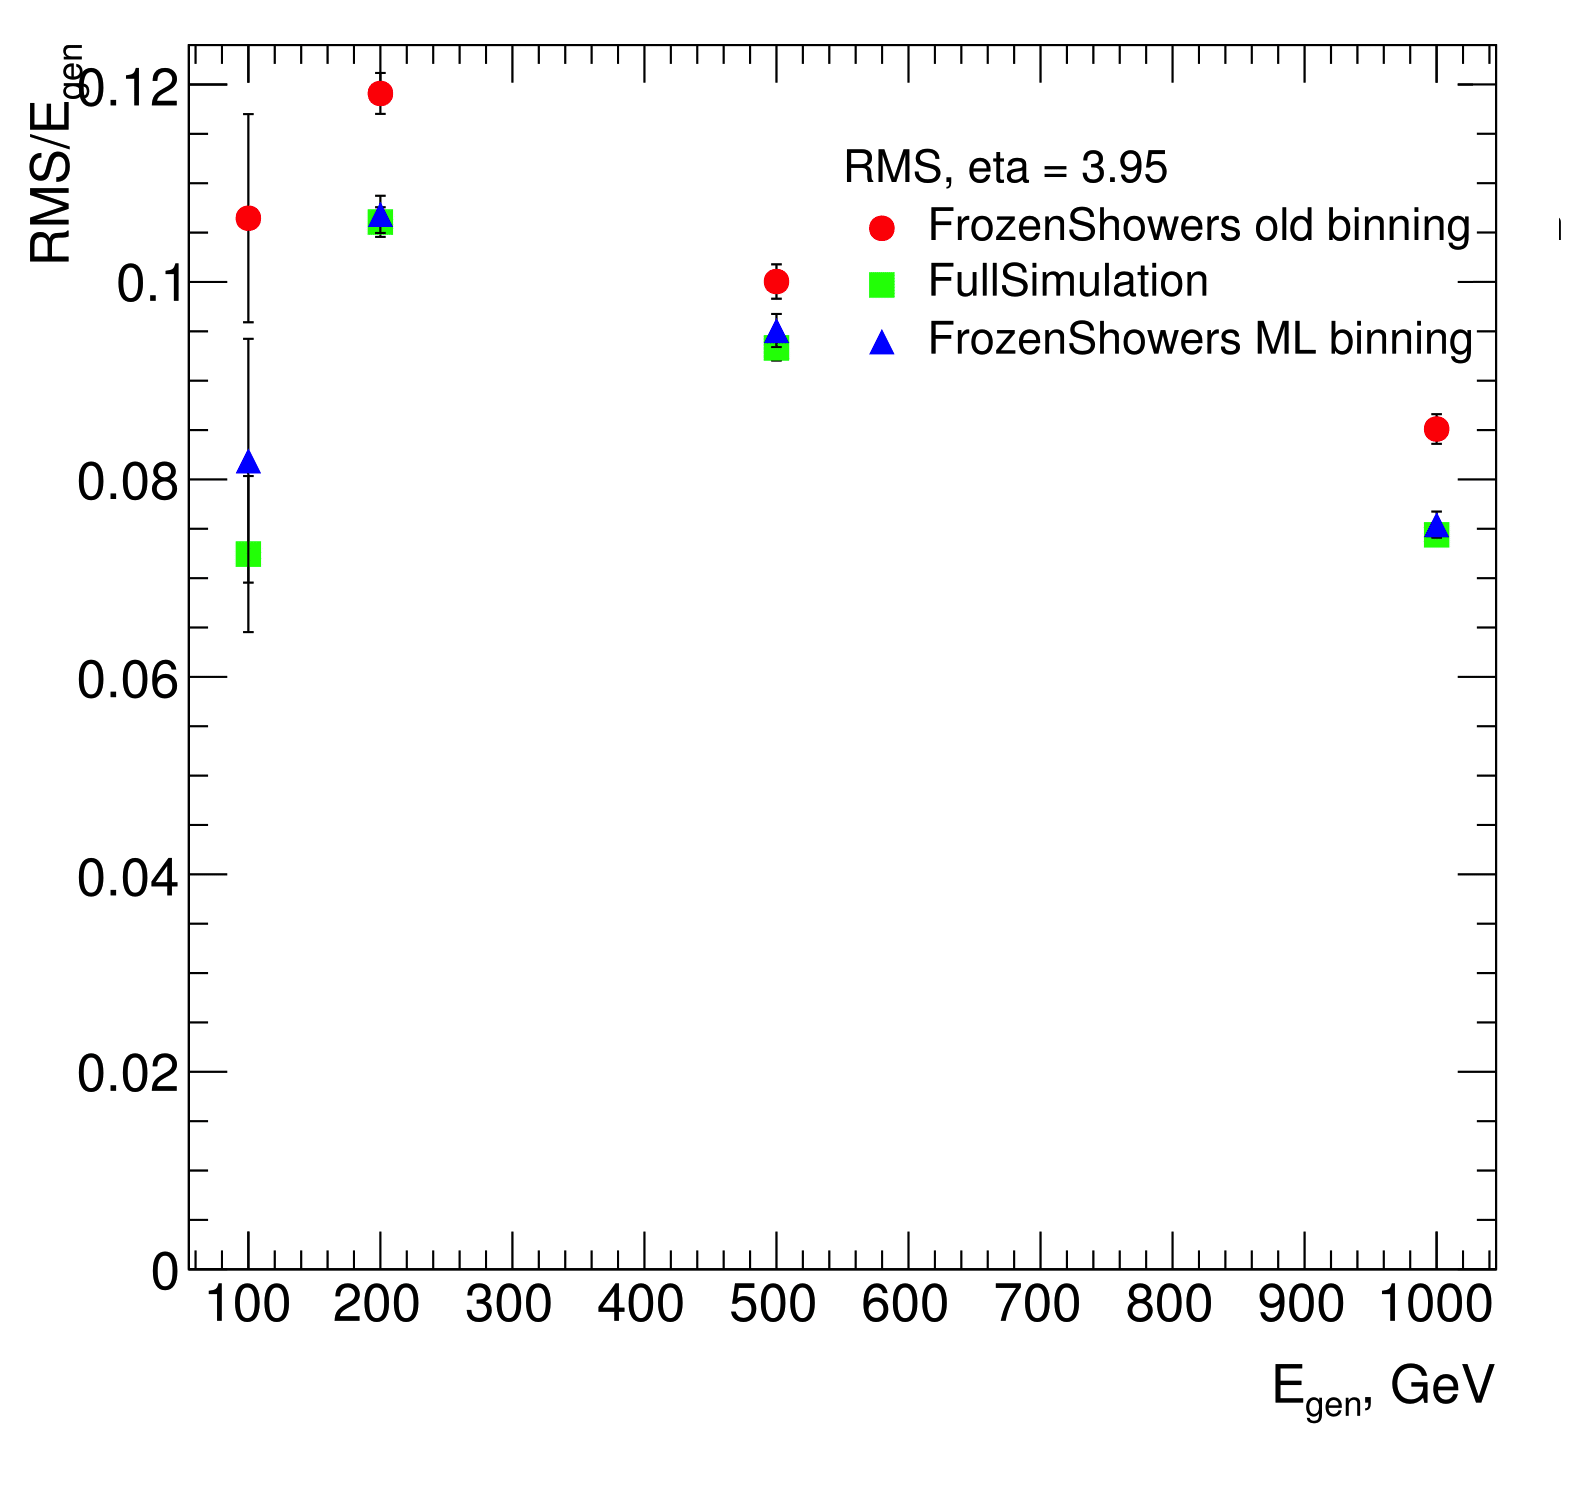
\includegraphics[width=1.\linewidth]{MC/RMS/RMS-06.png}  }
\end{minipage}
\hfill
\begin{minipage}[h]{0.45\linewidth}
\center{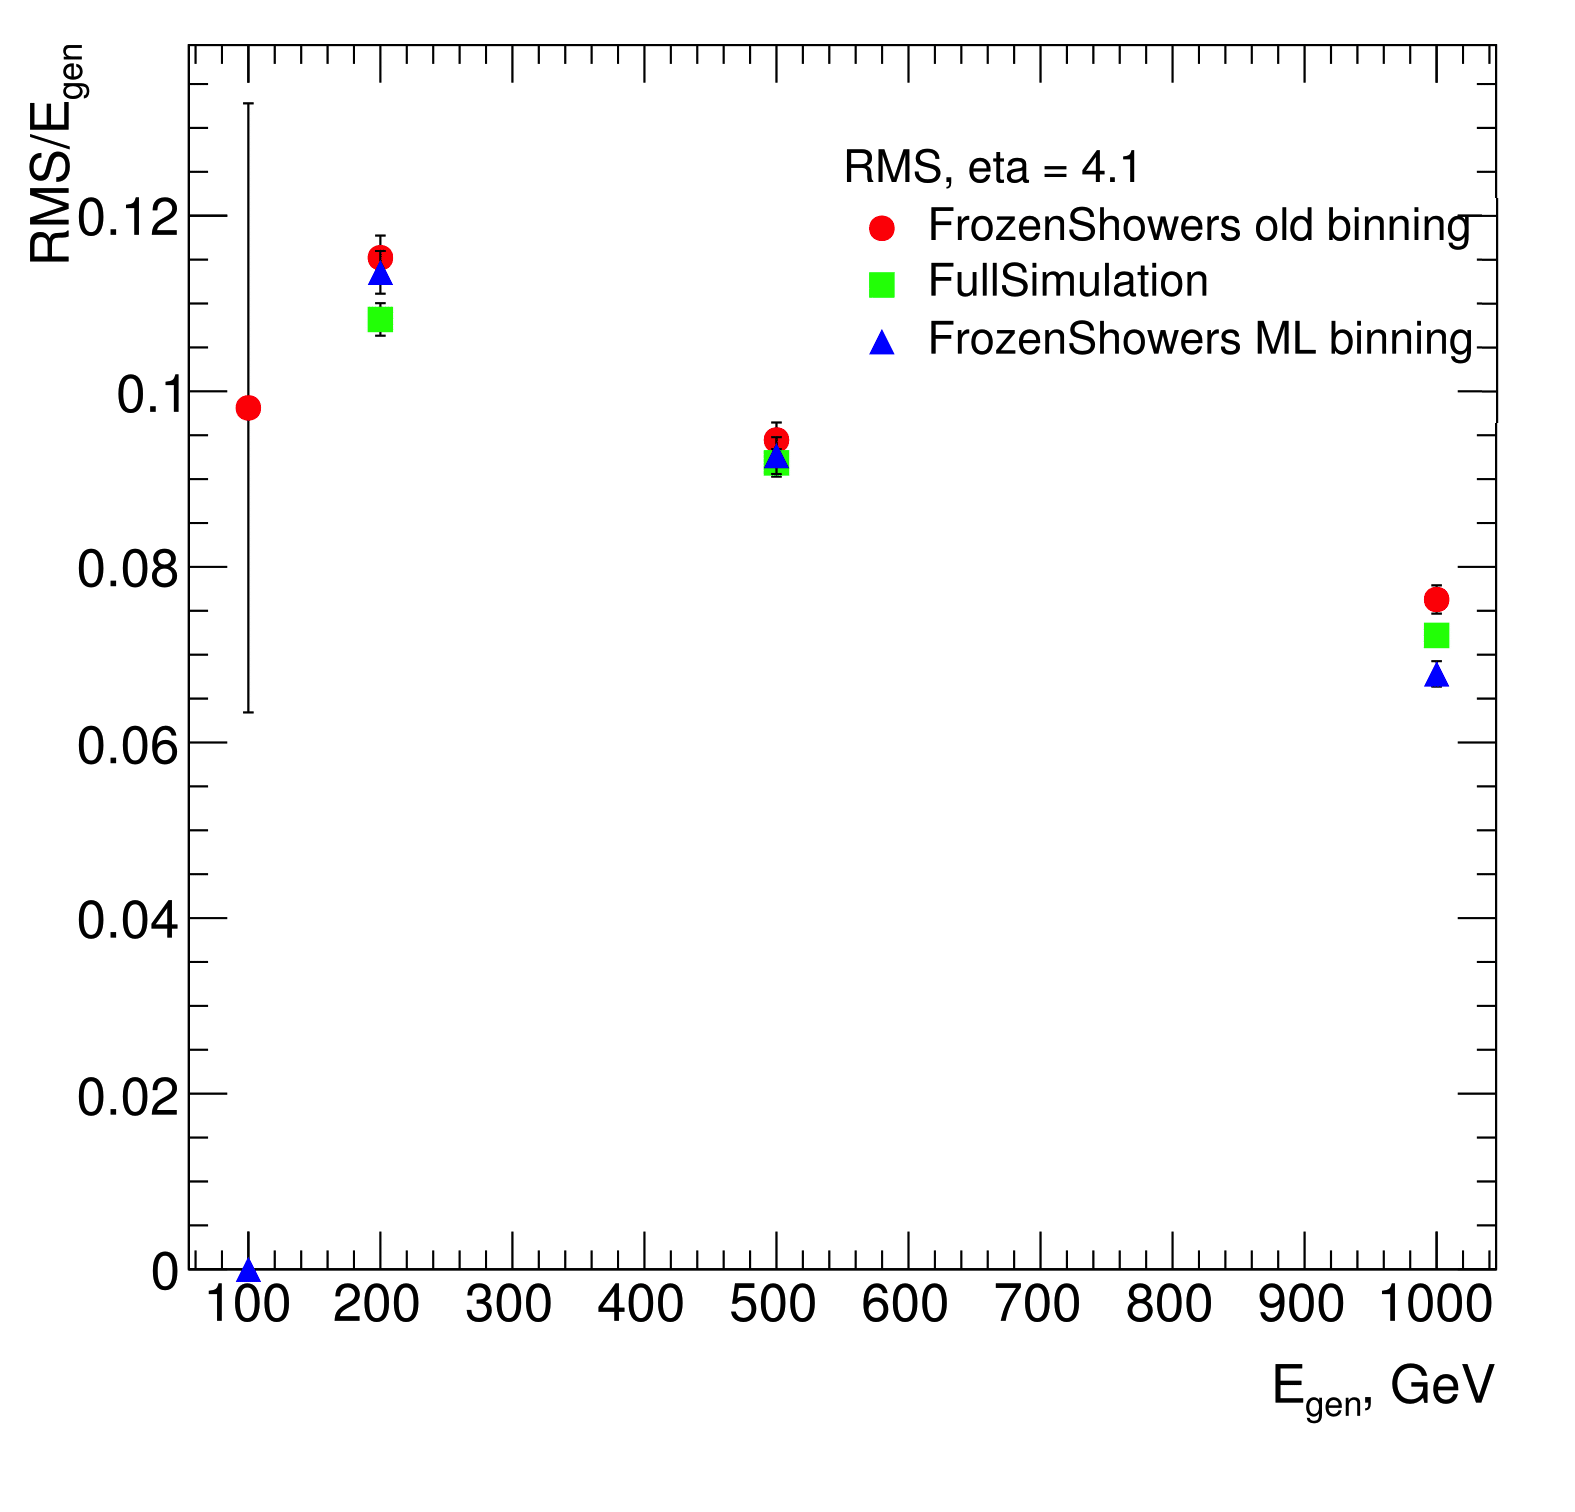
\includegraphics[width=1.\linewidth]{MC/RMS/RMS-05.png}  }
\end{minipage}
\vfill
\begin{minipage}[h]{0.45\linewidth}
\center{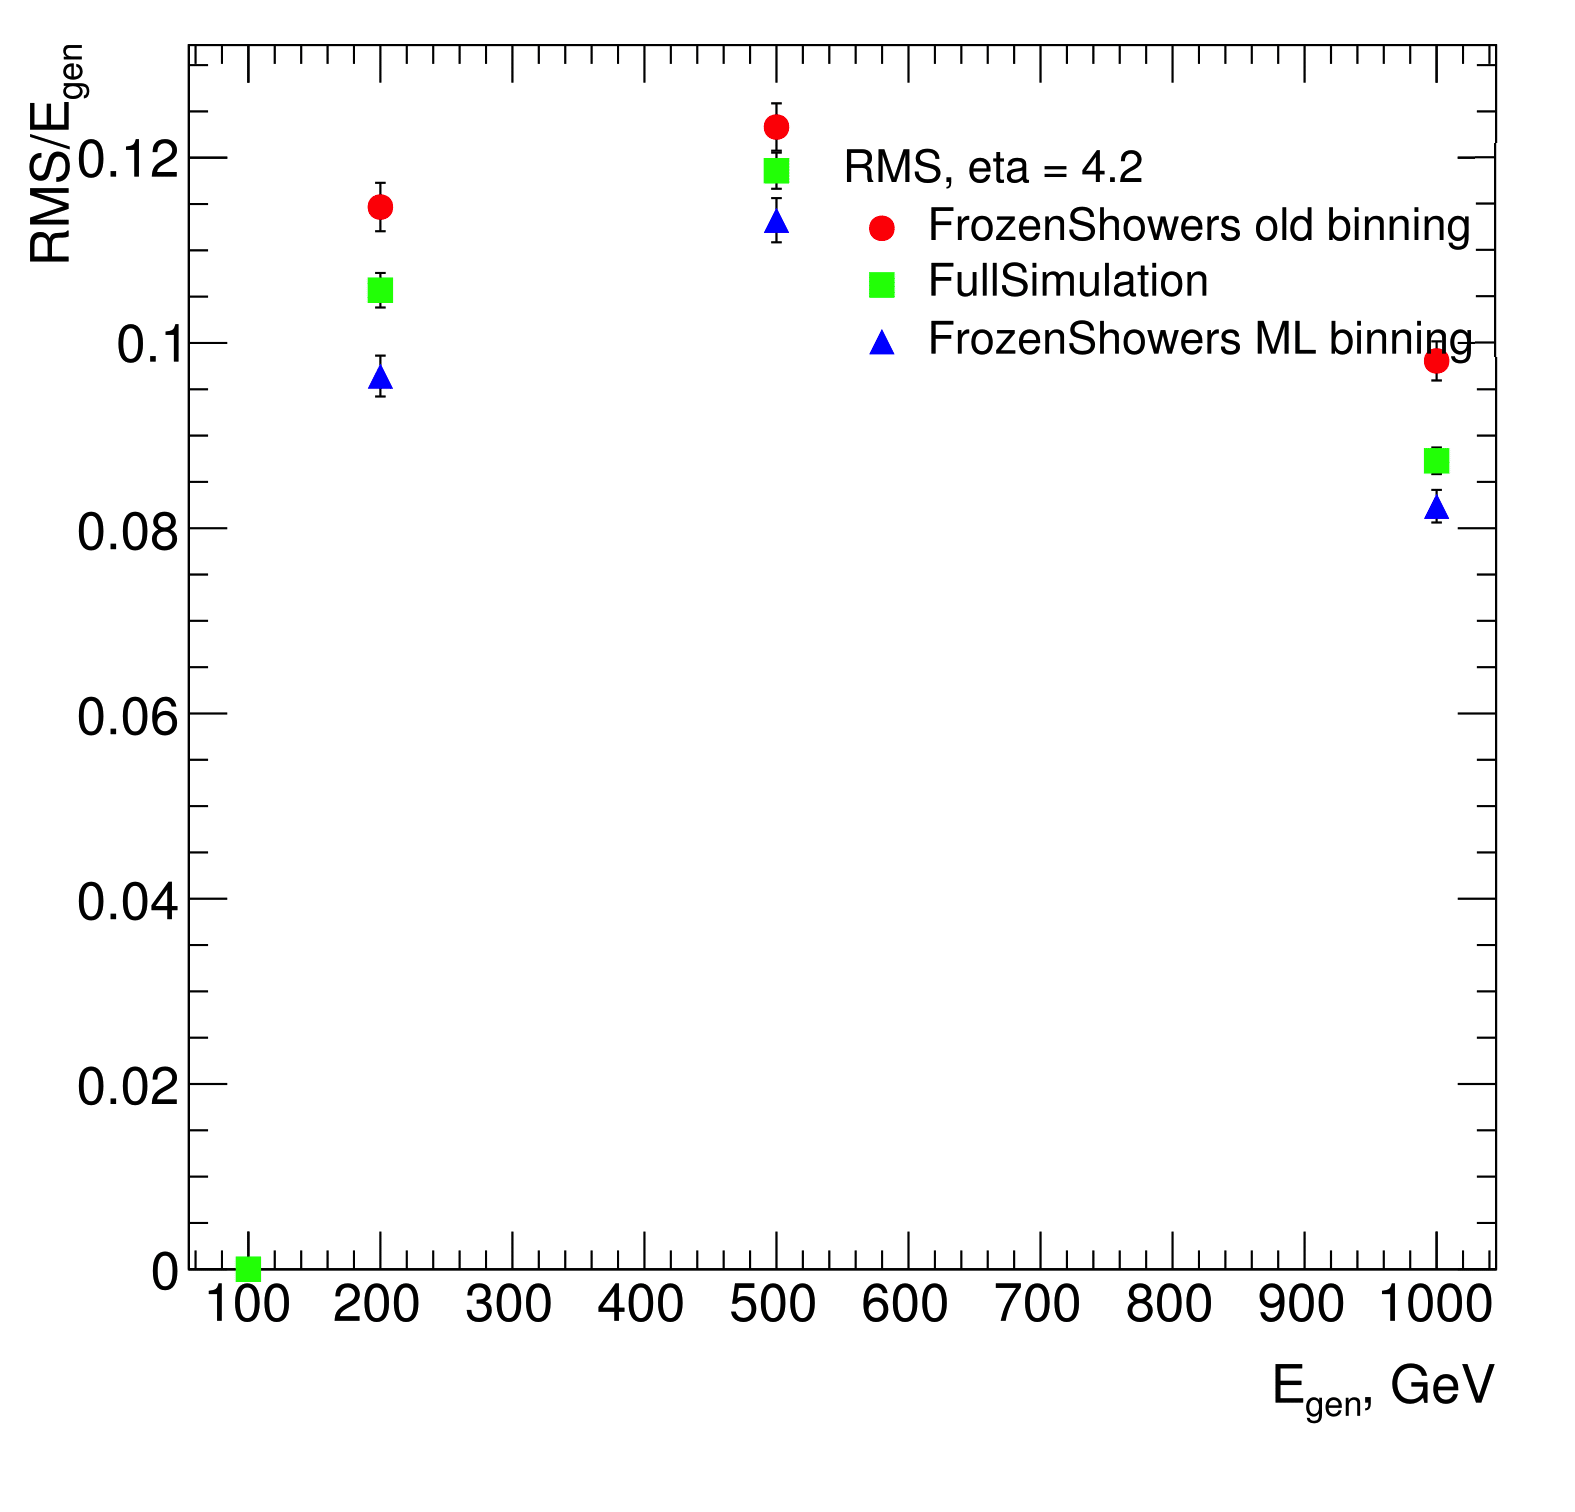
\includegraphics[width=1.\linewidth]{MC/RMS/RMS-04.png}  }
\end{minipage}
\hfill
\begin{minipage}[h]{0.45\linewidth}
\center{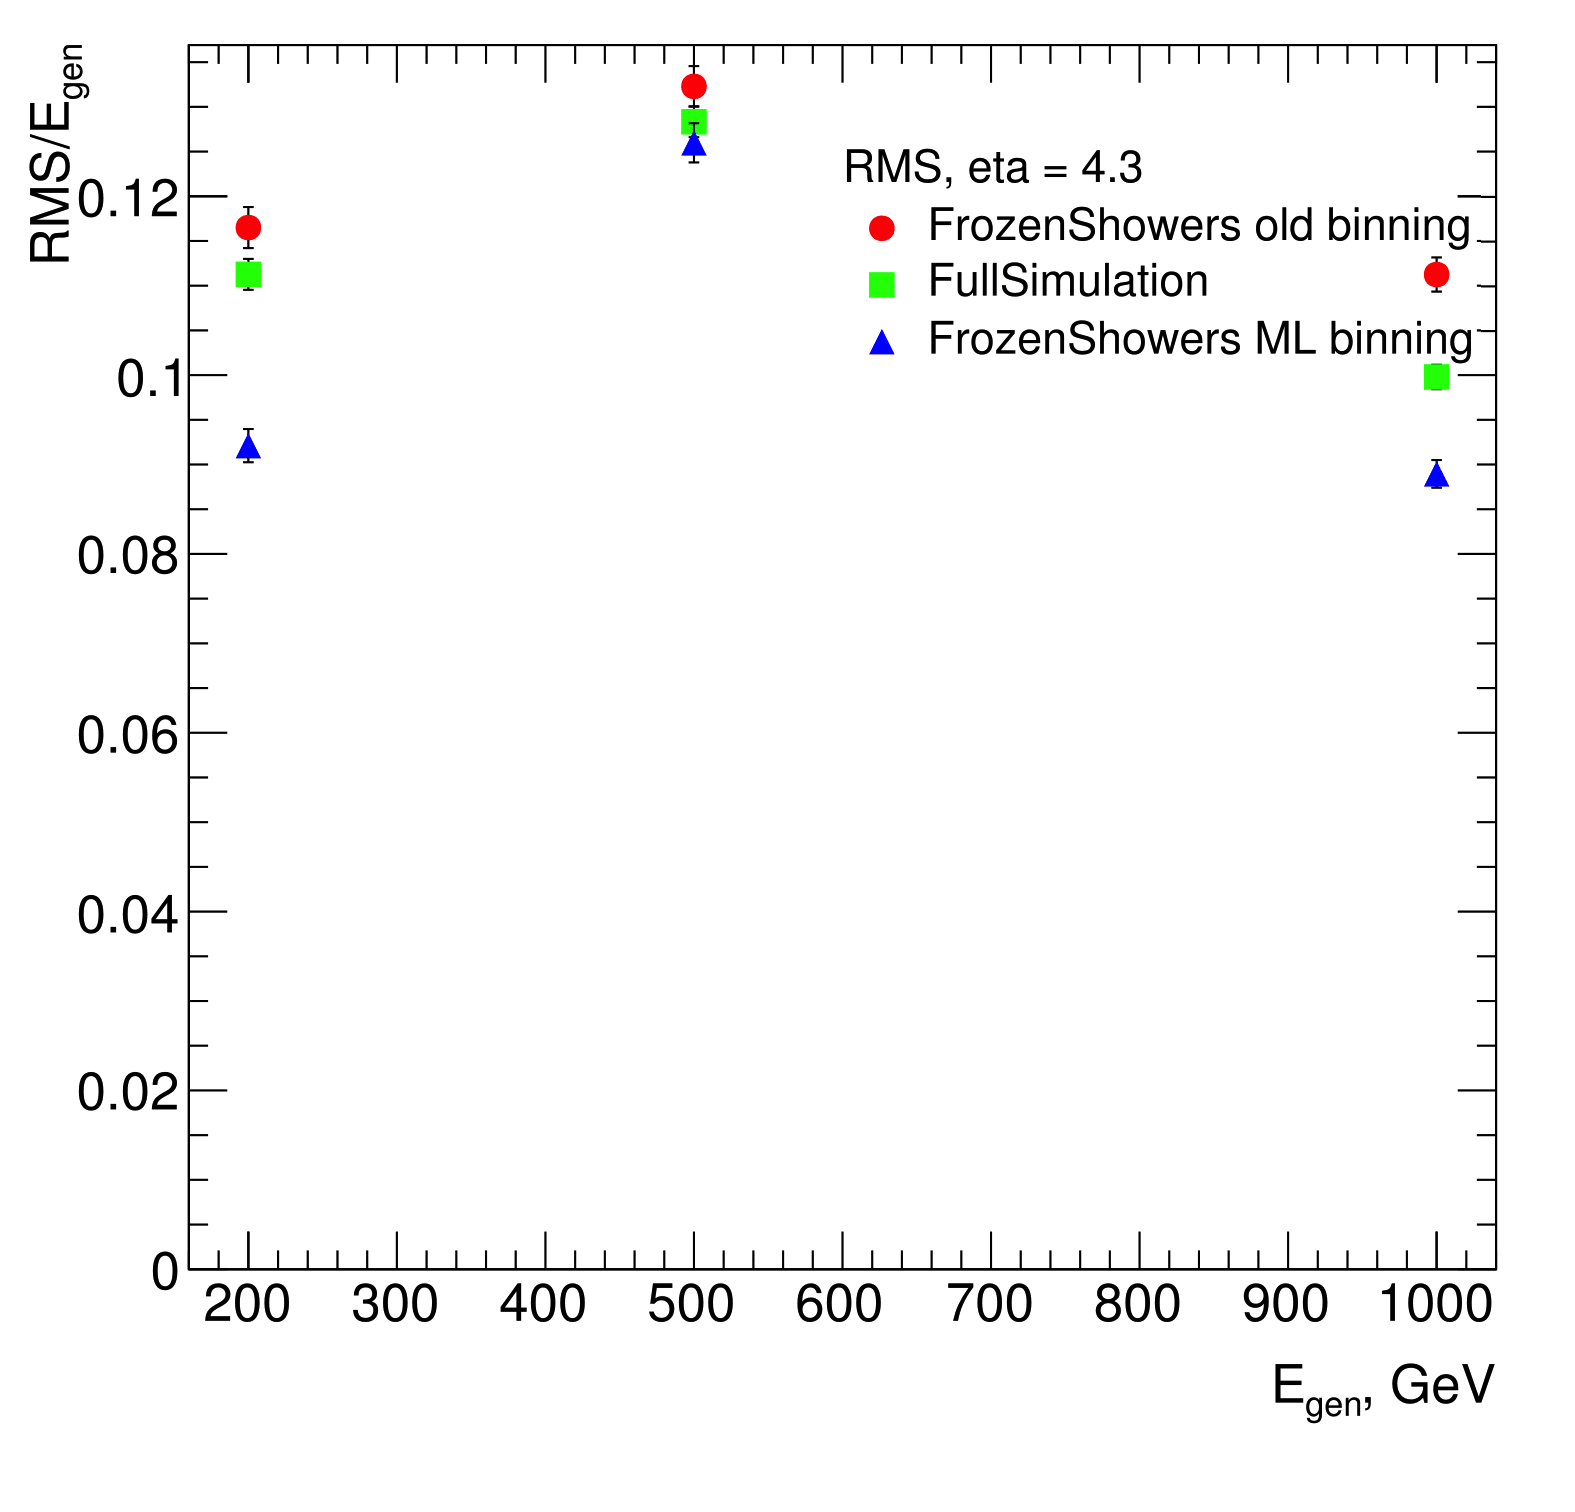
\includegraphics[width=1.\linewidth]{MC/RMS/RMS-03.png}  }
\end{minipage}
\vfill
\begin{minipage}[h]{0.45\linewidth}
\center{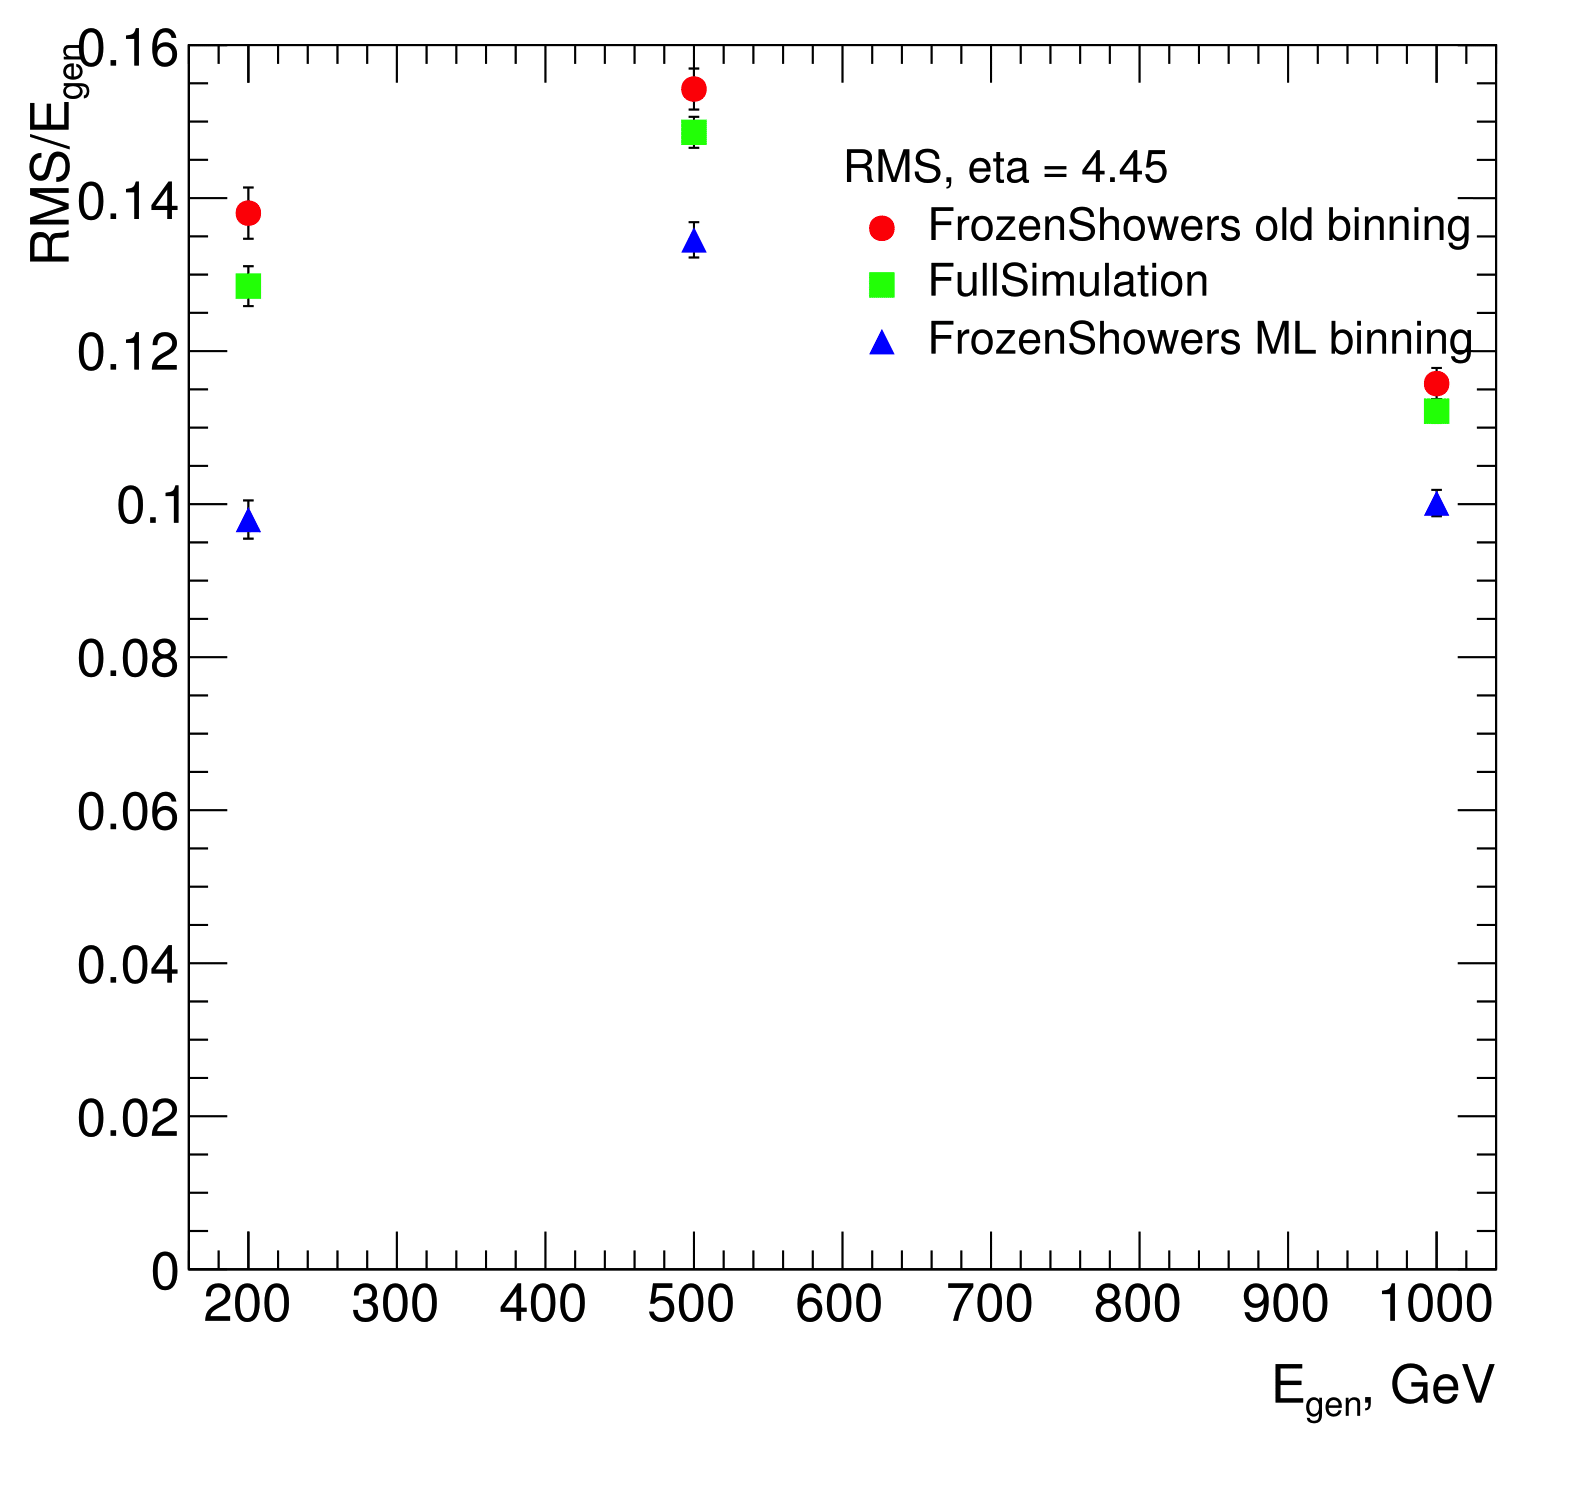
\includegraphics[width=1.\linewidth]{MC/RMS/RMS-02.png} }
\end{minipage}
\hfill
\begin{minipage}[h]{0.45\linewidth}
\center{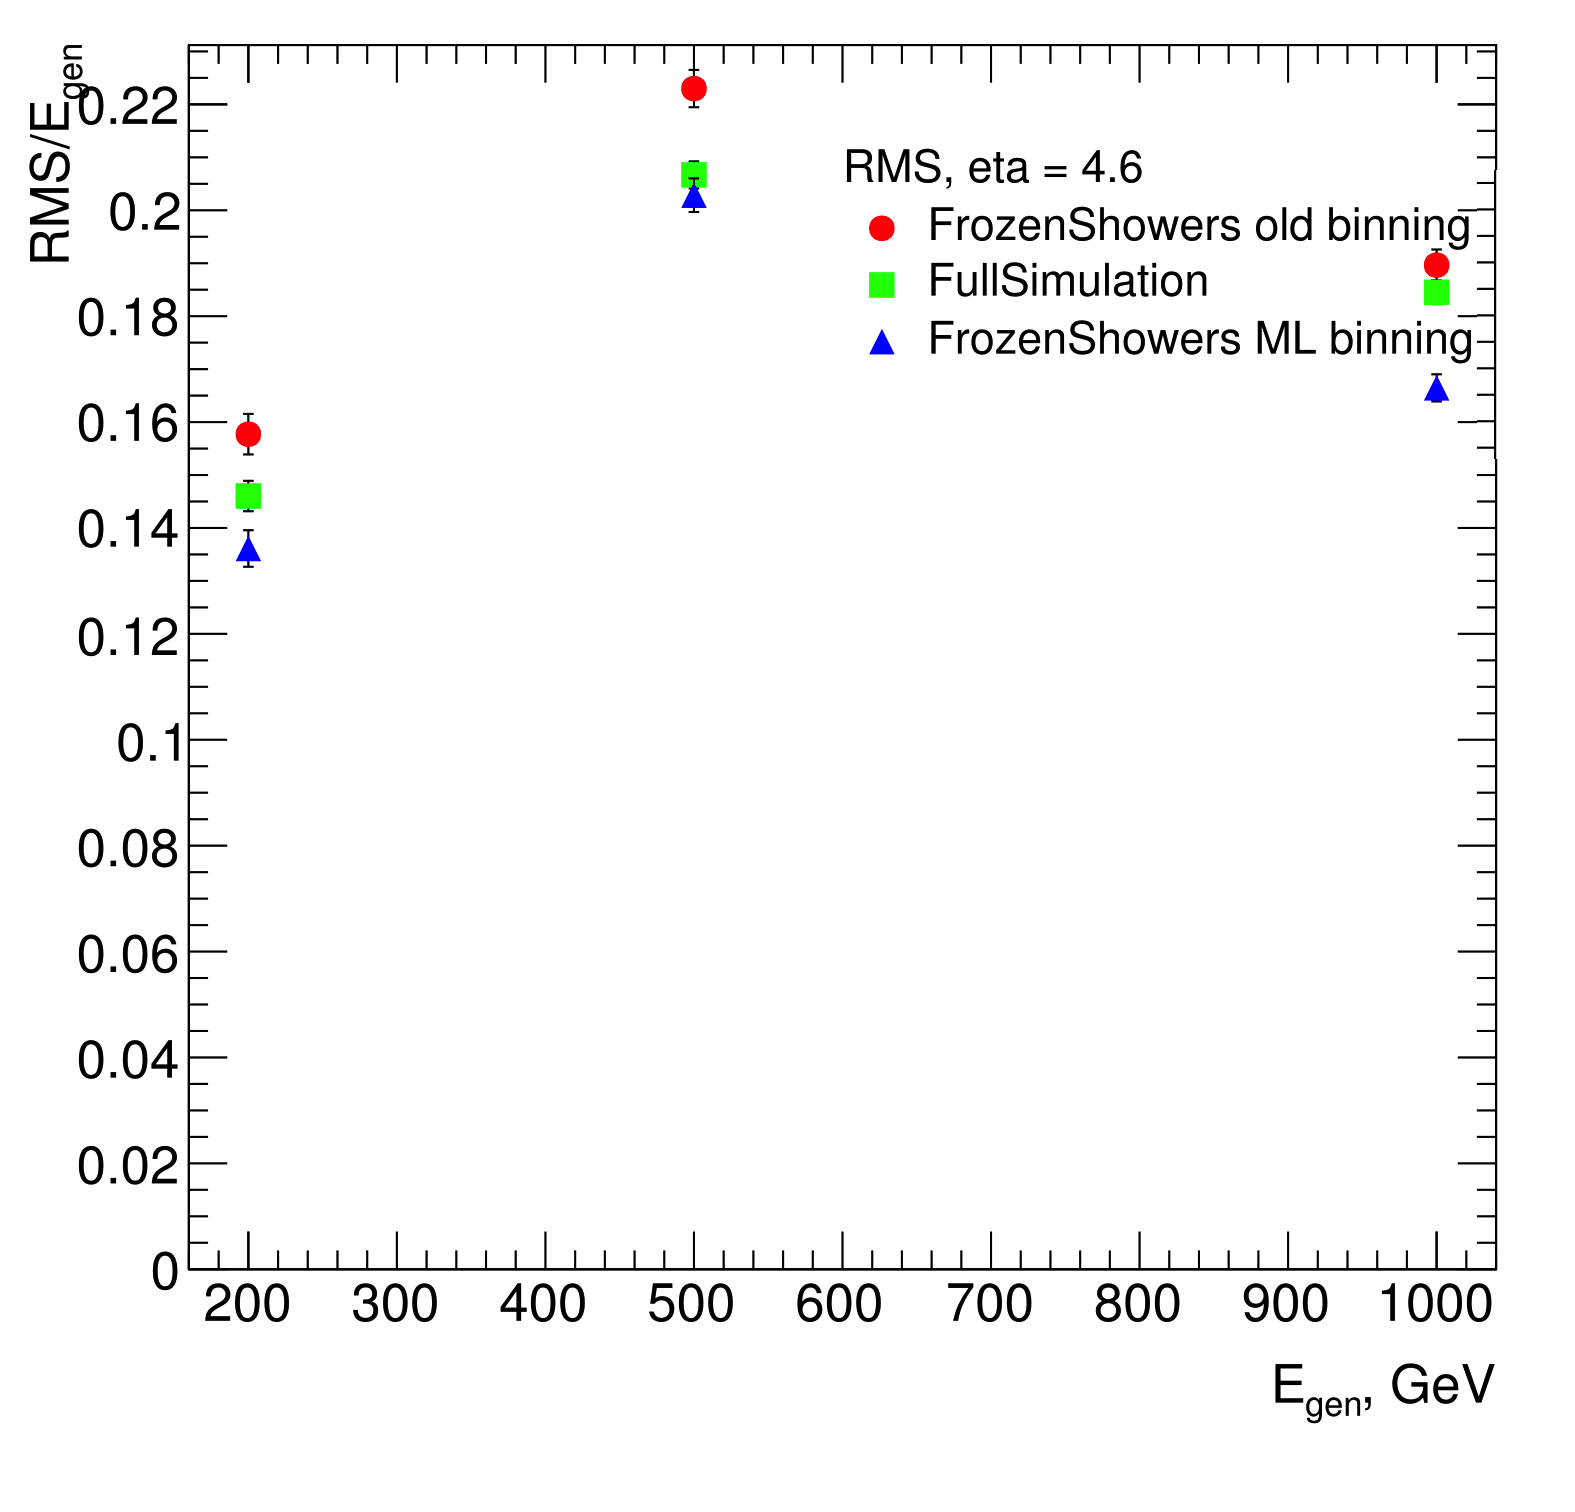
\includegraphics[width=1.\linewidth]{MC/RMS/RMS-01.png} }
\end{minipage}
\caption{The energy resolution of reconstructed electrons for full simulation, new libraries with machine learning binning and old libraries for different $\eta$ ranges.}
\label{fig:Reso2}
\end{figure}

\subsection{Outlook}\label{sec:FSImpr}

The  validation of the electron energy resolution simulation have shown a good agreement between the full and fast simulation  results  for most of the $\eta$-bins, however, this method still can be improved. The following ways of improvement have been investigated and planned to be implemented in the nearest future:
\begin{itemize}
\item $\eta$-dependent bin size. Currently, all of bins have the same width of the liquid argon bin. The procedure should be modified so that the effective width of the liquid argon gap is calculated separately for each $\eta$-bin;
\item Improvement of the training sample. Too simplified training sample could also cause the problem of not perfectly described electron resolution. It is planned  to repeat the training procedure using sample  with the shapes of distributions, closer to the nominal ones;
\item  Addition of a new variable, used in the library (e.g. direction of the shower). Since there is a complex dependency between the position of the electron and its direction (especially in the small energy region), the additional binning could solve the  problems with the electron energy resolution modeling.
\end{itemize}

\section{Validation}\label{sec:FSValidation}

The fast simulation method  should be in a  good agreement with a full simulation results for all  reconstructed objects. The Frozen Showers method is validated using the following physics objects:
\begin{itemize}
\item Z bosons decaying to one central and one forward electrons (Fig.~\ref{fig:OtherVal} a). The mass resolution of Z-boson is dominated by the resolution of the central electron. Therefore is most sensitive to the mean energy of the forward electron. There is a visible shift observed in the mass distribution between the full and fast simulations (Fig.~\ref{fig:OtherValFwd}), however, is within the tolerable region;
\item Jets from two jet events. This validation shows a good agreement with full simulation. The distribution of the jet response (Fig.~\ref{fig:OtherVal} b) show that the Frozen Showers method does not change the jet energy scale;
\item Inclusive forward electron production. The forward electrons validation, that usage of the Frozen Showers is not changing the $\eta$ and $E_{T}$ distributions of the forward electrons.  Studies of the forward electrons resolution have been performed separately and are discussed in the previous section.
\end{itemize}
The total agreement between the full and the fast simulation results for different observables justifies the usage of the  Frozen Showers method in an official ATLAS MC simulation production.

\begin{figure}[!tbp]
\begin{minipage}[h]{0.49\linewidth}
\center{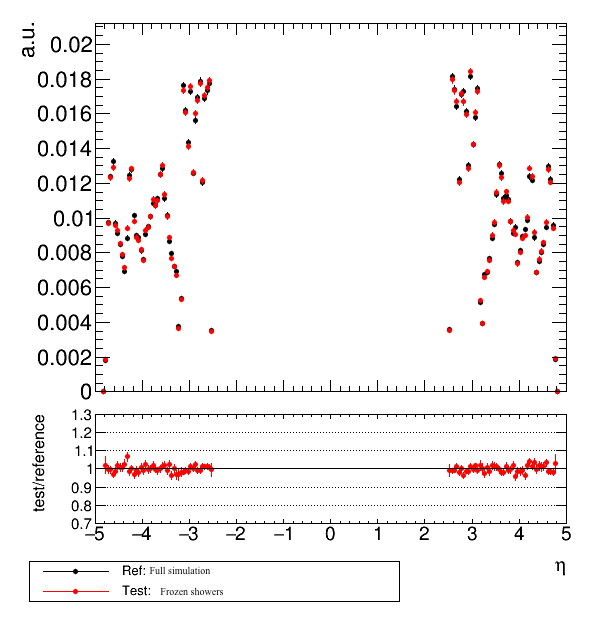
\includegraphics[width=1.\linewidth]{MC/Electron_Frwd_All_KinPlots_eta.png} \\ a)}
\end{minipage}
\hfill
\begin{minipage}[h]{0.49\linewidth}
\center{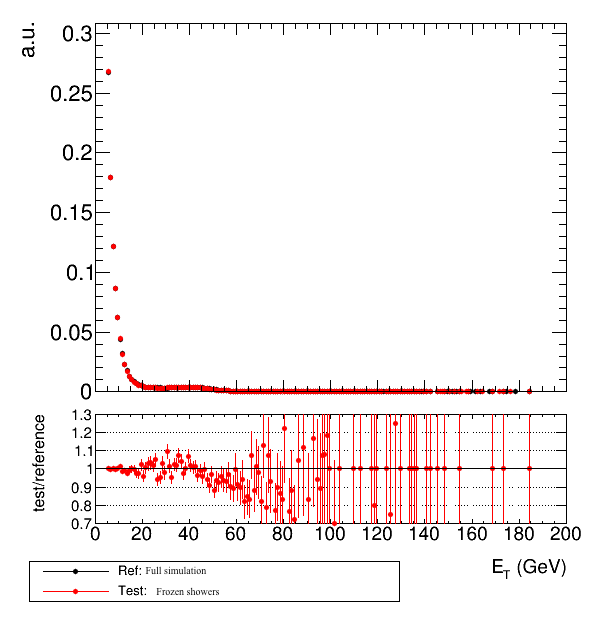
\includegraphics[width=1.\linewidth]{MC/Electron_Frwd_All_KinPlots_et.png} \\ b)}
\end{minipage}
\caption{Results of validation of the Frozen Showers library on forward electrons. Comparison between full simulation and fast simulation using Frozen Showers in forward electron events  a) electron pseudorapidity and b) electron transverse energy. Modified from \cite{ElecForwardVal}. }
\label{fig:OtherValFwd}
\end{figure}

\begin{figure}[!tbp]
\begin{minipage}[h]{0.49\linewidth}
\center{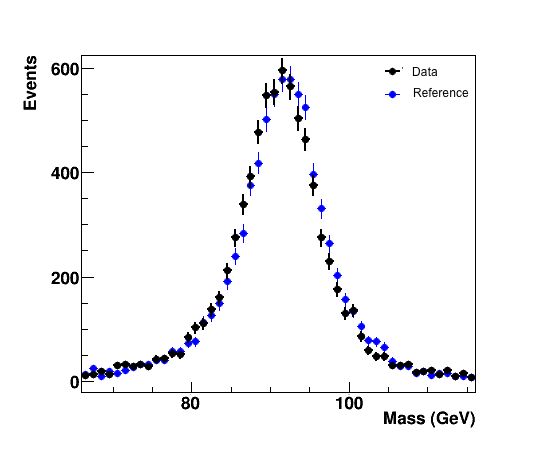
\includegraphics[width=1.\linewidth]{MC/Zee_FWDZee_ZMassFWDTight.png} \\ a)}
\end{minipage}
\hfill
\begin{minipage}[h]{0.49\linewidth}
\center{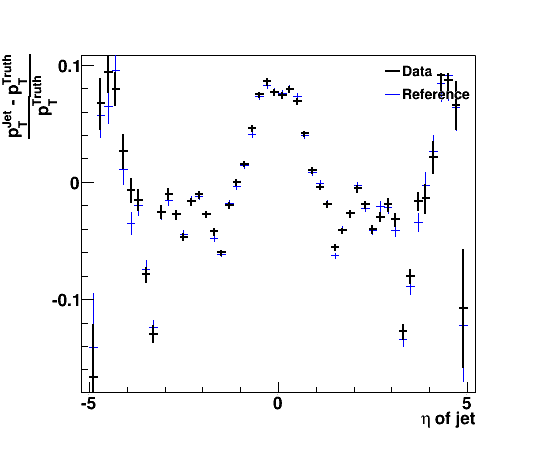
\includegraphics[width=1.\linewidth]{MC/erhResponseVsEta.png} \\ b)}
\end{minipage}
\caption{ Results of validation of the Frozen Showers library on $Z \to ee$ and jets sample. Comparison between full simulation and fast simulation using Frozen Showers for and a) mass of the dilepton pair in $Z \to ee$ candidate events (modified from \cite{ZeeVal}) b) jets response vs  pseudorapidity  distribution (modified from \cite{JetsVal}). }
\label{fig:OtherVal}
\end{figure}
